\documentclass[11pt,letterpaper]{amsart}
\usepackage[
    paperwidth=8.5in,
    paperheight=11in,
    margin=1.25in,
    marginparwidth=0.75in,
    marginparsep=0.1in,
    footskip=0.25in
]{geometry}

\renewcommand{\baselinestretch}{1.}
\setlength{\parindent}{2em}
\setlength{\parskip}{2pt}
\usepackage[shortlabels]{enumitem}
\setlist{
    itemsep=1ex,
    listparindent=\parindent,
    parsep=0em,
    topsep=2ex,
}
\setcounter{tocdepth}{1}
\allowdisplaybreaks[1]

\usepackage{xpatch}
\usepackage{amsfonts}
\usepackage{amsmath}
\usepackage{amssymb}
\usepackage{amsthm,thmtools,thm-restate}
\usepackage{bm}
\usepackage{mathrsfs}
\usepackage{mathtools}

\usepackage{booktabs}
\usepackage{comment}
\usepackage{float}
\usepackage{graphicx}
\usepackage{multirow}
\usepackage{tikz,pgfplots}
\pgfplotsset{compat=1.18}
\usepgfplotslibrary{groupplots}
\usetikzlibrary{calc}

\usepackage{silence}
\WarningFilter[pdftoc]{hyperref}{Token not allowed in a PDF string}

\usepackage{caption}
\captionsetup[figure]{skip=10pt, width=12.25cm}
\captionsetup{width=11cm}

\usepackage[
    backend=biber,
    style=numeric,
    giveninits=true,
    sorting=nyt,
    maxnames=100,
    backref=false,
    doi=false,
    url=false,
    isbn=false,
]{biblatex}
\addbibresource{ref.bib}
\renewcommand*{\bibfont}{\footnotesize}
\renewbibmacro{in:}{}
\DeclareFieldFormat[
	article,
	inbook,
	incollection,
	inproceedings,
	patent,
	thesis,
	unpublished
]{title}{#1}

\newcommand\linkcolor{black}

\usepackage{hyperref}
\hypersetup{
    colorlinks,
    linktoc=all,
    citecolor=black,
    linkcolor=\linkcolor,
    urlcolor=\linkcolor
}
\usepackage[capitalize,nameinlink,noabbrev]{cleveref}
\crefname{claim}{Claim}{Claims}
\crefname{fact}{Fact}{Facts}
\crefname{inequality}{Inequality}{Inequalities}
\creflabelformat{inequality}{#2(#1)#3}
\crefname{lemma}{Lemma}{Lemmas}
\crefname{subsection}{Subsection}{Subsections}
\newcommand{\creflastconjunction}{, and\nobreakspace}

\makeatletter
\def\cref@short@range@type{}
\def\cref@lemma@type{lemma}
\def\cref@section@type{section}
\newcommand{\cref@reinsert@short@range}[1]{%
  \cref@isstackfull{\cref@consecutive@stack}%
  \@whilesw\if@cref@stackfull\fi{%
    \edef\@tempa{\cref@stack@top{\cref@consecutive@stack}}%
    \expandafter\cref@stack@push\expandafter{\@tempa}{#1}%
    \cref@stack@pop{\cref@consecutive@stack}%
    \cref@isstackfull{\cref@consecutive@stack}}}
\xpatchcmd{\cref@processconsecutive}
  {\let#4\relax%
  #5=1\relax}
  {\let#4\relax%
  #5=1\relax%
  \cref@stack@init{\cref@consecutive@stack}}
  {}
  {\PackageWarning{preamble}{Could not initialize cleveref range stack}}
\xpatchcmd{\cref@processconsecutive}
  {\advance#5 1\relax%
      \let#4\@nextref%
      \cref@stack@pop{#2}}
  {\advance#5 1\relax%
      \let#4\@nextref%
      \expandafter\cref@stack@push\expandafter{\@nextref}{\cref@consecutive@stack}%
      \cref@stack@pop{#2}}
  {}
  {\PackageWarning{preamble}{Could not record cleveref range members}}
\xpatchcmd{\@cref}
  {\ifnum\count@consecutive=2\relax%
        \expandafter\cref@stack@push\expandafter{\@endref,}{\@refsubstack}%
        \let\@endref\relax%
        \count@consecutive=1\relax%
      \fi}
  {\ifnum\count@consecutive>1\relax%
        \ifnum\count@consecutive=2\relax%
          \cref@reinsert@short@range{\@refsubstack}%
          \let\@endref\relax%
          \count@consecutive=1\relax%
        \else%
          \ifnum\count@consecutive=3\relax%
            \expandafter\cref@gettype\expandafter{\@beginref}{\cref@short@range@type}%
            \ifx\cref@short@range@type\cref@lemma@type%
              \cref@reinsert@short@range{\@refsubstack}%
              \let\@endref\relax%
              \count@consecutive=1\relax%
            \else%
              \ifx\cref@short@range@type\cref@section@type%
                \cref@reinsert@short@range{\@refsubstack}%
                \let\@endref\relax%
                \count@consecutive=1\relax%
              \fi%
            \fi%
          \fi%
        \fi%
      \fi}
  {}
  {\PackageWarning{preamble}{Could not adjust cleveref range threshold}}
\makeatother

\renewcommand\qedsymbol{$\blacksquare$}
\theoremstyle{plain}
\newtheorem{theorem}{Theorem}[section]
\newtheorem{claim}[theorem]{Claim}
\newtheorem{corollary}{Corollary}[theorem]
\newtheorem{fact}[theorem]{Fact}
\newtheorem{lemma}[theorem]{Lemma}
\newtheorem{proposition}[theorem]{Proposition}
\newtheorem{example}[theorem]{Example}
\newtheorem{definition}[theorem]{Definition}

\theoremstyle{definition}
\newtheorem{conjecture}[theorem]{Conjecture}
\newtheorem{remark}[theorem]{Remark}

\newcommand\E{{\mathbb E}}
\newcommand\N{{\mathbb N}}
\newcommand\bbP{{\mathbb P}}
\newcommand\R{{\mathbb R}}
\newcommand\Z{{\mathbb Z}}
\newcommand\bsone{\boldsymbol{1}}
\newcommand\cB{{\mathcal B}}
\newcommand\cC{{\mathcal C}}
\newcommand\cE{{\mathcal E}}
\newcommand\cF{{\mathcal F}}
\newcommand\cG{{\mathcal G}}
\newcommand\cH{{\mathcal H}}
\newcommand\cI{{\mathcal I}}
\newcommand\cJ{{\mathcal J}}
\newcommand\cK{{\mathcal K}}
\newcommand\cM{{\mathcal M}}
\newcommand\cN{{\mathcal N}}
\newcommand\cP{{\mathcal P}}
\newcommand\cR{{\mathcal R}}
\newcommand\cS{{\mathcal S}}
\newcommand\cT{{\mathcal T}}
\newcommand\cV{{\mathcal V}}
\newcommand\cW{{\mathcal W}}
\newcommand\cX{{\mathcal X}}
\newcommand\cY{{\mathcal Y}}
\newcommand\cZ{{\mathcal Z}}
\newcommand\frp{{\mathfrak p}}
\newcommand\frP{{\mathfrak P}}
\newcommand\frt{{\mathfrak t}}
\newcommand\sB{{\mathscr B}}
\newcommand\sD{{\mathscr D}}
\newcommand\sE{{\mathscr E}}
\newcommand\sP{{\mathscr P}}
\newcommand\sR{{\mathscr R}}
\newcommand{\red}{{\normalfont\texttt r}}
\newcommand{\green}{{\normalfont\texttt g}}
\newcommand{\blue}{{\normalfont\texttt b}}

\newcommand\erdos{Erd\H{o}s}
\newcommand\renyi{R\'enyi}
\newcommand\erdosrenyi{\erdos--\renyi}

\makeatletter
\newcommand{\nHookrightarrow}{\mathrel{\mathpalette\@nHookrightarrow\relax}}
\newcommand{\@nHookrightarrow}[2]{%
  \begin{tikzpicture}[baseline={(H.base)}]
    \node[inner sep=0pt, outer sep=0pt] (H) {$#1\hookrightarrow$};
    \draw[line cap=round, line width=.07em]
      ([xshift=.425em,yshift=.15ex]H.south west) --
      ([xshift=-.525em,yshift=-.055ex]H.north east);
  \end{tikzpicture}%
}
\makeatother

\pgfmathsetmacro{\opacity}{50}
\colorlet{lightred}{red!\opacity}
\colorlet{lightgreen}{green!\opacity}
\definecolor{lightblue}{RGB}{144,202,249}

\newcommand{\grg}{\tikz[baseline=-.6ex,x=1em,y=1em]{%
  \draw[lightred, line width=3pt,line cap=round] (0,0)--(1.25,0);
  \fill[lightgreen] (0,0) circle (3pt);
  \fill[lightgreen] (1.25,0) circle (3pt);
}}

\newcommand{\gbg}{\tikz[baseline=-.6ex,x=1em,y=1em]{%
  \draw[lightblue, line width=3pt,line cap=round] (0,0)--(1.25,0);
  \fill[lightgreen] (0,0) circle (3pt);
  \fill[lightgreen] (1.25,0) circle (3pt);
}}

\newcommand{\brb}{\tikz[baseline=-.6ex,x=1em,y=1em]{%
  \draw[lightred, line width=3pt,line cap=round] (0,0)--(1.25,0);
  \fill[lightblue] (0,0) circle (3pt);
  \fill[lightblue] (1.25,0) circle (3pt);
}}

\newcommand{\rrbtriangle}{\tikz[baseline=-0.15ex,x=1em,y=1em,scale=0.75]{%
  \coordinate (A) at (0,0);
  \coordinate (B) at (1.25,0);
  \coordinate (C) at (.625,1.08);
  \draw[lightblue,line width=2.5pt,line cap=round] (A)--(B); % AB
  \draw[lightred,line width=2.5pt,line cap=round] (B)--(C); % BC
  \draw[lightred,line width=2.5pt,line cap=round] (C)--(A); % CA

  \fill[lightblue] (C) circle (3pt);
  \filldraw[fill=white, draw=black, very thin] (A) circle (3pt);
  \filldraw[fill=white, draw=black, very thin] (B) circle (3pt);
}}

\newcommand{\rrgtriangle}{\tikz[baseline=-0.15ex,x=1em,y=1em,scale=0.75]{%
  \coordinate (A) at (0,0);
  \coordinate (B) at (1.25,0);
  \coordinate (C) at (.625,1.08);
  \draw[lightgreen,line width=2.5pt,line cap=round] (A)--(B); % AB
  \draw[lightred,line width=2.5pt,line cap=round] (B)--(C); % BC
  \draw[lightred,line width=2.5pt,line cap=round] (C)--(A); % CA

  \fill[lightgreen] (C) circle (3pt);
  \filldraw[fill=white, draw=black, very thin] (A) circle (3pt);
  \filldraw[fill=white, draw=black, very thin] (B) circle (3pt);
}}

\newcommand{\exampletriangle}{\tikz[baseline=-0.15ex,x=1em,y=1em,scale=0.75]{%
  \coordinate (A) at (0,0);
  \coordinate (B) at (1.25,0);
  \coordinate (C) at (.625,1.08);
  \draw[lightred,line width=2.5pt,line cap=round] (A)--(B); % AB
  \draw[lightred,line width=2.5pt,line cap=round] (B)--(C); % BC
  \draw[lightred,line width=2.5pt,line cap=round] (C)--(A); % CA

  \fill[lightgreen] (A) circle (3pt);
  \fill[lightgreen] (B) circle (3pt);
  \fill[lightblue] (C) circle (3pt);
}}

\makeatletter
\newcommand{\vast}{\bBigg@{3}}
\makeatother

\newcommand\blambda{{\boldsymbol{\lambda}}}
\newcommand\bLambda{{\boldsymbol{\Lambda}}}
\newcommand\bsa{\boldsymbol{a}}
\newcommand\bsm{\boldsymbol{m}}
\newcommand{\deltatilde}{\tilde{\delta}}

\newcommand\close{{\hspace{0.2mm}\ensuremath{\mathsf{close}}}}
\newcommand\far{{\hspace{0.2mm}\ensuremath{\mathsf{far}}}}
\newcommand\high{{\hspace{0.2mm}\ensuremath{\mathsf{hi}}}}
\newcommand\mat{{\hspace{0.2mm}\ensuremath{\mathsf{mat}}}}
\newcommand\ind{{\hspace{0.2mm}\ensuremath{\mathrm{ind}}}}
\newcommand\spl{\ensuremath{\mathrm{spl}}}
\newcommand\degenerate{{\hspace{0.2mm}\ensuremath\mathsf{deg}}}
\newcommand\med{{\hspace{0.2mm}\ensuremath\mathsf{med}}}
\newcommand\res{{\hspace{0.2mm}\ensuremath\mathsf{res}}}
\newcommand\prof{{\hspace{0.2mm}\ensuremath\mathsf{prof}}}
\newcommand\nar{{\ensuremath\mathsf{nar}}}
\renewcommand\root{{\ensuremath\mathsf{root}}}
\newcommand\leftsf{{\hspace{0.2mm}\ensuremath\mathsf{left}}}
\newcommand\insf{{\hspace{0.2mm}\ensuremath\mathsf{in}}}
\newcommand\outsf{{\hspace{0.2mm}\ensuremath\mathsf{out}}}
\newcommand\Tail{{\ensuremath\mathsf{Tail}}}
\newcommand\Upper{{\ensuremath\mathsf{U}}}
\newcommand\Lower{{\ensuremath\mathsf{L}}}
\newcommand\bin{{\ensuremath\mathsf{bin}}}
\newcommand\Ent{{\ensuremath\mathsf{Ent}}}
\newcommand\Err{{\ensuremath\mathsf{Err}}}
\newcommand\ret{{\ensuremath\mathsf{ret}}}
\newcommand\matsf{{\ensuremath\mathsf{mat}}}
\newcommand\lgsf{{\ensuremath\mathsf{lg}}}
\newcommand\smsf{{\ensuremath\mathsf{sm}}}
\newcommand\sparse{{\ensuremath\mathsf{sp}}}

\DeclareMathOperator{\argmax}{argmax}
\DeclareMathOperator{\image}{image}
\DeclareMathOperator{\Bin}{Bin}
\DeclareMathOperator{\rand}{rand}

\DeclarePairedDelimiter\ceil{\lceil}{\rceil}
\DeclarePairedDelimiter\floor{\lfloor}{\rfloor}
\DeclarePairedDelimiter\abs{\lvert}{\rvert}
\DeclarePairedDelimiter\norm{\lVert}{\rVert}
\renewcommand\geq{\geqslant}
\renewcommand\leq{\leqslant}

\newcommand{\clean}{{\mathrm{cl}}}
\newcommand{\type}{{\mathrm{ty}}}


\title[Excluding an induced star in dense random graphs]{Excluding an induced star in dense random graphs}

\author{Sam van~der~Poel}
\address{Georgia Institute of Technology}
\email{samvanderpoel@gatech.edu}

\begin{document}

\begin{abstract}
For fixed $k\geq3$, we study the asymptotic number and typical structure of dense graphs with no induced copy of the star $K_{1,k}$. We solve the associated graphon variational problems both at fixed constant edge density $\gamma$ and for the conditioned Erd\H{o}s--R\'enyi random graph $G(n,p)$ for constant $p$. As consequences, we obtain explicit formulas for the entropy density of induced-$K_{1,k}$-free graphs with $\Theta(n^2)$ edges and for the large deviation rate function for the event that $G(n,p)$ is induced-$K_{1,k}$-free. The entropy density exhibits a second-order phase transition at an explicit critical density $\gamma_k$, while the rate function exhibits a first-order phase transition at a critical parameter $p_k$.

We completely characterize the optimizers of both variational problems. Both models have parameter values for which there are infinitely many optimal graphons, but there is always a unique graphon that represents the typical structure in cut metric. We refine the graphon-level results by giving a detailed structural description of both models. For supercritical parameters, each random graph model is the complement of a $(k-1)$-partite graph with high probability. In the subcritical regime of the fixed-density model, the typical structure is the disjoint union of the complement of a $(k-1)$-partite graph, and a sparse remainder. In the subcritical regime of the conditioned Erd\H{o}s--R\'enyi random graph, a typical sample has $o(n^2)$ edges.
\end{abstract}

\maketitle

\section{Introduction}
\label{sec:intro}
Determining the structure of a typical $H$-free graph is a problem at the heart of combinatorics.
Because it lies at the interface of several subjects including asymptotic enumeration, extremal graph theory, and nonlinear large deviations, the problem has bridged different areas and given new perspectives on classical results.
An example is the \citeyear{erdos1976enumeration} theorem of \citeauthor{erdos1976enumeration} \cite{erdos1976enumeration} stating that almost all triangle-free graphs are bipartite. This theorem introduced the idea that typical $H$-free graphs closely resemble a subgraph of an extremal $H$-free graph. In the case of triangle-free graphs, Mantel's theorem \cite{mantel1907vraagstuk} states that the extremal structure is complete balanced bipartite.
Powerful results have since shown that the asymptotic enumeration and typical structure of graph properties often reduce to a related optimization problem. This paper is about the solution to a graphon variational problem and a finer counting argument that yield a precise structural description of typical graphs of given density not containing an induced star.

A graph is \emph{induced-$H$-free} if none of its induced subgraphs is isomorphic to $H$. \citeauthor{promel1991excluding} pioneered the study of typical induced-$H$-free graphs in papers on induced-$C_4$-free graphs \cite{promel1991excluding} and induced-$C_5$-free graphs \cite{promel1992almost}. These papers are notable for determining the first-order asymptotics of the number of graphs in question. \citeauthor{promel1992excluding} \cite{promel1992excluding} also determined the first-order asymptotics of the logarithm of the number of induced-$H$-free graphs for \emph{all} $H$ in terms of the coloring number of $H$, a quantity we define below. \citeauthor{alekseev1993entropy} \cite{alekseev1993entropy} and \citeauthor{bollobas1997hereditary} \cite{bollobas1997hereditary} generalized this to hereditary properties, and \citeauthor{alon2011structure} \cite{alon2011structure} strengthened it to a rough structure result for hereditary properties. \citeauthor{balogh2011excluding} \cite{balogh2011excluding} proved a precise typical structure result for all $H$ that satisfy a certain notion of criticality, and this has been extended by \citeauthor{norin2025typicalI} \cite{norin2025typicalI,norin2025typicalII}. Detailed typical structure results have also been proven for induced-$C_{2\ell}$-free graphs \cite{kim2018forbidding} and induced-$(K_{a+b}\setminus K_b)$-free graphs \cite{keevash2017structure}.

The typical structure of $H$-free graphs with a given number of edges $m=m(n)$ was also first studied by \citeauthor{promel1996asymptotic}. Refining \erdos{}--Kleitman--Rothschild, they proved that if $m=\Omega(n^{7/4}\log n)$ then almost all triangle-free graphs on $n$ vertices and $m$ edges are bipartite \cite{promel1996asymptotic}. Today, the typical structure of triangle-free graphs \cite{osthus2003densities,steger2005evolution,stark2018probability,jenssen2025evolution} and more generally $K_{r+1}$-free graphs \cite{luczak2000triangle,balogh2009typical,balogh2015independent,balogh2016typical} with $m$ edges are well understood. By contrast, induced-$H$-free graphs with $m$ edges have received much less attention. \citeauthor{bottcher2012perfect} \cite{bottcher2012perfect} proved that induced-$C_5$-free graphs and perfect graphs of fixed constant density have the same exponential growth rate. \citeauthor{morris2024asymmetric} \cite{morris2024asymmetric} proved that if $n^{4/3}(\log n)^4\leq m \leq o(n^2)$ then almost all induced-$C_4$-free graphs with $m$ edges are within $o(m)$ edit distance of a split graph, while if $m=o(n^{4/3}(\log n)^{1/3})$ then this is not the case. Recently, Perkins and the author \cite{perkins2025typical} proved that claw-free graphs of fixed constant edge density exhibit a phase transition, characterized the optimizers of the associated graphon variational problem, and proved detailed typical structure results.

From another perspective, conditioning the \erdosrenyi{} random graph $G(n,p)$ to be $H$-free places the problem in lower-tail large deviations for subgraph counts. Writing $X_H$ for the number of copies of $H$ in $G(n,p)$, the lower-tail event is $X_H\leq(1-\eta)\E X_H$ for a parameter $0<\eta\leq1$.
A seminal result of \citeauthor{chatterjee2011large} \cite{chatterjee2011large} implies as a special case that for constant $p$, the lower-tail \emph{rate function} (i.e.\ the constant in the leading term of the exponent of the lower-tail probability) is given by a variational problem over graphons.
\citeauthor{zhao2017lower} \cite{zhao2017lower} proved that the lower-tail variational problem exhibits a phase transition in the sense of a non-analyticity of the rate function in $p$ and $\eta$: for small $\eta$, the optimizer is constant, while for $\eta$ close to 1, this is not the case. A full characterization of the optimizers for all $p$ and $\eta$ remains a difficult open problem, even for triangles. \citeauthor{kozma2023lower} \cite{kozma2023lower} proved that the lower-tail rate function is still given by a variational problem down to $p=\Omega(n^{-1/m_2(H)})$, where $m_2(H)$ is the 2-density
of $H$, which is the full range of densities where the reduction could hold. A similar reduction for the rate function of the lower tail for \emph{induced} copies is only known in the dense setting due to \citeauthor{chatterjee2011large}.

In this paper, we completely solve the variational problem over graphons with zero induced $K_{1,k}$ density and fixed constant edge density. The solution yields the entropy density of induced-$K_{1,k}$-free graphs of given edge density, the large deviation rate function for induced-$K_{1,k}$-freeness in $G(n,p)$ for constant $p$, and a rough structural description of both random graph models. Most notably, the variational problem exhibits a phase transition that is second-order in the fixed-density model and first-order in the conditioned \erdosrenyi{} random graph. Both models have infinitely many optimal graphons for some parameter values, but there is always a unique graphon that represents the typical structure in cut metric. A more detailed analysis of the counts and probabilities yields a finer structural characterization of a typical sample from each model. Finally, we show that the induced-$H$-free fixed-density variational problem does not necessarily exhibit a phase transition in general: we prove that almost all induced-$C_4$-free graphs of fixed constant edge density are split graphs, resolving the dense case of a conjecture of \citeauthor{morris2024asymmetric} \cite[Conjecture~6.1]{morris2024asymmetric} and refining a theorem of \citeauthor{promel1991excluding} \cite{promel1991excluding}.

\subsection{Main results}
For a graph $H$, let $\cF^\ast_{n,m}(H)$ be the set of induced-$H$-free graphs on $n$ vertices and $m$ edges, and let $N^\ast_{n,m}(H):=\abs{\cF^\ast_{n,m}(H)}$. The \emph{entropy density} of a property $\cP(n)$ of graphs is defined as $\lim_{n\to\infty}\binom{n}{2}^{-1}\log|\cP(n)|$, and its \emph{large deviation rate function} is defined as $-\lim_{n\to\infty}\binom{n}{2}^{-1}\log\bbP\{G(n,p)\in\cP(n)\}$, provided the limits exist. For an integer $r\geq2$, a graph is \emph{co-$r$-partite} if it is the complement of an $r$-partite graph.

Our first main result establishes the entropy density of $\cF^\ast_{n,m}(K_{1,k})$ for $m=\Theta(n^2)$. For every integer $k\geq3$, let $p_k\in(0,1)$ be the unique solution to the equation $p_k=(1-p_k)^{k-1}$. Define the constant
\begin{equation}\label{eqn:gammak-dfn}
\gamma_k:=\frac{1+(k-2)p_k}{k-1}
\end{equation}
and define the function $\sE_k:[0,1]\to\R$ by
\begin{equation}\label{eqn:entropy-dfn}
\sE_k(x):=\begin{cases}\frac{(k-2)x}{1+(k-2)p_k}\,H(p_k)&0\leq x\leq\gamma_k\\[5pt]\big(1-\frac{1}{k-1}\big)\,H\!\left(\frac{(k-1)x-1}{k-2}\right)&\gamma_k\leq x\leq1\end{cases}\,,
\end{equation}
where $H(x)=-x\log x-(1-x)\log(1-x)$ is the binary entropy. The notation $f(n)\sim g(n)$ means $\lim_{n\to\infty}f(n)/g(n)=1$.

\begin{theorem}\label{thm:main-entropy}
Fix constants $k\geq3$ and $\gamma\in(0,1)$. If $m\sim\gamma\binom{n}{2}$ then
\begin{equation*}
\lim_{n\to\infty}\frac{1}{\binom{n}{2}}\log N^\ast_{n,m}(K_{1,k})=\sE_k(\gamma) \,.
\end{equation*}
\end{theorem}

The graph of $\sE_k$ is shown on the left axis of \Cref{fig:rate-funcs} for several values of $k$. Since $\sE_k$ has a continuous first derivative and a discontinuous second derivative at $\gamma_k$, the uniformly random graph $G\in\cF^\ast_{n,m}(K_{1,k})$ is said to exhibit a \emph{second-order phase transition} at edge density $\gamma_k$. See \cite{jaeger1998ehrenfest} for background on the Ehrenfest classification of phase transitions. To understand the entropy density $\sE_k(\gamma)$, note that the concave piece on the interval $[\gamma_k,1]$ is the entropy density of co-$(k-1)$-partite graphs of edge density $\gamma+o(1)$, while the linear piece on the interval $[0,\gamma_k]$ is the entropy density of graphs of edge density $\gamma+o(1)$ that are the disjoint union of a co-$(k-1)$-partite graph and an empty remainder.

In the next theorem, we present the rate function for induced-$K_{1,k}$-freeness. For all $k\geq3$ define the function $\sR_k:[0,1]\to\R$ by
$$\sR_k(x):=\begin{cases}\log(\frac{1}{1-x})&0\leq x\leq p_k\\[4pt]\frac{1}{k-1}\log(\frac{1}{x})&p_k\leq x\leq1\end{cases}\,.$$
Let us write $H\leq G$ to declare that $H$ is an induced subgraph of $G$.

\begin{theorem}\label{thm:main-rate}
Fix constants $k\geq3$ and $p\in(0,1)$. Then
\begin{equation*}
\lim_{n\to\infty}\frac{1}{\binom{n}{2}}\log\bbP\{G(n,p)\not\geq K_{1,k}\}=-\,\sR_k(p) \,.
\end{equation*}
\end{theorem}

To understand the rate function $\sR_k(p)$, note that the supercritical piece on $[p_k,1]$ is the rate function for the event that $G(n,p)$ is co-$(k-1)$-partite, while the subcritical piece on $[0,p_k]$ is the rate function for the event that $G(n,p)$ is empty. In fact, \Cref{thm:main-rate} can be read off from results of \citeauthor{thomason2011graphs} \cite{thomason2011graphs} (specifically, by combining Theorem 4.4 and Section 7.5), who studied extremal problems that complement those of this paper. Connections to this prior literature are discussed further below.

\begin{figure}
	\begin{center}
	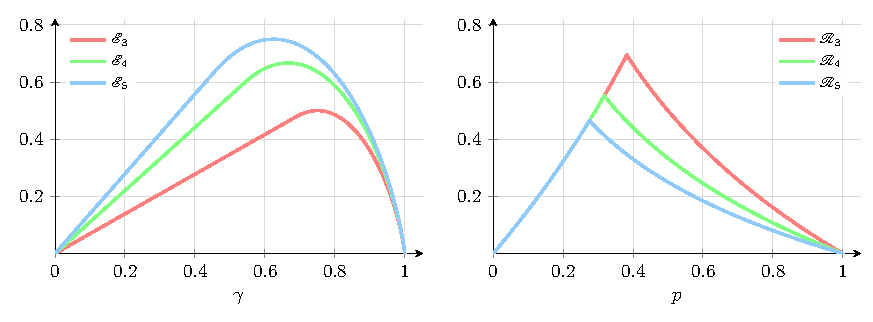
\includegraphics{Graphics/rate-functions.pdf}
	\end{center}
	\caption{The entropy density $\sE_k$ (left) and rate function $\sR_k$ (right) for $k=3,4,5$. The curves $\sR_3$, $\sR_4$, and $\sR_5$ coincide on the interval $[0,p_5]$.}
	\label{fig:rate-funcs}
\end{figure}

The most important feature of both \Cref{thm:main-entropy,thm:main-rate} is that the entropy density and rate function are given by piecewise formulas, reflecting that there are competing structural mechanisms that determine the exponential rates. These competing structures were heuristically described above by noting that the entropy densities or rate functions match the formulas given in $\sE_k$ and $\sR_k$. Our next set of results show that, in fact, these heuristics precisely characterize the typical structure of the corresponding random graph models.

Here and throughout, \emph{almost all} and \emph{almost every} mean all but a $o(1)$ fraction.

\begin{theorem}\label{thm:main-almostall}
Fix $k\geq3$. The following hold:
\begin{enumerate}[
  label=\textit{(\roman*)},
  ref=(\textit{\roman*}),
  topsep=5pt
]
	\item\label{item:thm:main-almostall-super} Fix $\gamma\in(\gamma_k,1)$. If $m\sim\gamma\binom{n}{2}$ then almost every $G\in\cF^\ast_{n,m}(K_{1,k})$ is co-$(k-1)$-partite.
	\item\label{item:thm:main-critical} Let $a_\ast:=\frac{(k-2)p_k(1-p_k)\ln2}{(k-1)\gamma_k}$ and fix $a\in\R$. Let
	$$\gamma:=\gamma_k+a\frac{\log n}{n}$$
	and set $m:=\floor{\gamma\binom n2}$. If $a\leq a_\ast$ then almost every $G\in\cF^\ast_{n,m}(K_{1,k})$ is the disjoint union of two graphs $G=G_1\sqcup G_2$ such that $G_1$ is co-$(k-1)$-partite and
	$$v(G_2)=\left(\frac{a_\ast-a}{2\gamma_k}+o(1)\right)\log n\,.$$
	If $a>a_\ast$ then almost every $G\in\cF^\ast_{n,m}(K_{1,k})$ is co-$(k-1)$-partite.
	\item\label{item:thm:main-almostall-sub} Fix $\gamma\in(0,\gamma_k)$. If $m\sim\gamma\binom{n}{2}$ then almost every $G\in\cF^\ast_{n,m}(K_{1,k})$ is the disjoint union of two graphs $G=G_1\sqcup G_2$ such that $G_1$ is a co-$(k-1)$-partite graph on
	$$(1+o(1))\left(\frac{\gamma(k-1)}{1+(k-2)p_k}\right)^{1/2}n\,,$$
	vertices and $G_2$ is a graph with $\Omega(n)\leq e(G_2)\leq o(n^2)$ edges.
\end{enumerate}
\end{theorem}

For $\gamma\in(\gamma_k,1)$, \Cref{thm:main-almostall} \ref{item:thm:main-almostall-super} significantly strengthens \Cref{thm:main-entropy} since it gives the first-order asymptotics of $N^\ast_{n,m}(K_{1,k})$: letting $r=k-1$ and assuming $r\mid n$, the number $C^r_{n,m}$ of co-$r$-partite graphs on $n$ vertices and $m\sim\gamma\binom{n}{2}$ edges is
$$C^r_{n,m}=(1+o(1))\vast(\sum_{\substack{z_1,\dots,z_r\in\mathbb Z\\ z_1+\cdots+z_r=0}}
\left(\frac{r\gamma-1}{r-1}\right)^{\frac12(z_1^2+\cdots+z_r^2)}\vast)\,\frac{1}{r!}\,
\binom{n}{\frac{n}{r},\dots,\frac{n}{r}}
\binom{\binom{r}{2}\frac{n^2}{r^2}}{\,m-r\binom{n/r}{2}}\,.$$
Meanwhile, in the subcritical regime in \Cref{thm:main-almostall} \ref{item:thm:main-almostall-sub}, there is a nonempty \emph{sparse} remainder on $\Theta(n)$ vertices outside the co-$(k-1)$-partite core.

The next main result describes the typical structure of the conditioned \erdosrenyi{} random graph $G(n,p)$ for constant $p$, where we again observe a structural dichotomy.

\begin{theorem}\label{thm:gnp-typ-struc}
Fix constants $k\geq3$ and $p\in(0,1)$. Let $G$ be the \erdosrenyi{} random graph $G(n,p)$ conditional on the event $G\in\cF^\ast_n(K_{1,k})$. Then the following hold:
\begin{enumerate}[
  label=\textit{(\roman*)},
  ref=(\textit{\roman*}),
  topsep=5pt
]
	\item If $p\in(p_k,1)$ then with high probability $G$ is co-$(k-1)$-partite and
	$$e(G)=(1+o(1))\left(p+\frac{1-p}{k-1}\right)\binom{n}{2}\,.$$
	\item If $p\in(0,p_k]$ then with high probability $G$ has $o(n^2)$ edges.
\end{enumerate}
\end{theorem}

We give intuition further below for the subcritical behavior in \Cref{thm:gnp-typ-struc}. First, we describe the graphon variation problems and their solutions in more detail. Formally, a \emph{graphon} is a symmetric Lebesgue-measurable function $W:[0,1]^2\to[0,1]$, where symmetric means $W(x,y)=W(y,x)$ for all $x,y\in[0,1]$. For background on graphons, we refer the reader to \cite{lovasz2006limits,borgs2008convergent,lovasz2012large}. The set of all graphons is denoted $\cW$. Two graphons $W_1$ and $W_2$ are \emph{equivalent} if there exist measure-preserving maps $\sigma_1,\sigma_2:[0,1]\to[0,1]$ such that $W_1(\sigma_1(x),\sigma_1(y))=W_2(\sigma_2(x),\sigma_2(y))$ almost everywhere. Statements below about the uniqueness of graphons are meant up to this notion of equivalence.

For all $k\geq3$ and $\gamma\in(0,1)$, define the variational problem over graphons $W\in\cW$
\begin{equation}\label{eqn:var-prob-intro-gamma}
\arraycolsep=3pt
\begin{array}[t]{lll}
\Phi_k(\gamma) \hspace{0.5mm}:= & \sup & \displaystyle\int_{[0,1]^2}H(W(x,y)) \, dx \, dy \\[16pt]
&\text{s.t.} & \displaystyle\int_{[0,1]^{k+1}}\Bigg(\prod_{i=2}^{k+1}W(x_1,x_i)\Bigg)\Bigg(\prod_{2\leq i<j\leq k+1}(1-W(x_i,x_j))\Bigg) \prod_{i=1}^{k+1}dx_i = 0 \,, \\[22pt]
&& \displaystyle\int_{[0,1]^2}W(x,y) \, dx \, dy=\gamma \,.
\end{array}
\end{equation}
The first constraint states that $W$ has zero $K_{1,k}$ density, or equivalently, for the familiar reader, that the $W$-random graph $G(n,W)$ is induced-$K_{1,k}$-free with probability 1. The second constraint states that $W$ has edge density $\gamma$.

\begin{theorem}\label{thm:ent-graphons}
Fix $k\geq3$. For all $\gamma\in[\gamma_k,1)$, $\Phi_k(\gamma)$ has a unique optimizer up to equivalence, while for all $\gamma\in(0,\gamma_k)$, there are infinitely many non-equivalent optimizers.
\end{theorem}

Next, we state the solution to the variational problem for the conditioned \erdosrenyi{} random graph. For $p\in(0,1)$, define the relative entropy
\begin{equation}\label{eqn:rel-ent-dfn}
I_p(x):=x\log\frac{x}{p}+(1-x)\log\frac{1-x}{1-p}\,.
\end{equation}
For all $k\geq3$ and $p\in(0,1)$, define the variational problem over graphons $W\in\cW$
\begin{equation}\label{eqn:var-prob-intro-p}
\arraycolsep=3pt
\begin{array}[t]{lll}
\Psi_k(p) \hspace{0.5mm}:= & \inf & \displaystyle\int_{[0,1]^2}I_p(W(x,y)) \, dx \, dy \\[16pt]
&\text{s.t.} & \displaystyle\int_{[0,1]^{k+1}}\Bigg(\prod_{i=2}^{k+1}W(x_1,x_i)\Bigg)\Bigg(\prod_{2\leq i<j\leq k+1}(1-W(x_i,x_j))\Bigg) \prod_{i=1}^{k+1}dx_i = 0 \,.
\end{array}
\end{equation}

\begin{theorem}\label{thm:gnp-graphons}
Fix $k\geq3$. For all $p\in(0,p_k)$, the unique optimizer of $\Psi_k(p)$, up to equivalence, is the all-zero graphon; for $p=p_k$, there are infinitely many non-equivalent optimizers; and for $p\in(p_k,1)$, there is again a unique optimizer up to equivalence.
\end{theorem}

To understand heuristically why the all-zero graphon is the subcritical optimizer in \Cref{thm:gnp-graphons}, consider that the rate function for induced-$K_{1,k}$-freeness in $G(n,p)$ can be written as an infimum over fixed edge densities $\gamma\in(0,1)$. For all $\gamma$, \Cref{thm:main-almostall} implies that for the uniformly random graph $G\in\cF^\ast_{n,m}(K_{1,k})$ with $m\sim\gamma\binom{n}{2}$, with high probability there is a partition of $V(G)$ into parts of size $\Theta(n)$ whose internal and between-part densities are either $o(1)$, $1-o(1)$, or some $p_\gamma+o(1)\geq p_k$. Hence, if $p<p_k$ then there is no optimizer of $\Phi_k(\gamma)$ that takes the value $p$ anywhere. But since the relative entropy $I_p(x)$ is uniquely minimized at $x=p$, this means no fixed-density optimizer of $\Phi_k(\gamma)$ for $\gamma\in(0,1)$ can also be an optimizer of $\Psi_k(p)$ whenever $p<p_k$, leaving only the all-zero graphon.

\begin{figure}
	\begin{center}
	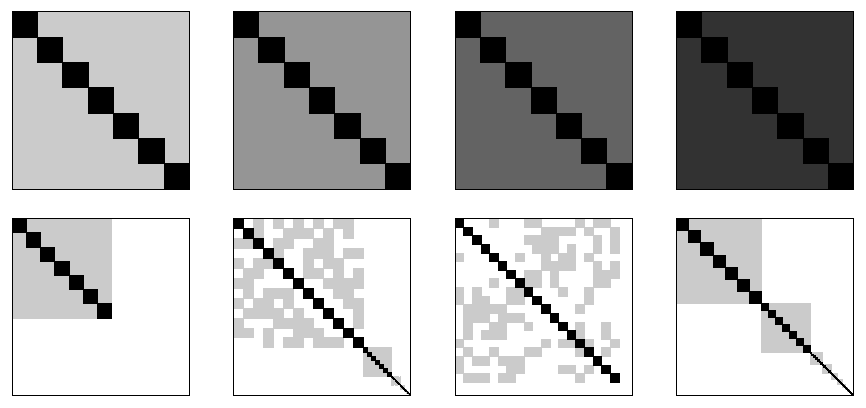
\includegraphics{Graphics/graphons.pdf}
	\end{center}
	\caption{Optimal graphons for induced-$K_{1,8}$-free graphs of fixed edge density. The top row shows the unique optimal graphons of edge densities $\gamma_8\approx0.317$, $\frac{1}{2}$, $\frac{2}{3}$, and $\frac{5}{6}$. The bottom row shows examples of optimal graphons of edge density $\frac{1}{10}$. The white areas represent density 0, gray areas density $p_\gamma\in(0,1)$, and black areas density 1.}
	\label{fig:graphons}
\end{figure}

The next theorem shows that the induced-$H$-free fixed-density variational problem does \emph{not} necessarily exhibit a phase transition for general $H$. A graph $G$ is a \emph{split graph} if there is a partition $V(G)=A\cup B$ such that $G[A]$ is an independent set and $G[B]$ is a clique.

\begin{theorem}\label{thm:c4-main}
Fix a constant $\gamma\in(0,1)$ and let $m\sim\gamma\binom{n}{2}$. Almost all induced-$C_4$-free graphs on $n$ vertices and $m$ edges are split graphs. In particular,
\begin{equation}\label{eqn:c4-entropy-main}
\lim_{n\to\infty}\frac{1}{\binom{n}{2}}\log N^\ast_{n,m}(C_4)=\max_{\lambda\in[0,1]}\left\{2\lambda(1-\lambda)\,H\!\left(\frac{\gamma-\lambda^2}{2\lambda(1-\lambda)}\right)\right\}\,,
\end{equation}
where the maximum is over $\lambda$ for which the right-hand side is well-defined.
\end{theorem}

The right-hand side of \eqref{eqn:c4-entropy-main} is an analytic function of $\gamma\in(0,1)$, reflecting the absence of a phase transition. \Cref{thm:c4-main} resolves the dense case of a conjecture of \citeauthor{morris2024asymmetric} \cite[Conjecture~6.1]{morris2024asymmetric} and refines the theorem of \citeauthor{promel1991excluding} \cite{promel1991excluding} stating that almost all induced-$C_4$-free graphs are split graphs.

\subsection{Overview of proofs}\label{subsec:overview}
Our starting point is the graphon variational problem \eqref{eqn:var-prob-intro-gamma}. We solve \eqref{eqn:var-prob-intro-gamma} via a reduction to an extremal problem over 3-edge-colored graphs. This extremal problem is closely related to prior literature discussed in \Cref{subsec:edit-distance}. We summarize the reduction here.

First, \Cref{lemma:UFHatGraphonSeq} shows that a graphon that is feasible for \eqref{eqn:var-prob-intro-gamma} is the limit of a sequence of \emph{types} $T$ of induced-$K_{1,k}$-free graphs. A type is an $\epsilon$-regular partition equipped with a 2-vertex-colored, 3-edge-colored graph $J$ that encodes whether clusters and pairs of clusters have density close to 0 (green), 1 (blue), or an intermediate value (red). If $T$ is a type for an induced-$K_{1,k}$-free graph, then the induced embedding lemma implies there is no induced homomorphism from $K_{1,k}$ into $J$, written $K_{1,k}\nHookrightarrow J$. If $0\leq d_{ij}\leq1$ represents the density between clusters $i$ and $j$ for all $1\leq i<j\leq\ell$, then the number of induced-$K_{1,k}$-free graphs of edge density $\gamma+o(1)$ that are consistent with $T$ and $\{d_{ij}\}_{1\leq i<j\leq\ell}$ is $e^{o(n^2)}\prod_{i<j}\binom{(n/\ell)^2}{d_{ij}(n/\ell)^2}$. For a fixed type $T$, if the logarithm of this quantity is near-maximum then concavity of the entropy implies the densities $d_{ij}$ corresponding with red pairs $ij$ are nearly equal to one another. The common value of these $d_{ij}$ is $(\gamma\binom{\ell}{2}-e_\blue(J))/e_\red(J)+o(1)$, where $e_\red(J)$ and $e_\blue(J)$ are the numbers of red and blue edges of $J$, respectively.

This motivates the following finite objective. For a 3-edge-colored graph $J$ on $\ell$ vertices with $e_\red(J)>0$, define
\begin{equation}\label{eqn:overview-fgamma}
f_\gamma(J):=e_\red(J)\cdot H\!\left(\frac{\gamma\binom{\ell}{2}-e_\blue(J)}{e_\red(J)}\right)\,.
\end{equation}
Up to the normalizing factor $2/\ell^2$ and a $o(1)$ error, the entropy contribution of a type with colored graph $J$ is governed by $f_\gamma(J)$. Consequently, solving the graphon variational problem reduces to proving extremal and stability results for $f_\gamma(J)$ over colored graphs $J$ satisfying $K_{1,k}\nHookrightarrow J$.

For excluded induced stars, we first prove stability for the linear extremal inequality
\begin{equation}\label{eqn:overview-ineq}
e_\red(J)\leq (k-2)e_\blue(J)+O_k(\ell)\,.
\end{equation}
That is, we prove that every $J$ with $K_{1,k}\nHookrightarrow J$ satisfies \eqref{eqn:overview-ineq} and, moreover, every $J$ for which \eqref{eqn:overview-ineq} is met with near equality is close in Hamming distance to an explicit extremal structure. Passing back to graphons, this gives the constraint $|R_W|\leq (k-2)|O_W|$, where $R_W=\{0<W<1\}$ and $O_W=\{W=1\}$. Jensen's inequality then reduces \eqref{eqn:var-prob-intro-gamma} to a two-variable calculus problem in $|R_W|$ and $|O_W|$, whose solution is $\sE_k(\gamma)$, and whose optimizers satisfy $|R_W|=(k-2)|O_W|$. The proofs of \eqref{eqn:overview-ineq} and the stability of the extremal structure use symmetrization, a local \erdos{}--Simonovits stability step, and an iterative extraction of reduced $(k-2)$-regular components. The extremal structure for \eqref{eqn:overview-ineq} is reflected in the graphons in \Cref{fig:graphons}. For induced-$C_4$-free graphs, we directly prove stability of the objective $f_\gamma(J)$ for every fixed $\gamma\in(0,1)$; in this case, the stable extremal structures are split colorings.

The entropy density and rough structure of fixed-density induced-$H$-free graphs follow from the solution to the graphon variational problem. The finer typical structure assertions require estimates beyond the leading entropy. For excluded induced stars, we first choose a vertex partition minimizing the number of edits needed to obtain the prescribed structure, following the counting approach of \cite{balogh2020efficient,perkins2025typical}. Missing edges inside clique parts and edges between parts that should be nonadjacent are called \emph{defects}. We bound the number of graphs with defects and then compare the counts for the remaining candidate structures.

In \Cref{sec:supercritical}, the partition consists of $k-1$ main parts and a remainder. Optimality excludes high defect degrees. A vertex of intermediate defect degree gives many potential induced stars, whose exclusion incurs a factor $e^{-cn^2}$. When all defect degrees are small, a matching of $h$ defects gives a factor $e^{-chn}$. Janson's inequality supplies these bounds, which outweigh the choices of defects. Holding the remainder graph fixed, we therefore compare with graphs in which the main parts are cliques and have no edges to the remainder. Above $\gamma_k$, absorbing a remainder of size $s$ into a main part increases the count by a factor at least $e^{csn}$. This outweighs the choices of the remainder vertices and proves that almost every graph is co-$(k-1)$-partite.

At the critical density, the linear term in the completion-count comparison vanishes, and the second-order term becomes decisive. In \Cref{sec:critical}, we use the same defect estimates and count the remaining graphs according to their remainder size $s$. For $\gamma=\gamma_k+a\log n/n$ and $s=O(\log n)$, the base-2 logarithm of this count relative to the co-$(k-1)$-partite count is
$$\left(1-\frac{a}{a_\ast}\right)s\log n-\frac{\gamma_k}{a_\ast}s^2+o((\log n)^2)\,,$$
where $a_\ast$ is as in \Cref{thm:main-almostall} \ref{item:thm:main-critical}. Choosing the remainder vertices supplies the $s\log n$ term, while a second-order expansion of the binomial completion count supplies the other two terms. The rate function controls the weighted count of graphs inside the remainder. A quadratic tail bound excludes larger remainders, and maximizing the displayed expression gives the asserted first-order asymptotics. Above $a_\ast$, a further comparison for small positive $s$ shows that the remainder is empty with high probability.

In \Cref{sec:subcritical}, the optimal graphon may have many components. We retain a finite collection of components carrying all but a small amount of the edge density and include the others in the remainder. A \emph{profile} records the local neighborhood data of vertices with many defects and the matching number of the remaining defect graph. If a vertex is adjacent to an intermediate fraction of one part, it must be adjacent to almost all of a neighboring part in the reduced graph. Induced-star-freeness also bounds the number of parts in which the vertex has substantial degree. These restrictions let the losses from almost-complete neighborhoods compensate for the choices of intermediate-density neighborhoods. Combining the edge-count comparison with binomial tail estimates gives a uniform loss per exceptional vertex; in the only configuration where this bound could be tight, optimality of the partition forces a strictly positive relative-entropy loss. The remaining defects have small degrees and are handled by the matching argument and Janson's inequality.

To select the typical subcritical optimizer, we compare these counts with those near the one-component graphon $W^\ast$ on the lower-left of \Cref{fig:graphons}. This graphon leaves the most vertices available for the sparse remainder. Any optimizer a fixed positive cut distance away leaves $\Theta(n)$ fewer such vertices in the comparison. On the additional vertices, inserting a matching gives $e^{\Theta(n\log n)}$ choices. The entropy bound makes each candidate core count at most $e^{O(n)}$ times the reference core count. Transferring $O(n)$ edges from the core to the remainder to preserve the total edge count also costs only $e^{O(n)}$, as do the choices of vertex partitions. This proves concentration at $W^\ast$. We then use the defect estimates and control the multiplicity of clique covers to obtain the exact decomposition in \Cref{thm:main-almostall} \ref{item:thm:main-almostall-sub}. A further matching comparison on isolated remainder vertices gives the linear lower bound on its number of edges.

\subsection{Related work}
\subsubsection{Coloring number and criticality.}\label{subsec:col-num}
The \emph{coloring number} $\tau(H)$ is the least integer $q$ such that, for every pair of nonnegative integers $s,t$ with $s+t=q$, the vertices of $H$ can be partitioned into $s$ cliques and $t$ independent sets. For $\tau(H)\geq3$, \citeauthor{balogh2011excluding} \cite{balogh2011excluding} proved a criticality criterion for almost every induced-$H$-free graph to admit a partition into $s$ cliques and $t$ independent sets, where $s+t=\tau(H)-1$ and $H$ admits no such partition. This is the induced analogue of the characterization by \citeauthor{promel1992asymptotic} \cite{promel1992asymptotic} of non-bipartite graphs $H$ for which almost all $H$-free graphs are $(\chi(H)-1)$-partite. These results concern graphs without a prescribed edge count. In the fixed-density setting studied here, even for excluded induced stars, the typical structure depends on the density and can include a nonempty sparse remainder.

\subsubsection{Edit distance and hereditary properties.}\label{subsec:edit-distance}
Our work is related to literature on extremal problems for multigraphs, most notably by \citeauthor{marchant2010extremal} \cite{marchant2010extremal,marchant2011structure} and \citeauthor{thomason2011graphs} \cite{thomason2011graphs}. This literature focuses on calculating an extremal parameter $\kappa_p$ that is analogous to the Tur\'an density. Theorem 4.4 in \cite{marchant2010extremal} shows how to convert between $\kappa_p$ and the large deviation rate function for a hereditary property in $G(n,p)$. Consequently, these results determine the large deviation rate function for induced-$H$-freeness for several specific graphs $H$. For excluded induced stars, \citeauthor{thomason2011graphs} \cite[Section~7.5]{thomason2011graphs} exhibits infinitely many colored extremal structures at $p=p_k$, consistent with the graphon optimizer family in \Cref{thm:gnp-graphons}. Our work differs from this previous literature in that we focus mainly on the fixed-density setting, characterize all graphon optimizers for both models, and prove finer typical structure results.

\subsubsection{Other density-constrained models}
Numerous prior works have studied typical structure and phase transitions in random graph models defined by subgraph density constraints. A well-studied case is the uniformly random graph of given edge and triangle density; several works have characterized optimal graphons in subsets of the feasible region of densities and proven the existence of phase transitions \cite{radin2013phase,radin2014asymptotics,radin2015singularities}. The main variational problem studied here imposes zero induced-star density. Allowing a small positive induced-star density leads to the question in \Cref{conj:relaxed-star-exclusion}: whether this relaxation selects the same one-component graphon as the lower-order counting argument, despite the existence of infinitely many optimizers under exact exclusion.

\subsection{Future directions}
A natural extension is to allow a small positive density of induced stars. For $k\geq3$, $\gamma\in(0,1)$, and $\epsilon\geq0$, define
$$\Phi_k(\gamma,\epsilon):=\sup\left\{H(W):W\in\cW\,,\,t(K_2,W)=\gamma\,,\,t_\ind(K_{1,k},W)\leq\epsilon\right\}\,,$$
where $H(W):=\int_{[0,1]^2}H(W(x,y))\,dx\,dy$. Our results give $\Phi_k(\gamma,0)=\sE_k(\gamma)$ and infinitely many optimizers when $\gamma<\gamma_k$. We conjecture that allowing a vanishing induced-star density selects the same one-component graphon as the finite counting argument.

For $\gamma\in(0,\gamma_k)$, put $\mu:=\sqrt{\gamma/\gamma_k}$ and $s:=1-\mu$. Let $W^\ast$ be the graphon obtained by rescaling $W^\ast_{\gamma_k}$ from \eqref{eqn:opt-graphon-super} to $[0,\mu]^2$ and setting it equal to zero elsewhere.

\begin{conjecture}\label{conj:relaxed-star-exclusion}
Fix $k\geq3$ and $\gamma\in(0,\gamma_k)$. As $\epsilon\downarrow0$,
$$\Phi_k(\gamma,\epsilon)=\sE_k(\gamma)+\left(\frac{s^{(k-1)/k}}{k}+o(1)\right)\epsilon^{1/k}\log\frac1\epsilon\,.$$
Moreover, every choice of optimizing graphons $W_\epsilon$ satisfies
$$\delta_\square(W_\epsilon,W^\ast)\longrightarrow0\,.$$
\end{conjecture}

The proposed entropy correction is attained to leading order by putting a small constant density $q$ on the isolated remainder of $W^\ast$ and shrinking its nonzero component to preserve edge density $\gamma$. The induced-star density is then asymptotic to $s^{k+1}q^k$, while the entropy gain is $s^2q\log(1/q)+O_{k,\gamma}(q)$. The conjecture concerns the leading correction and limiting graphon, rather than the exact form of an optimizer for positive $\epsilon$; smaller perturbations inside the clique parts may further increase the entropy.

\subsection{Organization}
In \Cref{sec:prelim}, we include background on colored graphs, regularity, graphons, and cut metric that will be used throughout the paper. In \Cref{sec:graphon-prob}, we solve the graphon variational problems, fully characterizing all optimizers. In \Cref{sec:entropy} we prove \Cref{thm:main-entropy,thm:main-rate,thm:ent-graphons,thm:gnp-graphons}. In \Cref{sec:supercritical,sec:critical,sec:subcritical}, we prove \Cref{thm:main-almostall} \ref{item:thm:main-almostall-super}, \ref{item:thm:main-critical}, and \ref{item:thm:main-almostall-sub}, respectively. In \Cref{sec:erdosrenyi}, we prove \Cref{thm:gnp-typ-struc}. In \Cref{sec:edge-coloring}, we establish the extremal and stability results for edge colorings that underlie the graphon analysis. In \Cref{sec:deferred}, we give deferred proofs from the earlier sections. Finally, in \Cref{sec:c4-free} we prove \Cref{thm:c4-main}.


\section{Preliminaries}
\label{sec:prelim}
\subsection{Notation}
We will write both $V(K_n)$ and $V$ for a vertex set of size $n$. The complement of a set or graph $X$ is denoted $X^c$. The base-2 logarithm is denoted $\log$ and the natural logarithm is denoted $\ln$. Induced subgraph containment is denoted $H\leq G$. For subsets $A,B\subseteq V$, we write $G[A,B]$ for the graph on $A\cup B$ containing all edges of $G$ with one endpoint in $A$ and another in $B$. To emphasize the underlying graph $G$, we write $e_G(\cdot)$, $d_G(\cdot)$, $N_G(\cdot)$, etc. We use the superscript $c$ to denote neighborhood and degree in the complementary graph $G^c$; for example, $N^c(v)=V\setminus(N(v)\cup\{v\})$, $N^c(v,A):=N^c(v)\cap A$, $d^c(v):=|N^c(v)|$, and $d^c(v,A):=|N^c(v,A)|$. For vertices $i,j$ we use the shorthand $ij:=\{i,j\}$. If $\cH$ is a collection of graphs then we write $\cH(n)$ for the set of $H\in\cH$ on $n$ vertices; conversely, if $\cH(n)$ is defined for various $n$ then we write $\cH:=\bigcup_{n\geq1}\cH(n)$.

\subsection{Janson's inequality}
The following version of Janson's inequality due to \citeauthor{riordan2015janson} \cite{riordan2015janson} applies to families of events that are positively correlated and plays an important role in this paper. On several occasions, we will define a family of copies of $K_{1,k}$ and use \Cref{thm:JansonsInequality} to bound the probability that none of these copies appears in a random graph.

\begin{theorem}[\normalfont{\cite{riordan2015janson}}]\label{thm:JansonsInequality}
Let $(\Omega,\cF,\bbP)$ be a probability space. Let $\cI\subseteq\cF$ be a family of events such that for all $A,B\in\cI$ we have $\bbP\{A\cap B\}\geq\bbP\{A\}\bbP\{B\}$, $A\cap B\in\cI$, and $A\cup B\in\cI$. Let $B_1,\dots,B_n\in\cI$ and define
$$\mu:=\sum_{i=1}^n\bbP\{B_i\}\hspace{7mm}\text{and}\hspace{7mm}\Delta:=\sum_{i\sim j}\bbP\{B_i\cap B_j\}\,,$$
the second sum being over unordered pairs $i\neq j$ such that $B_i$, $B_j$ are not independent. If $\mu>0$ then
$$\bbP\!\left\{\bigcap_{i=1}^nB_i^c\right\}\leq\exp\!\left(-\min\left\{\frac{\mu}{2}\,,\,\frac{\mu^2}{4\Delta}\right\}\right)\,.$$
Here the quotient is interpreted as $+\infty$ when $\Delta=0$; in that case the stronger bound $e^{-\mu}$ holds. If $\mu=0$ the trivial bound $1$ applies.
\end{theorem}
For independent Bernoulli coordinates, the increasing events satisfy these hypotheses. Mixed edge/nonedge events may therefore be used whenever one common complementation of coordinates makes every event increasing; the orientation must be consistent across the entire family.

\subsection{Colored homomorphisms}\label{subsec:colored-graphs}
Graph regularity and induced embeddings are important tools in our proofs. It is convenient and standard \cite{marchant2010extremal,marchant2011structure,bottcher2012perfect,martin2013edit} to work with vertex- and edge-colored graphs that encode which induced subgraphs can be embedded into a regular partition. We first introduce colored graphs and homomorphisms in this subsection, and then their applications to our setting in \Cref{subsec:regularity}.

A \emph{colored graph} $J=(F,\sigma)$ is a graph $F$ with a 3-coloring $\sigma:V(F)\cup E(F)\to\{\red,\green,\blue\}$ of its vertices and edges such that $\sigma(V(F))\subseteq\{\green,\blue\}$. We write $V(J):=V(F)$ and $E(J):=E(F)$. Let $G$ be a graph and $J$ a colored graph. A \emph{colored homomorphism} from $G$ to $J$ is a mapping $\phi:V(G)\to V(J)$ such that the following conditions hold:
\begin{enumerate}[
  label=\textit{(\roman*)},
  ref=(\textit{\roman*}),
  topsep=5pt
]
    \item If $ij\in E(G)$ and $\phi(i)\neq\phi(j)$ then $\phi(i)\phi(j)\in E(J)$.
    \item If $uv\in E(G)$ then either $\phi(u)\neq\phi(v)$ and $\sigma(\phi(u)\phi(v))\in\{\red,\blue\}$, or $\phi(u)=\phi(v)$ and $\sigma(\phi(u))=\blue$.
    \item If $uv\not\in E(G)$ then either $\phi(u)\neq\phi(v)$ and $\sigma(\phi(u)\phi(v))\in\{\green,\red\}$, or $\phi(u)=\phi(v)$ and $\sigma(\phi(u))=\green$.
\end{enumerate}
In other words, edges (and only edges) are embedded into \blue, non-edges (and only non-edges) are embedded into \green, and both can be embedded into \red. We write $G\hookrightarrow J$ if there exists a colored homomorphism from $G$ to $J$. For example, $C_4\hookrightarrow\grg$ and $K_{1,3}\hookrightarrow\exampletriangle$.

Let $\cC(n)$ be the set of colored graphs on $n$ vertices, and let
$$\cC(n,G):=\{J\in\cC(n):G\nHookrightarrow J\}\,.$$
An \emph{edge-colored graph} $J=(F,\tau)$ is a graph $F$ with a 3-coloring $\tau:E(F)\to\{\red,\green,\blue\}$ of its edges. Again, we write $V(J):=V(F)$ and $E(J):=E(F)$.

\subsection{Graph regularity}\label{subsec:regularity}
Here we introduce \emph{types}, which are regularity graphs used for subgraph embedding. We mostly follow the framework of \citeauthor{bottcher2012perfect} \cite{bottcher2012perfect}. To simplify the exposition, we instead directly define a type as a structure that satisfies the conclusions of the induced embedding lemma \cite[Lemma~2.9]{bottcher2012perfect}. In analogy with the regularity lemma, the results of \cite{bottcher2012perfect} imply such a structure always exists, as we show in \Cref{lemma:type-lemma}.

A pair $A,B\subseteq V(G)$ is \emph{$\epsilon$-regular} in a graph $G$ if for all $A'\subseteq A$ and $B'\subseteq B$ such that $\abs{A'}\geq\epsilon\abs{A}$ and $\abs{B'}\geq\epsilon\abs{B}$, $\abs{d(A',B')-d(A,B)}\leq\epsilon$, where $d(X,Y):=\frac{e(X,Y)}{|X|\cdot|Y|}$. An \emph{$\epsilon$-regular partition} of $G$ is a partition $V(G)=V_0\cup V_1\cup\cdots\cup V_k$ such that $\abs{V_1}=\cdots=\abs{V_k}$, $\abs{V_0}\leq\epsilon\abs{V(G)}$, and all but at most $\epsilon\binom{k}{2}$ of the pairs $1\leq i<j\leq k$ are $\epsilon$-regular.

\begin{definition}[Type]\label{dfn:type}
Let $G$ be a graph on $n$ vertices, and let $\epsilon,\delta\in(0,\frac{1}{2})$ and $\ell\in\N$. An \emph{$(\epsilon,\delta,\ell)$-type} for $G$ is a pair $(P,R)$ where $P=\{V_0,V_1,\dots,V_k\}$ is an $\epsilon$-regular partition of $G$ and $R=([k],E_R,\sigma)$ is a colored graph such that the following conditions hold:
\begin{enumerate}[
  label=\textit{(\roman*)},
  ref=(\textit{\roman*}),
  topsep=5pt
]
    \item For all $1\leq i<j\leq k$, $ij\in E_R$ if and only if $\{V_i,V_j\}$ is $\epsilon$-regular in $G$.
    \item For all $ij\in E_R$, we have $\sigma(ij)=\green$ if $d(V_i,V_j)<\delta$; $\sigma(ij)=\red$ if $d(V_i,V_j)\in[\delta,1-\delta]$; and $\sigma(ij)=\blue$ if $d(V_i,V_j)>1-\delta$.
    \item\label{item:type-colored-homo} If $H$ is a graph on at most $\ell$ vertices and $H\hookrightarrow R$ then $H\leq G$.
\end{enumerate}
If all the above conditions hold then we say $G$ \emph{has} type $(P,R)$.
\end{definition}


\subsection{Graphons and entropy}\label{subsec:graphons}
The \emph{entropy} of a graphon $W\in\cW$ is defined as
$$H(W):=\int_{[0,1]^2}H(W(x,y))\,dx\,dy\,,$$
and for all $p\in[0,1]$, the \emph{relative entropy} of $W$ is defined as
$$I_p(W):=\int_{[0,1]^2}I_p(W(x,y))\,dx\,dy\,,$$
The following lemmas, which are \cite[Propositions~2.10~\&~2.11]{perkins2025typical}, state that the entropy density and rate function for induced-$H$-freeness are given by variational problems over graphons. We write $t_\ind$ and $t$ for the induced and non-induced homomorphism densities; these are written explicitly in \eqref{eqn:var-prob-intro-gamma} in the case of $K_{1,k}$ and $K_2$, and we refer the reader to \cite{lovasz2012large} for the general definition. We also define
$$\rand(W):=\abs{\{(x,y)\in[0,1]^2:0<W(x,y)<1\}}\,.$$

\begin{lemma}\normalfont{(\cite{perkins2025typical})}\label{lemma:LDPforGNPkl}
Let $p\in(0,1)$ be a constant and $G\sim G(n,p)$. If $H$ is a fixed graph and
$$\cF:=\{W\in\cW:t_{\ind}(H,W)=0,\,\rand(W)>0\}$$
is nonempty then
$$\lim_{n\to\infty}\frac{1}{\binom{n}{2}}\log\bbP\{G\in\cF^\ast_n(H)\}=-\inf_{W\in\cF}I_p(W)\,.$$
\end{lemma}
The infimum is unchanged if the condition $\rand(W)>0$ is omitted. Indeed, fix $V\in\cF$ and any induced-$H$-free graphon $U$. Put copies of $U$ and $V$ on blocks of lengths $1-a$ and $a$, respectively, with cross value zero if $H$ is connected and one otherwise. In the latter case $H^c$ is connected, so the resulting graphon $U_a$ is induced-$H$-free in either case. Also $\rand(U_a)\geq a^2\rand(V)>0$ and $I_p(U_a)\to I_p(U)$ as $a\downarrow0$ by the two-block integral formula. This proves the equality of the two infima.

\begin{lemma}\normalfont{(\cite{perkins2025typical})}\label{lemma:FnmGraphonOptAsymps}
Let $\gamma\in(0,1)$, $n,m\in\N$, and $m\sim\gamma\binom{n}{2}$. If $H$ is a fixed graph and
$$\cF_\gamma:=\{W\in\cW:t(K_2,W)=\gamma,\,t_{\ind}(H,W)=0,\,\rand(W)>0\}$$
is nonempty then
$$\lim_{n\to\infty}\frac{1}{\binom{n}{2}}\log|\cF^\ast_{n,m}(H)|=\sup_{W\in\cF_\gamma}H(W)\,.$$
\end{lemma}

We now define graphons naturally associated to matrices, graphs, and types. For integers $i,j\in[n]$, define
\begin{equation}\label{dfn:snij}
S^n_{ij}:=\left(\frac{i-1}{n},\frac{i}{n}\right)\times\left(\frac{j-1}{n},\frac{j}{n}\right)\cup\left(\frac{j-1}{n},\frac{j}{n}\right)\times\left(\frac{i-1}{n},\frac{i}{n}\right)\subseteq[0,1]^2\,.
\end{equation}
For a symmetric matrix $M\in\R^{n\times n}$, the graphon $W_M$ associated to $M$ is defined as
$$W_M:=\sum_{1\leq i\leq j\leq n}M_{ij}\,\bsone_{S_{ij}^n}\,.$$
If $G$ is either an unweighted or weighted graph on $n$ vertices with adjacency or weight matrix $A$ then we define the graphon $W_G:=W_A$.
If a graph $G$ has the $(\epsilon,\delta,\ell)$-type $T=(P,R)$, where $P=\{V_0,V_1,\dots,V_k\}$, then the graphon $W_T$ associated with $T$ and $G$ is defined by
$$W_T:=\sum_{1\leq i\leq j\leq k}d_G(V_i,V_j)\,\bsone_{S_{ij}^k}\,.$$
Note that the exceptional set $V_0$ is not represented in the graphon $W_T$.

The cut metric and related notions of distance between graphons are important tools in this paper. We record the necessary definitions here and refer the reader to \cite{lovasz2012large} for more details. The \emph{cut norm} of a graphon $W\in\cW$ is defined as
$$\norm{W}_\square:=\sup_{S,T\subseteq[0,1]}\bigg|\int_{S\times T}W(x,y)\,dx\,dy\bigg|\,.$$
For a graphon $W\in\cW$ and a map $\varphi:[0,1]\to[0,1]$, define the graphon $W^\varphi$ by $W^\varphi(x,y)=W(\varphi(x),\varphi(y))$. The \emph{cut metric} is a distance between graphons $W,W'\in\cW$ defined as
$$\delta_\square(W,W'):=\inf_\varphi\,\norm{W^\varphi-W'}_\square\,,$$
where the infimum is over measure-preserving bijections $\varphi$. The cut metric $\delta_\square$ is defined on pairs of graphons, (weighted or unweighted) graphs, and matrices, and any combination thereof by using the corresponding graphon associated to those objects (i.e.\ $W_G$ or $W_M$). The \emph{cut norm} of a real $n\times n$ matrix $A$ is defined as
$$\norm{A}_\square:=\frac{1}{n^2}\,\max_{S,T\subseteq[n]}\Bigg|\sum_{i\in S,j\in T}A_{ij}\Bigg|\,.$$
For weighted graphs $G$ and $H$ on $n$ vertices with adjacency matrices $A_G$ and $A_H$, we define the two notions of distance
\begin{align*}
d_\square(G,H) &:= \norm{A_G-A_H}_\square \,, \\[3pt]
\widehat{\delta}_\square(G,H) &:= \min_P\,\norm{A_G-P^TA_HP}_\square \,,
\end{align*}
where the minimum is over $n\times n$ permutation matrices. Finally, the \emph{edit distance} between two graphs $G$ and $H$ is defined as
$$d_1(G,H):=\frac{1}{n^2}\,|E(G)\,\triangle\,E(H)|\,,$$
where $\triangle$ is the symmetric difference.

The following lemma plays an important role in the solution to the graphon variational problem in \Cref{sec:graphon-prob}: it allows us to transfer from a graphon $W$ with zero induced $H$ density to a sequence of types that converge to $W$. The lemma is proven in \Cref{sec:deferred}.

\begin{restatable}{lemma}{GraphonSeq}\label{lemma:UFHatGraphonSeq}
Fix a graph $F$. For all $W\in\cW$ such that $t_{\ind}(F,W)=0$ and all $\delta\in(0,1/2)$, there exists a sequence $\{W_m\}_{m\in\N}$ of graphons such that the following conditions hold:
\begin{enumerate}[
  label=\textit{(\roman*)},
  ref=(\textit{\roman*}),
  topsep=5pt
]
	\item $\delta_\square(W_m,W)\to0$ as $m\to\infty$.
    \item There exists a graphon $W'$ such that $\norm{W_m-W'}_1\to0$ as $m\to\infty$.
	\item For all $m$ there exists $\eta_m>0$ such that $W_m$ is the graphon associated with an $(\eta_m,\delta,v(F))$-type $(P_m,R_m)$ of an induced-$F$-free graph.
	\item $\eta_m\to0$ and $v(R_m)\to\infty$ as $m\to\infty$.
\end{enumerate}
\end{restatable}


\section{Solving the Graphon Variational Problem}
\label{sec:graphon-prob}
In this section we solve the variational problems \eqref{eqn:var-prob-intro-gamma} and \eqref{eqn:var-prob-intro-p}. Let $k\geq3$ be an integer fixed throughout this section, and let $\Delta:=k-2$. For all $\gamma\in(0,1)$ define the set of graphons
$$\cX_\gamma:=\{W\in\cW:t_\ind(K_{1,k},W)=0\,,\,t(K_2,W)=\gamma\}\,.$$
Then the variational problems \eqref{eqn:var-prob-intro-gamma} and \eqref{eqn:var-prob-intro-p} can be written
\begin{align}
\Phi_k(\gamma) &= \sup\{H(W):W\in\cX_\gamma\} \,,\label{eqn:var-prob-fixed-gamma} \\[4pt]
\Psi_k(p) &= \inf\{I_p(W):t_\ind(K_{1,k},W)=0\} \,.
\end{align}
Let $\cX_\gamma^\ast$ be the set of optimizers in \eqref{eqn:var-prob-fixed-gamma}, which is nonempty since $\cX_\gamma$ is compact and $H$ is upper semicontinuous in the cut metric topology (see \cite[Theorem~3.7]{borgs2008convergent} and \cite[Lemma~2.1]{chatterjee2011large}).

We now define the set of graphons we will prove are the optimizers in \eqref{eqn:var-prob-fixed-gamma}.
For a graph $G$ on $[n]$, define the function $\xi_G:\R^2\to[0,1]$ by
\begin{equation}\label{eqn:xiG-dfn}
\xi_G(x,y)=\sum_{i=1}^n\bsone_{S^n_{ii}}+\sum_{ij\in E(G)}p_k\,\bsone_{S_{ij}^n}\,,
\end{equation}
where $S_{ij}^n$ is defined in \eqref{dfn:snij}.

Let $\bLambda$ denote the set of all (finite or infinite) sequences $((\lambda_1,G_1),(\lambda_2,G_2),\dots)$ of pairs where the numbers $\lambda_i\in[0,1]$ are strictly increasing in $i\geq1$, the numbers $\lambda_i-\lambda_{i-1}$ are nonincreasing in $i\geq1$ (where $\lambda_0:=0$), and each $G_i$ is a connected $\Delta$-regular graph. For all $\blambda=((\lambda_i,G_i))_{i\geq1}\in\bLambda$ define the graphon $W_\blambda$ by
\begin{equation}\label{eqn:Wblambda}
W_\blambda(x,y)=\sum_{i=1}^{\abs{\blambda}}\xi_{G_i}\!\left(\frac{x-\lambda_{i-1}}{\lambda_{i}-\lambda_{i-1}}\,,\,\frac{y-\lambda_{i-1}}{\lambda_{i}-\lambda_{i-1}}\right)\,.
\end{equation}
We clarify this definition below in \Cref{ex:graphon-clarification}. For all $\gamma\in(0,\gamma_k)$, let $\cV_{\gamma}$ be the set of graphons defined by
\begin{align}
\cV_{\gamma} &:= \left\{W_\blambda:\int_{[0,1]^2}W_\blambda(x,y)\,dx\,dy=\gamma\,,\,\blambda\in\bLambda\right\} \nonumber\\
&= \Bigg\{W_\blambda:\sum_{i=1}^{\abs{\blambda}}\frac{(\lambda_{i}-\lambda_{i-1})^2}{v(G_i)}=\frac{\gamma}{1+\Delta\,p_k}\,,\,\blambda=((\lambda_i,G_i))_{i\geq1}\in\bLambda\Bigg\}\,,\label{eqn:vgamma-condition}
\end{align}
while for $\gamma\geq\gamma_k$, let $\cV_{\gamma}$ be the set containing the single graphon $W^\ast_{\gamma}$ defined by
\begin{equation}\label{eqn:opt-graphon-super}
W^\ast_{\gamma}(x,y):=\begin{cases}1&(x,y)\in\bigcup_{i=1}^{k-1}S^{k-1}_{ii}\\[4pt]\frac{(k-1)\gamma-1}{k-2}&\text{otherwise}\end{cases}\,.
\end{equation}
Define the union $\cV=\bigcup_{\gamma\in(0,1)}\cV_\gamma$. We also write $\cV_0:=\{W_0\}$, where $W_0\equiv0$ is the all-zero graphon.

\begin{example}\label{ex:graphon-clarification}
Several graphons in $\cV_\gamma$ for $k=8$ are shown in \Cref{fig:graphons}. The unit squares are rotated 90 degrees in the figure to match the ``adjacency matrix'' interpretation. We now concretely describe some of these graphons to clarify the definitions given above. The leftmost supercritical graphon in \Cref{fig:graphons} is precisely $W^\ast_{\gamma_k}$ from \eqref{eqn:opt-graphon-super}. At this edge density, we can see from \eqref{eqn:gammak-dfn} and \eqref{eqn:opt-graphon-super} that the off-diagonal density is $p_k$. The second supercritical graphon is $W^\ast_{1/2}$, the unique element of $\cV_{1/2}$; in this case, the off-diagonal density is $\frac{5}{12}$.

All four subcritical graphons are of edge density $\gamma=\frac{1}{10}$ and are given by $W_\blambda$ for some $\blambda\in\bLambda$. The first of these graphons has $\blambda=((\lambda_1,K_7))$, where $\lambda_1:=\big(\frac{7\,\cdot\,1/10}{1+6p_8}\big)^{1/2}\approx0.561$, which can be seen from the condition in \eqref{eqn:vgamma-condition}; this is the unique graphon in $\cV_\gamma$ satisfying both $|\blambda|=1$ and $G_1=K_7$. The third subcritical graphon has $\blambda=((\lambda_1,G_1))$, where $\lambda_1=\big(\frac{19\,\cdot\,1/10}{1+6p_8}\big)^{1/2}\approx0.925$ and $G_1$ is a 6-regular connected graph on 19 vertices. The fourth subcritical graphon has $\blambda=((\lambda_1,K_7),\dots,(\lambda_{19},K_7))$.
\end{example}

The following proposition is the main result of this section. Before proving it, we will state and prove two lemmas.

\begin{proposition}\label{prop:graphon-char-fixed-gamma}
For all $\gamma\in(0,1)$ we have $\cX^\ast_\gamma=\cV_\gamma$ up to equivalence of graphons.
\end{proposition}

\begin{lemma}\label{lemma:Vgamma-opt}
For all $\gamma\in(0,1)$ and $W\in\cV_\gamma$, we have $t_\ind(K_{1,k},W)=0$ and $H(W)=\sE_k(\gamma)$.
\end{lemma}
\begin{proof}
If $\gamma\in(0,\gamma_k)$ then write $W=W_\blambda$ with $\blambda=((\lambda_i,G_i))_{i\geq1}\in\bLambda$ and $\alpha_i:=\lambda_i-\lambda_{i-1}$. Since different blocks are joined by zero density and each $G_i$ is $\Delta$-regular, the integrand defining $t_\ind(K_{1,k},W)$ can be positive only on tuples lying in a single block; its $k$ leaf-cell labels must be distinct, since diagonal cells have value one, and must all lie in the center label's closed neighborhood, which has size $\Delta+1=k-1$. This is impossible. Also,
$$H(W)=H(p_k)\sum_{i=1}^{|\blambda|}\frac{\Delta\alpha_i^2}{v(G_i)}=\frac{\Delta\gamma}{1+\Delta p_k}H(p_k)=\sE_k(\gamma)\,,$$
where we used \eqref{eqn:vgamma-condition}. If $\gamma\in[\gamma_k,1)$ then $W=W^\ast_\gamma$, and since $W^\ast_\gamma$ has only $\Delta+1=k-1$ diagonal blocks, we have $t_\ind(K_{1,k},W)=0$ as above. Moreover, we have
$$H(W)=\frac{\Delta}{\Delta+1}H\!\left(\frac{(\Delta+1)\gamma-1}{\Delta}\right)=\sE_k(\gamma)\,,$$
completing the proof.
\end{proof}

\begin{lemma}\label{lemma:k1k-calc-prob}
Let $\gamma\in(0,1)$, $k\geq3$, and $\Delta:=k-2$. Let $p_k$ and $\gamma_k$ be as defined in \eqref{eqn:gammak-dfn}. The optimization problem
\begin{equation}\label{eqn:calculus-problem}
\begin{array}{ll}
\max & y\,H\big(\frac{\gamma-x}{y}\big) \\[6pt]
\mathrm{s.t.} & 0\leq x\leq 1 \,, \\[3pt]
& 0<y\leq\min\{1-x,\Delta\,x\} \,, \\[3pt]
& 0\leq \frac{\gamma-x}{y} \leq 1 \,,
\end{array}
\end{equation}
has the unique optimizer
\begin{equation}\label{eqn:xsys-opt-coords}
(x^\ast,y^\ast)=\begin{cases}
\left(\dfrac{\gamma}{1+\Delta p_k}\,,\,\dfrac{\Delta\gamma}{1+\Delta p_k}\right)\,, & 0<\gamma\leq \gamma_k\,,\\[10pt]
\left(\dfrac{1}{\Delta+1}\,,\,\dfrac{\Delta}{\Delta+1}\right)\,, & \gamma_k\leq \gamma<1\,,
\end{cases}
\end{equation}
and has optimal value $\sE_k(\gamma)$, where $\sE_k$ is the function defined in \eqref{eqn:entropy-dfn}.
\end{lemma}
\begin{proof}
For fixed $x$, the objective is nondecreasing in $y$, and strictly increasing when $\gamma>x$. The optimum is positive, so every optimizer has $\gamma>x$ and lies on the boundary $y=\min\{1-x,\Delta\,x\}$. The boundaries intersect at $x_0=1/(\Delta+1)$, $y_0=\Delta/(\Delta+1)$. Along $y=1-x$ for $x\geq1/(\Delta+1)$, the objective is decreasing in $x$. Whenever this segment is feasible, its maximum is at the intersection point, where $y=\Delta\,x$. Otherwise if $y\neq1-x$ then we must have $y=\Delta\,x$ per our previous observation.

It remains to maximize the univariate objective $\Delta x\,H\big(\frac{\gamma-x}{\Delta x}\big)$ subject to $x\leq x_0$. With the change of variable $p=\frac{\gamma-x}{\Delta x}$, this becomes $f(p):=\frac{\Delta\gamma}{1+\Delta p}\,H(p)$ subject to $\max\{0,p_0\}\leq p\leq1$ where $p_0:=\frac{\gamma(\Delta+1)-1}{\Delta}$. On $(0,1)$, differentiation shows that $f'(p)$ has the sign of $\log((1-p)^{\Delta+1}/p)$, which vanishes precisely at $p_k$. The endpoint comparisons follow by continuity. Thus if $p_k\geq p_0$ then the global optimizer is $p^\ast=p_k$; otherwise if $p_k<p_0$ then since $f$ is strictly decreasing for $p\geq p_k$, the optimizer is $p^\ast=p_0$.

The condition $p_k\geq p_0$ is equivalent to $\gamma\leq\gamma_k$. Hence using $y^\ast=\Delta x^\ast$, we establish \eqref{eqn:xsys-opt-coords} by obtaining $x^\ast$ and $y^\ast$ in the equation $p_k=\frac{\gamma-x^\ast}{\Delta x^\ast}$ if $\gamma\leq\gamma_k$, and $p_0=\frac{\gamma-x^\ast}{\Delta x^\ast}$ if $\gamma\geq\gamma_k$. The objective value $\sE_{\Delta+2}(\gamma)$ follows immediately by substituting $(x,y)=(x^\ast,y^\ast)$.
\end{proof}

For a graphon $W\in\cW$ define
\begin{align*}
R_W&:=\{(x,y)\in[0,1]^2:0<W(x,y)<1\}\,, \\
O_W&:=\{(x,y)\in[0,1]^2:W(x,y)=1\}\,,
\end{align*}
and write $|\cdot|$ for Lebesgue measure.

\begin{proof}[Proof of \Cref{prop:graphon-char-fixed-gamma}]
The proof will go as follows. First, we will show every graphon $W\in\cX^\ast_\gamma$ satisfies $|R_W|\leq\Delta|O_W|$ and $H(W)\leq\sE_k(\gamma)$ by invoking the optimization problem \eqref{eqn:calculus-problem} and the extremal inequality in \Cref{lemma:kthOrderMantel}. Since every graphon in $\cV_\gamma$ has entropy $\sE_k(\gamma)$, this means $\cV_\gamma\subseteq\cX^\ast_\gamma$. To show that every optimal graphon is equivalent to a graphon in $\cV_\gamma$, we will need the stability of the extremal structure from \Cref{thm:kth-order-stability}.

\smallskip
\noindent\textbf{Preparation.}
This part applies to the whole remainder of the proof.
Let $W\in\cX^\ast_\gamma$ and
$$p:=\frac{1}{|R_W|}\int_{R_W}W(x,y)\,dx\,dy\,,$$
which is well-defined since $|R_W|>0$, as otherwise we would have $H(W)=0$, contradicting optimality of $W$. Strict concavity of $H(\cdot)$ implies $W$ takes the three values $\{0,p,1\}$ almost everywhere: otherwise the graphon defined by $W':=\bsone_{O_W}+p\,\bsone_{R_W}$, which also satisfies $t(K_2,W')=\gamma$ and $t_\ind(K_{1,k},W')=0$, would have $H(W')>H(W)$ by Jensen's inequality.

Let $\delta\in\big(0,\frac12\min\{p,1-p\}\big)$. Apply \Cref{lemma:UFHatGraphonSeq} with $W_{\ref{lemma:UFHatGraphonSeq}}=W$, $F_{\ref{lemma:UFHatGraphonSeq}}=K_{1,k}$ and $\delta_{\ref{lemma:UFHatGraphonSeq}}=\delta$. This yields graphons $W_m$, a graphon $W'$, real numbers $\eta_m\to0$, and $(\eta_m,\delta,k+1)$-types $(P_m,R_m)$ such that $\delta_\square(W_m,W)\to0$ and $\norm{W_m-W'}_1\to0$. Since $\delta_\square(W_m,W')\leq \norm{W_m-W'}_1$, we have $\delta_\square(W,W')=0$. Thus $W$ and $W'$ are equivalent, so $|R_W|=|R_{W'}|$ and $|O_W|=|O_{W'}|$. Replacing $W$ by $W'$ if necessary, we may assume that $\norm{W_m-W}_1\to0$.

For each $m$, write $R_m=([q_m],E_m,\sigma_m)$ and define the coloring $\varphi_m$ of $E(K_{q_m})$ by
\begin{equation}\label{eqn:varphim-ij}
\varphi_m(ij)=\begin{cases}\red&\text{$ij\in E_m$ and $\sigma_m(ij)=\red$}\\\green&\text{$ij\in E_m$ and $\sigma_m(ij)=\green$}\\\blue&\text{otherwise}\end{cases}\,.
\end{equation}
We have $\varphi_m\in\cC_k(q_m)$. Indeed, a forbidden pattern has a center and $k-1$ leaves, and all its pairs lie in $E_m$ because none is blue. It extends to a colored homomorphism from $K_{1,k}$ as follows. If some pattern leaf is green, duplicate that leaf. If all leaves and the center are blue, duplicate the center as one additional leaf; the red center--leaf pairs permit both required signs. If all leaves are blue and the center is green, map the source center and one leaf to a pattern leaf, and all remaining leaves to the pattern center. In each case \Cref{item:type-colored-homo} yields an induced $K_{1,k}$ in the host, a contradiction.

Define $\tau\colon[0,1]\to\{0,p,1\}$ by
$$\tau(t):=\begin{cases}
0\,,&t<\delta\,,\\
p\,,&\delta\leq t\leq1-\delta\,,\\
1\,,&t>1-\delta\,.
\end{cases}$$
Since $\delta<\frac12\min\{p,1-p\}$, there exists a constant $C=C(p,\delta)$ such that $|\tau(t)-s|\leq C|t-s|$ for all $t\in[0,1]$ and $s\in\{0,p,1\}$.
Hence if we define the graphon $G'_m:=\tau\circ W_m$ then
$$\norm{G'_m-W}_1\leq C\norm{W_m-W}_1=o(1)\,.$$
Let $G_m\in\cW$ be the graphon obtained from $\varphi_m$ defined by
$$G_m:=\sum_{ij\in E_\red(\varphi_m)}p\,\bsone_{S^{q_m}_{ij}}+\sum_{ij\in E_\blue(\varphi_m)}\bsone_{S^{q_m}_{ij}}+\sum_{i=1}^{q_m}\bsone_{S^{q_m}_{ii}}\,,$$
where $E_\red$ and $E_\blue$ are the red and blue edge sets of $\varphi_m$, respectively. Since $G_m$ and $G'_m$ differ only on diagonal squares and on irregular pairs of the type,
$$\norm{G_m-G'_m}_1=O\!\left(\eta_m+\frac{1}{q_m}\right)=o(1)\,,$$
and hence $\norm{G_m-W}_1=o(1)$. Because both $G_m$ and $W$ take values in $\{0,p,1\}$, we have $|R_{G_m}|=|R_W|+o(1)$ and $|O_{G_m}|=|O_W|+o(1)$. Since
\begin{equation}\label{eqn:RGm-OGm-ana}
|R_{G_m}|=\frac{2e_\red(\varphi_m)}{q_m^2}\qquad\text{and}\qquad|O_{G_m}|=\frac{2e_\blue(\varphi_m)}{q_m^2}+O\!\left(\frac{1}{q_m}\right)
\end{equation}
while \Cref{lemma:kthOrderMantel} gives $e_\red(\varphi_m)-\Delta e_\blue(\varphi_m)\leq\Delta q_m/2$, it follows that $|R_W|\leq \Delta|O_W|$.

\smallskip
\noindent\textbf{Proving $\cV_\gamma\subseteq\cX^\ast_\gamma$.}
Let $x:=|O_W|$ and $y:=|R_W|$. Above we showed $0<y\leq\Delta x$, and we also have $0\leq y\leq 1-x$ and $0\leq\frac{\gamma-x}{y}\leq1$. Hence $(x,y)$ is feasible for \eqref{eqn:calculus-problem} and \Cref{lemma:k1k-calc-prob} implies $H(W)\leq \sE_k(\gamma)$. It is easy to calculate that every $W'\in\cV_\gamma$ satisfies $H(W')=\sE_k(\gamma)$, so $\cV_\gamma\subseteq\cX^\ast_\gamma$. In the remainder we prove $W\in\cX^\ast_\gamma$ is equivalent to a graphon in $\cV_\gamma$.

\smallskip
\noindent\textbf{Proving $\cX^\ast_\gamma\subseteq\cV_\gamma$ up to equivalence.} Since $H(W)=\sE_k(\gamma)$, \Cref{lemma:k1k-calc-prob} proves that the pair $(|O_W|,|R_W|)$ is given precisely by the right-hand side of \eqref{eqn:xsys-opt-coords}, which in particular gives $|R_W|=\Delta|O_W|$.
Moreover, since $W$ takes the values $\{0,p,1\}$ almost everywhere and $t(K_2,W)=\gamma$, this means that for all $\gamma\in(0,\gamma_k)$ we have $p=p_k$, while for all $\gamma\in[\gamma_k,1)$ we have $p=\frac{(k-1)\gamma-1}{k-2}$.

Combining the identities $|R_{G_m}|=|R_W|+o(1)$ and $|O_{G_m}|=|O_W|+o(1)$ proven above with \eqref{eqn:RGm-OGm-ana} and $|R_W|=\Delta|O_W|$ implies
\begin{equation}\label{eqn:graphon-prob-near-extr}
\Phi(\varphi_m)=e_\red(\varphi_m)-\Delta e_\blue(\varphi_m)=o(q_m^2)\,.
\end{equation}
Let $\epsilon>0$, and let $\delta_{\epsilon}>0$ be given by \Cref{thm:kth-order-stability}. Since $q_m=v(R_m)\to\infty$ by \Cref{lemma:UFHatGraphonSeq} and \eqref{eqn:graphon-prob-near-extr} gives $\Phi(\varphi_m)\geq-\delta_{\epsilon}q_m^2$ for all sufficiently large $m$, \Cref{thm:kth-order-stability} gives $d(\varphi_m,\cE_k(q_m))\leq\epsilon q_m^2$ for all sufficiently large $m$. Since $\epsilon>0$ was arbitrary, there exist colorings $\psi_m\in\cE_k(q_m)$, where $\cE_k$ is the extremal family defined in \Cref{dfn:k1k-extremal-fam}, satisfying
$$d(\varphi_m,\psi_m)=o(q_m^2)\,.$$
Similar to $G_m$ above, let $H_m\in\cW$ be the graphon obtained from $\psi_m$ by assigning the values $p$, $0$, and $1$ to red, green, and blue off-diagonal squares, respectively, and $1$ to diagonal squares. We then have
$$\norm{H_m-G_m}_1\leq \frac{2\,d(\varphi_m,\psi_m)}{q_m^2}=o(1)\,,$$
which implies $\norm{H_m-W}_1=o(1)$.

By the definition of $\cE_k(q_m)$, there are disjoint core vertex sets $C_a^m$, each partitioned into $\ell_a^m$ parts $C_{a,i}^m$ whose sizes differ by at most one, with a connected $\Delta$-regular reduced graph $G_a^m$. Keep their original labels, and let $A_{a,i}^m\subseteq[0,1]$ be the union of the equal cells belonging to $C_{a,i}^m$. Write $\kappa_a^m:=|C_a^m|$ and $\alpha_a^m:=\kappa_a^m/q_m$. Within each union $A_a^m:=\bigcup_i A_{a,i}^m$, rebalance these measurable parts to sets of measure $\alpha_a^m/\ell_a^m$, moving at most $1/q_m$ from or to each part. Define $U_m$ on the balanced parts by the same reduced graph, with diagonal value one, edge value $p$, and zero elsewhere.

The balancing changes $H_m$ by $O_k(\kappa_a^m/q_m^2)$ in $L^1$ on each core: every moved point affects only its old and new parts and their $\Delta$ neighboring parts, each of measure $O(\kappa_a^m/(\ell_a^m q_m))$. The uncovered diagonal cells contribute at most $1/q_m$. Summing gives
$$\norm{U_m-H_m}_1=O_k(1/q_m)\,,\qquad \norm{U_m-W}_1=o(1)\,.$$
Only after this comparison do we rearrange the balanced parts into consecutive component intervals; the resulting graphon is equivalent to $U_m$, and its distance to $W$ is measured in the cut metric.

Suppose $\gamma\in(0,\gamma_k)$, so $p=p_k$. Order the component lengths $\alpha_i^m$ nonincreasingly. Passing to a subsequence, each length converges, and each reduced core is either eventually fixed up to isomorphism or has order tending to infinity. The latter components have $L^1$ mass tending to zero. Moreover, uniformly in $m$,
$$\sum_{i>r}\int_{A_i^m\times A_i^m}U_m=\sum_{i>r}\frac{(1+\Delta p_k)(\alpha_i^m)^2}{v(G_i^m)}\leq\frac{1+\Delta p_k}{(\Delta+1)(r+1)}\,,$$
since $\alpha_i^m\leq1/i$ and $\sum_i\alpha_i^m\leq1$. Discard the zero-length and diverging-order limits and arrange the remaining blocks consecutively. Finite truncation followed by this uniform tail bound proves cut convergence to the resulting $W_\blambda$, and also
$$\sum_i\frac{(\lambda_i-\lambda_{i-1})^2}{v(G_i)}=\lim_m\sum_i\frac{(\alpha_i^m)^2}{v(G_i^m)}=\frac{\gamma}{1+\Delta p_k}\,.$$
Thus $W_\blambda\in\cV_\gamma$ and $\delta_\square(W,W_\blambda)=0$, proving the required closure at the fixed interior density.

If instead $\gamma\in[\gamma_k,1)$ then \eqref{eqn:xsys-opt-coords} gives $|O_W|+|R_W|=1$, so since $W$ takes only the values $\{p,1\}$, the zero area of $U_m$ is $o(1)$. Writing the nonzero component intervals of $U_m$ in nonincreasing order of length as $\alpha_i^m$, and writing $G_i^m$ for the connected $\Delta$-regular graph defining the corresponding component interval, we have
$$1-o(1)=|O_{U_m}|+|R_{U_m}|=\sum_{i\geq1}\frac{(\Delta+1)(\alpha_i^m)^2}{v(G_i^m)}\leq \sum_i(\alpha_i^m)^2\leq1\,,$$
because every connected $\Delta$-regular graph has at least $\Delta+1$ vertices. Hence $\sum_i(\alpha_i^m)^2\to1$, so $\alpha_1^m\to1$ and $\sum_{i\geq2}\alpha_i^m\to0$ as $m\to\infty$. It follows that
$$\frac{(\Delta+1)(\alpha_1^m)^2}{v(G_1^m)}\to1\,,$$
and therefore $v(G_1^m)=\Delta+1$ for all large $m$. It follows that $G_1^m=K_{\Delta+1}$ for all large $m$, and after a rearrangement of the vertex set, $U_m$ differs by $o(1)$ in $L^1$ from $W^\ast_\gamma$. Since also $\delta_\square(U_m,W)=o(1)$, we obtain $\delta_\square(W,W^\ast_\gamma)=0$, so $W$ is equivalent to $W^\ast_\gamma$.
\end{proof}


\section{Entropy Density, Rate Function, and Rough Structure}
\label{sec:entropy}
In this section we prove \Cref{thm:main-entropy,thm:main-rate,thm:ent-graphons,thm:gnp-graphons} as well as rough structure of the conditional distribution in \Cref{lemma:rough-struc-fixed-g,lemma:rough-struc-gnp}.

\begin{proof}[Proof of \Cref{thm:main-entropy}]
Fix $\gamma\in(0,1)$. \Cref{prop:graphon-char-fixed-gamma} proves $\cX^\ast_\gamma=\cV_\gamma$ up to equivalence, so every graphon $W\in\cV_\gamma$ achieves $H(W)=\Phi_k(\gamma)$. From the definition of $\cV_\gamma$, it is easy to calculate that $H(W)=\sE_k(\gamma)$, where $\sE_k$ is defined in \eqref{eqn:entropy-dfn}. Combining with \Cref{lemma:FnmGraphonOptAsymps} now immediately implies the theorem.
\end{proof}

\begin{proof}[Proof of \Cref{thm:main-rate}]
Let $\cF:=\{W\in\cW:t_\ind(K_{1,k},W)=0\}$.
Exactly as in \cite[Eq.~17]{perkins2025typical}, we can write, for all fixed $p\in(0,1)$,
\begin{equation}\label{eqn:sup-gamma-calc}
\inf_{W\in\cF}I_p(W)=\inf_{0\leq\gamma\leq1}\left\{-\sE_k(\gamma)+\gamma\log\!\left(\frac{1-p}{p}\right)\right\}-\log(1-p)\,,
\end{equation}
where $\sE_k$ is defined in \eqref{eqn:entropy-dfn}. It remains to show the right-hand side equals $\sR_k(p)$.

We solve the optimization of $N_p(\gamma):=-\sE_k(\gamma)+\gamma\log\big(\frac{1-p}{p}\big)$ over $0\leq\gamma\leq1$ as follows. First consider $0\leq\gamma\leq\gamma_k$. The identity $p_k=(1-p_k)^{k-1}$ directly implies
$$H(p_k)=-(1+(k-2)p_k)\log(1-p_k)\,,$$
and hence
$$\frac{k-2}{1+(k-2)p_k}H(p_k)=-(k-2)\log(1-p_k)=\log\!\left(\frac{1-p_k}{p_k}\right)\,.$$
It follows that
$$N_p(\gamma)=\gamma\log\!\left(\frac{(1-p)p_k}{p(1-p_k)}\right)\,,$$
so $N_p$ is increasing on $[0,\gamma_k]$ if $p<p_k$, constant if $p=p_k$, and decreasing if $p>p_k$.

Now consider $\gamma_k\leq\gamma\leq1$, and write $x:=\frac{(k-1)\gamma-1}{k-2}\in[p_k,1]$.
We then have
$$N_p(\gamma)=-\frac{k-2}{k-1}H(x)+\frac{1+(k-2)x}{k-1}\log\!\left(\frac{1-p}{p}\right)\,,$$
which is strictly convex in $x$ and has derivative
$$\frac{k-2}{k-1}\left(-H'(x)+\log\!\left(\frac{1-p}{p}\right)\right)=\frac{k-2}{k-1}\log\!\left(\frac{x(1-p)}{(1-x)p}\right)\,.$$
The derivative vanishes only at $x=p$ when this lies in $[p_k,1)$. Consequently, if $p<p_k$ then $N_p$ is increasing on $[\gamma_k,1]$, while if $p\geq p_k$ then the minimum on $[\gamma_k,1]$ is attained uniquely at $x=p$, which corresponds to $\gamma=\frac{1+(k-2)p}{k-1}$.

Summarizing the above, if $p<p_k$ then $N_p$ is increasing on both pieces, so the unique minimizer is $\gamma=0$ and $\inf_\gamma N_p(\gamma)=0$. If $p=p_k$ then $N_p\equiv0$ on $[0,\gamma_k]$, and convexity on $[\gamma_k,1]$ shows that every $\gamma\in[0,\gamma_k]$ is optimal. If $p>p_k$ then the unique minimizer is $\gamma^*=\frac{1+(k-2)p}{k-1}$, and at this point, $N_p(\gamma^\ast)=\log(1-p)-\frac{1}{k-1}\log p$. Subtracting $\log(1-p)$ proves the right-hand side of \eqref{eqn:sup-gamma-calc} is $\sR_k(p)$. The full-domain form of \Cref{lemma:LDPforGNPkl}, justified immediately after its statement, now proves the theorem.
\end{proof}

\begin{proof}[Proof of \Cref{thm:ent-graphons}]
This is an immediate consequence of \Cref{prop:graphon-char-fixed-gamma}.
\end{proof}

\begin{proof}[Proof of \Cref{thm:gnp-graphons}]
The proof of \Cref{thm:main-rate} gave a characterization of the optimizers of \eqref{eqn:sup-gamma-calc}. Combining this characterization with \Cref{prop:graphon-char-fixed-gamma} directly implies that the set of optimizers $\cX^p_\ast$ of $\Psi_k(p)$ is given by
\begin{equation}\label{eqn:CpStarFormalDef}
\cX^p_\ast=\begin{cases}\{W_0\}&p\in(0,p_k)\\[5pt]\bigcup_{\gamma\in[0,\gamma_k]}\cV_\gamma&p=p_k\\[5pt]\cV_{\gamma_p}&p\in(p_k,1)\end{cases}\,,
\end{equation}
where $W_0\equiv0$ is the all-zero graphon and $\gamma_p:=\frac{1+(k-2)p}{k-1}$. The theorem follows immediately from \eqref{eqn:CpStarFormalDef}.
\end{proof}

\subsection{Rough structure from graphon optimizers}
The following lemmas follow from the characterization of the optimizers of $\Phi_k(\gamma)$ and $\Psi_k(p)$ given in \Cref{prop:graphon-char-fixed-gamma} and \eqref{eqn:CpStarFormalDef}, respectively. See \cite[Propositions~3.8~\&~3.9]{perkins2025typical} for proofs, which are based on \citeauthor{chatterjee2011large} \cite[Theorem~3.1]{chatterjee2011large} and use a result of \citeauthor{hatami2018graph} \cite{hatami2018graph}.

\begin{lemma}\label{lemma:rough-struc-fixed-g}
Fix $k\geq3$ and $\gamma\in(0,1)$. Let $n,m\in\N$ and assume $m\sim\gamma\binom{n}{2}$. Let $G$ be the uniformly random element of $\cF^\ast_{n,m}(K_{1,k})$. For all $\epsilon>0$ and large enough $n$,
$$\bbP\{\delta_\square(G,\cX^\ast_\gamma)\geq\epsilon\}\leq e^{-Cn^2}\,,$$
where $C>0$ is a constant depending only on $k$, $\gamma$, and $\epsilon$.
\end{lemma}

\begin{lemma}\label{lemma:rough-struc-gnp}
Let $p\in(0,1)$ be a constant and let $G\sim G(n,p)$. For all $\epsilon>0$ and large enough $n$,
$$\bbP\{\delta_\square(G,\cX_\ast^p)\geq\epsilon\,|\,G\in\cF^\ast_n(K_{1,k})\}\leq e^{-Cn^2}\,,$$
where $C>0$ is a constant depending only on $\epsilon$ and $p$.
\end{lemma}


\section{The Supercritical Regime}
\label{sec:supercritical}
In this section we prove \Cref{thm:main-almostall} \ref{item:thm:main-almostall-super}. We first introduce recurring parameters and definitions. Throughout this section, fix $k\geq3$, let $\Delta:=k-2$, fix $\gamma\in[\gamma_k,1)$, let $m\sim\gamma\binom{n}{2}$, and define
$$\rho:=\frac{(k-1)\gamma-1}{k-2}\,.$$
The local estimates and the cover-multiplicity lemma below apply to the full half-open interval $\gamma\in[\gamma_k,1)$, as the equality case $\gamma=\gamma_k$ is needed in \Cref{sec:critical}. The absorption estimate and the final proof require $\gamma\in(\gamma_k,1)$. Throughout the section, we write $C_k>0$ for a constant depending only on $k$ that may vary from line to line.

The parameters below are chosen in the following order. First choose $0<\alpha<1/(100k)$ sufficiently small. The proof of \Cref{lemma:super-FPiT} below gives a constant $c_\mat=c_\mat(k,\gamma)>0$. Next choose $\delta>0$ sufficiently small so that
\begin{equation}\label{eqn:super-parameter-alpha-delta-K1k}
\delta<\frac{\alpha}{100}\,,\qquad C_k\bigl(H(3\alpha)+\delta\bigr)<\frac{c_\mat}{100}\,,\qquad \rho\pm3\delta\subseteq(0,1)\,.
\end{equation}
After $\alpha$ and $\delta$ are fixed, the proof of \Cref{lemma:super-FPiprime} gives a constant $c_\med=c_\med(k,\gamma,\alpha)>0$. Choose $\epsilon>0$ sufficiently small so that
\begin{equation}\label{eqn:super-parameter-epsilon-K1k}
C_k\bigl(H(\epsilon)+\delta\bigr)<\frac{c_\med}{100}\,,\qquad \epsilon=o(\alpha^k)\,.
\end{equation}
Finally define
$$\tau:=\frac{1}{2}\left(\frac{\epsilon}{2^8k}\right)^3\,.$$

For pairwise disjoint nonempty sets $P_1,\dots,P_{k-1}\subseteq V$, call
$$\Pi=\{P_1,\dots,P_{k-1}\}$$
a \emph{division} of $V$. For a division $\Pi$, write
$$V(\Pi):=\bigcup_{P\in\Pi}P\,,\qquad \Pi_\sparse:=V\setminus V(\Pi)\,.$$
Let $\sD$ denote the set of all divisions of $V$. For all $s\geq0$ define $\sD_s:=\{\Pi\in\sD:|\Pi_\sparse|=s\}$.
For all $G\in\cF^\ast_{n,m}(K_{1,k})$ and divisions $\Pi=\{P_1,\dots,P_{k-1}\}\in\sD$, define the graph $T(G,\Pi)$ on the vertex set $V$ by
$$E(T(G,\Pi)):=\bigcup_{i=1}^{k-1}E(G^c[P_i])\cup E(G[V(\Pi),\Pi_\sparse])\,.$$
Define the quantity
$$b(G,\Pi):=e(T(G,\Pi))+e(G[\Pi_\sparse])\,.$$
Let $\Pi(G)$ denote a canonically chosen division minimizing $b(G,\cdot)$, and let us write $\Pi_\sparse(G)$ instead of $\Pi(G)_\sparse$. Define
$$T(G):=T(G,\Pi(G))\,,\qquad b(G):=b(G,\Pi(G))\,.$$

\subsection{Proof anatomy}
Let $W^\ast:=W^\ast_\gamma$ be the unique optimal graphon in the supercritical regime defined in \eqref{eqn:opt-graphon-super}. Define the set of far graphs
$$\cF^\far:=\{G\in\cF^\ast_{n,m}(K_{1,k}):\delta_\square(G,W^\ast)\geq\tau\}\,.$$
For all $\Pi\in\sD$ define the sets of graphs
$$\arraycolsep=1.4pt
\begin{array}{ll}
\cF_\Pi &:= \{G\in\cF^\ast_{n,m}(K_{1,k})\setminus\cF^\far:\Pi(G)=\Pi\,,\,e(T(G))\geq1\} \,, \\[5pt]
\cF^\ast_\Pi &:= \{G\in\cF^\ast_{n,m}(K_{1,k})\setminus\cF^\far:\Pi(G)=\Pi\,,\,e(T(G))=0\} \,.
\end{array}$$
as well as
$$\arraycolsep=1.4pt
\begin{array}{ll}
\cT_\Pi &:= \{T(G)\cup G[\Pi_\sparse]:G\in\cF_\Pi\} \,, \\[5pt]
\cT^\ast_\Pi &:= \{G[\Pi_\sparse]:G\in\cF^\ast_\Pi\} \,.
\end{array}$$
Using the same degree trichotomy as in \cite{perkins2025typical}, for all $T\in\cT_\Pi$ and $P\in\Pi$ we say that $v$ has
\begin{enumerate}[(\emph{\roman*})]
	\item \emph{low degree in $P$}  if $d_T(v,P)<\alpha|P|$,
    \item \emph{medium degree in $P$} if $\alpha|P|\leq d_T(v,P)\leq(1-\alpha)|P|$, or
	\item \emph{high degree in $P$} if $d_T(v,P)>(1-\alpha)|P|$.
\end{enumerate}
If a vertex $v$ has medium degree in some $P\in\Pi$ with respect to $T\in\cT_\Pi$, we say that $v$ has $(\Pi,T)$-medium degree. For all $\Pi\in\sD$ and $T\in\cT_\Pi$ let
$$\arraycolsep=1.4pt
\begin{array}{ll}
\cF'_\Pi &:= \{G\in\cF_\Pi:\text{there exists a vertex of $(\Pi,T(G))$-medium degree}\} \,, \\[5pt]
\cF_{\Pi,T} &:= \{G\in\cF_\Pi\setminus\cF'_\Pi:T(G)\cup G[\Pi_\sparse]=T\} \,.
\end{array}$$

\begin{lemma}\label{lemma:SuperCloseStructureK1k}
For large enough $n$, every graph $G\in\cF^\ast_{n,m}(K_{1,k})\setminus\cF^\far$ satisfies the following conditions:
\begin{enumerate}[
  label=\textit{(\roman*)},
  ref=(\textit{\roman*}),
  topsep=5pt
]
    \item\label{item:lemSuperK1ki} By editing at most $\epsilon n^2$ edges of $G$, one can obtain a co-$(k-1)$-partite graph.
    \item\label{item:lemSuperK1kii} For all $P\in\Pi(G)$ it holds that $|P|\in\big(\frac{1}{k-1}\pm\delta\big)n$.
    \item\label{item:lemSuperK1kiii} We have $|\Pi_\sparse(G)|\leq\delta n/2$.
    \item\label{item:lemSuperK1kiv} For all distinct $P,Q\in\Pi(G)$ it holds that $|\rho-d_G(P,Q)|\leq\delta$.
    \item\label{item:lemSuperK1kv} For every $v\in V$ and every $P\in\Pi(G)$, the vertex $v$ does not have high degree in $P$ with respect to $T(G)\cup G[\Pi_\sparse(G)]$.
\end{enumerate}
\end{lemma}

For an integer $r\geq2$ let $\cC^r_{n,m}$ denote the set of co-$r$-partite graphs on $n$ vertices and $m$ edges. As a direct consequence of \Cref{lemma:SuperCloseStructureK1k}, we have
\begin{equation}\label{eqn:union-bound-super}
\cF^\ast_{n,m}(K_{1,k})\subseteq\cC^{k-1}_{n,m}\cup\bigcup_{s=1}^{\delta n/2}\bigcup_{\Pi\in\sD_s}\cF^\ast_\Pi\cup\bigcup_{\Pi\in\sD}\Bigg(\bigcup_{T\in\cT_\Pi}\cF_{\Pi,T}\cup\cF'_\Pi\Bigg)\cup\cF^\far\,.
\end{equation}
The proof of \Cref{thm:main-almostall} \ref{item:thm:main-almostall-super} in this section consists in establishing bounds for the cardinalities of the sets on the right-hand side of \eqref{eqn:union-bound-super}. To establish \Cref{lemma:SuperCloseStructureK1k}, we need the following definition, similar to that in \cite{perkins2025typical}.

\begin{definition}[Discretization of a graphon]\label{def:DiscreteGraphon}
For a graphon $W\in\cW$ and an integer $n$, define a weighted graph $H_n$ on vertex set $[n]$ by assigning weight $W(i/n,j/n)$ to the pair $ij$, and assigning weight $1$ to each vertex. The $n$th discretization of $W$ is the graphon $W_n:=W_{H_n}$, where the graphon $W_H$ associated with a weighted graph $H$ is defined in \Cref{subsec:graphons}.
\end{definition}

\begin{proof}[Proof of \Cref{lemma:SuperCloseStructureK1k}]
Write $r:=k-1$. Choose a half-open representative of the $r$ blocks of $W^\ast$, and let $H_n$ be its weighted discretization, including diagonal weights $1$. Its blocks $B_1,\dots,B_r$ have sizes $n/r+O(1)$. Since $W_{H_n}\to W^\ast$ in $L^1$, the fixed-tolerance form of \cite[Theorem~2.3 and the remark on p.~1831]{borgs2008convergent}, together with \cite[Lemma~8.9]{lovasz2012large}, gives an aligning permutation for which
$$d_\square(G,H_n)\leq32(2\tau)^{1/3}=\epsilon/(8k)$$
for all sufficiently large $n$. We retain this labeling throughout. The discrepancy on $B_i\times B_i$ is $2e(G^c[B_i])+|B_i|$, so adding the missing edges inside these blocks proves \ref{item:lemSuperK1ki}. In particular, $b(G)\leq\epsilon n^2$.

Write $\Pi:=\Pi(G)=\{P_1,\dots,P_r\}$, $S:=\Pi_\sparse$, and let $H$ be obtained from $G$ by adding the missing edges inside the $P_i$ and deleting all edges incident with $S$. Each edited edge changes two matrix entries, hence
\begin{equation}\label{eqn:triangle-superK1k}
d_\square(H,H_n)\leq d_\square(H,G)+d_\square(G,H_n)\leq2\epsilon+\epsilon/(8k)\,.
\end{equation}
On $S\times V$, the matrix of $H$ is zero and every reference weight is at least $\rho$. Thus $\rho|S|/n\leq3\epsilon$, proving \ref{item:lemSuperK1kiii}.

We give the alignment argument for \ref{item:lemSuperK1kii} and \ref{item:lemSuperK1kiv}. Put $a_{ij}:=|P_i\cap B_j|$. The rectangle $P_i\times P_i$ gives
$$(1-\rho)\left(|P_i|^2-\sum_j a_{ij}^2\right)\leq3\epsilon n^2+|P_i|\,.$$
Fix an auxiliary $\zeta\ll\delta$, and take $\epsilon\ll\zeta^2$. Since $\sum_j a_{ij}^2\leq|P_i|\max_j a_{ij}$, every $P_i$ of size at least $\zeta n$ has all but $O_{k,\rho}(\epsilon n/\zeta+1)$ vertices in one reference block. Consequently $|P_i|\leq n/r+\zeta n$ for every $i$, after decreasing $\epsilon$. The sparse bound and $\sum_i|P_i|=n-|S|$ now give $|P_i|=n/r+O_k(\zeta n)$ for every $i$. Two parts cannot have the same dominant block, since together they would exceed its capacity $n/r+O(1)$. Relabeling the $P_i$ therefore gives $|P_i\triangle B_i|=O_k(\zeta n)$, proving \ref{item:lemSuperK1kii}. On $P_i\times P_j$, $i\neq j$, the reference weight is $\rho$ except on $O_k(\zeta n^2)$ entries, while $H$ agrees with $G$. Equation \eqref{eqn:triangle-superK1k} gives $|d_G(P_i,P_j)-\rho|=O_k(\epsilon+\zeta)<\delta$, proving \ref{item:lemSuperK1kiv}. The diagonal errors above are absorbed by the sufficiently-large-$n$ threshold.

For \ref{item:lemSuperK1kv}, the changes in $b(G,\Pi)$ when moving $v$ from $P_i$ to $P_j$, from $P_i$ to $S$, and from $S$ to $P_i$ are, respectively,
$$d_G^c(v,P_j)-d_G^c(v,P_i)\,,\qquad d_G(v,V(\Pi))-d_G^c(v,P_i)\,,\qquad d_G^c(v,P_i)-d_G(v,V(\Pi))\,.$$
The source parts have linear size, so these moves are admissible. If $v\in P_i$ and $d_G^c(v,P_i)>(1-\alpha)|P_i|$, optimality of the first moves gives $d_G(v,P_j)\leq |P_j|-(1-\alpha)|P_i|$ for $j\neq i$, while $d_G(v,P_i)=|P_i|-1-d_G^c(v,P_i)$. Balance and $\delta\ll\alpha$ imply $d_G(v,V(\Pi))=O_k(\alpha n)$; the second move then strictly decreases $b(G,\Pi)$, a contradiction. If $v\in S$, optimality of the third move gives $|P_i|-d_G(v,P_i)\geq d_G(v,V(\Pi))\geq d_G(v,P_i)$. Hence $d_G(v,P_i)\leq|P_i|/2$, completing the proof.
\end{proof}

\subsection{The counting argument}
For all $\Pi=\{P_1,\dots,P_{k-1}\}\in\sD$ and integers $t$, define
$$\cM_{\Pi,t}:=
\left\{\bsm\in\N^{\binom{k-1}{2}}:
\begin{array}{l}
\norm{\bsm}_1+e(\Pi^c)+t=m \text{ and } \\[8pt]
\text{for all $1\leq i<j\leq k-1$,}~~\frac{\bsm_{ij}}{|P_i|\cdot|P_j|}\in \rho\pm\delta
\end{array}\right\}\,,$$
where $e(\Pi^c)=\sum_{i=1}^{k-1}\binom{|P_i|}{2}$. Let us also write
$$\cM_\Pi:=\bigcup_{-\epsilon n^2\leq t\leq\epsilon n^2}\cM_{\Pi,t}\,.$$
Thus an $\bsm\in\cM_{\Pi,t}$ assigns $\bsm_{ij}$ edges to the bipartite graph between $P_i$ and $P_j$, and $t$ records the net contribution of $E(T(G))$ and $E(G[\Pi_\sparse])$ to the edge count. For all $\Pi=\{P_1,\dots,P_{k-1}\}\in\sD$ and $\bsm\in\cM_\Pi$, let us define
$$\binom{\Pi}{\bsm}:=\prod_{1\leq i<j\leq k-1}\binom{|P_i|\cdot|P_j|}{\bsm_{ij}}\,.$$
For $T\in\cT_\Pi$, define
$$\sigma_\Pi(T):=e_T(V(\Pi),\Pi_\sparse)+e(T[\Pi_\sparse])-e(T[V(\Pi)])\,,$$
where $e_T(V(\Pi),\Pi_\sparse)$ denotes the number of edges of $T$ with one endpoint in $V(\Pi)$ and the other in $\Pi_\sparse$.

\begin{lemma}\label{lemma:super-FPiprime}
There exists $c_\med=c_\med(k,\gamma,\alpha)>0$ such that the following holds. For all $\Pi\in\sD$ and $\bsm\in\cM_\Pi$, we have
$$\abs{\cF'_\Pi} \leq \binom{\Pi}{\bsm}\,e^{-c_\med n^2}\,.$$
\end{lemma}
\begin{proof}
Let us write $\Pi=\{P_1,\dots,P_{k-1}\}$. For all $T\in\cT_\Pi$, $v\in V$, graphs $F$ on $P_1\cup\cdots\cup P_{k-1}\cup\{v\}$ whose edges are all incident with $v$, and $\bsm'\in\cM_\Pi$, let $\cF'_{\Pi,T,v,F,\bsm'}$ be the set of graphs $G\in\cF'_\Pi$ such that $T(G)\cup G[\Pi_\sparse]=T$, the vertex $v$ has $(\Pi,T)$-medium degree, the adjacencies between $v$ and $V(\Pi)$ are given by $F$, and $e_G(P_i,P_j)=\bsm'_{ij}$ for all $1\leq i<j\leq k-1$.
Then
\begin{equation}\label{eqn:super-medium-cover-K1k}
\abs{\cF'_\Pi}\leq \sum_{T\in\cT_\Pi}\sum_{v\in V}\sum_F\sum_{\bsm'\in\cM_\Pi}\abs{\cF'_{\Pi,T,v,F,\bsm'}}\,.
\end{equation}

Fix $T,v,F,\bsm'$ such that $\cF'_{\Pi,T,v,F,\bsm'}$ is nonempty. Since defect edges lie either inside one of the sets $P\in\Pi$ or are incident with $\Pi_\sparse$, any vertex of $(\Pi,T)$-medium degree outside $\Pi_\sparse$ must lie in the unique set $P\in\Pi$ in which it has medium degree. After relabeling the sets in $\Pi$, we may therefore assume that $v$ has medium degree in $P_1$ and that $v\in P_1\cup\Pi_\sparse$.

For all $G\in\cF'_{\Pi,T,v,F,\bsm'}$, \Cref{lemma:SuperCloseStructureK1k} gives $|P_i|\in(\frac{1}{k-1}\pm\delta)n$ for all $i\in[k-1]$. Write $a_i:=|P_i|$ and define
$$N:=\begin{cases}\{x\in P_1\setminus\{v\}:vx\not\in E(F)\}&\text{if }v\in P_1\\[8pt]\{x\in P_1:vx\in E(F)\}&\text{if }v\in \Pi_\sparse
\end{cases}\,.$$
We then have $\alpha a_1\leq |N|\leq (1-\alpha)a_1$. If $j\geq2$ then optimality of $\Pi(G)$ gives a set $N_j\subseteq P_j$ such that $|N_j|\geq\alpha a_j/2$ and $vx\not\in E(F)$ for all $x\in N_j$. Indeed, if $v\in P_1$ then $d_G^c(v,P_j)\geq d_G^c(v,P_1)=|N|$, while if $v\in\Pi_\sparse$ then $d_G^c(v,P_j)\geq d_G(v,V(\Pi))\geq d_G(v,P_1)=|N|$.

Let $Q_1:=P_1\setminus\{v\}$ if $v\in P_1$, and $Q_1:=P_1$ if $v\in\Pi_\sparse$. Also set $Q_i:=P_i$ for all $i\geq2$. Define integers $\widetilde{\bsm}_{ij}$ by setting $\widetilde{\bsm}_{ij}:=\bsm'_{ij}$ for all $2\leq i<j\leq k-1$, and also for all $1j$ if $v\in\Pi_\sparse$, while for $v\in P_1$ and $j\geq2$ we set
$$\widetilde{\bsm}_{1j}:=\bsm'_{1j}-\abs{\{x\in P_j:vx\in E(F)\}}\,.$$
Let $G=G_{\Pi,T,v,F,\bsm'}$ be the random graph on $V$ obtained by choosing, independently for $1\leq i<j\leq k-1$, a uniformly random $\widetilde{\bsm}_{ij}$-element subset $A_{ij}\subseteq E(K_{Q_i,Q_j})$, and setting
\begin{equation}\label{eqn:super-fixed-model-medium-K1k}
E(G):=\left(\bigcup_{i=1}^{k-1}\binom{P_i}{2}\cup E(F[V(\Pi)])\cup\bigcup_{1\leq i<j\leq k-1}A_{ij}\right)\triangle\,E(T)\,.
\end{equation}
Every graph in $\cF'_{\Pi,T,v,F,\bsm'}$ is an outcome of $G$, and $\prod_{1\leq i<j\leq k-1}\binom{|Q_i||Q_j|}{\widetilde{\bsm}_{ij}}\leq\binom{\Pi}{\bsm'}$. Combining this with \eqref{eqn:super-medium-cover-K1k} gives
\begin{equation}\label{eqn:super-medium-counting-setup-K1k}
\abs{\cF'_\Pi}\leq \sum_{T\in\cT_\Pi}\sum_{v\in V}\sum_F\sum_{\bsm'\in\cM_\Pi}\binom{\Pi}{\bsm'}\,\bbP\{G_{\Pi,T,v,F,\bsm'}\in\cF^\ast_{n,m}(K_{1,k})\}\,,
\end{equation}
where the summand is interpreted as $0$ if $\cF'_{\Pi,T,v,F,\bsm'}=\emptyset$.

For $1\leq i<j\leq k-1$, set $q_{ij}:=\widetilde{\bsm}_{ij}/(|Q_i||Q_j|)$. The random graph $G^\bin=G^\bin_{\Pi,T,v,F,\bsm'}$ is defined in the same way as $G$, except that now each $A_{ij}$ is obtained by including every edge of $E(K_{Q_i,Q_j})$ independently with probability $q_{ij}$.
Since $\cF'_{\Pi,T,v,F,\bsm'}$ is nonempty, all probabilities $q_{ij}$ lie in $\rho\pm2\delta$ for large enough $n$. Conditioning on the exact values $|A_{ij}|=\widetilde{\bsm}_{ij}$ for all $i<j$ recovers the random graph $G$. Since there are only $\binom{k-1}{2}$ pairs and the probabilities $q_{ij}$ are bounded away from $0$ and $1$, we have that for every event $\cE$, $\bbP\{G\in\cE\}\leq n^{O_k(1)}\bbP\{G^\bin\in\cE\}$.

We now define a family $\cK$ of copies of $K_{1,k}$. If $v\in P_1$ then for $x\in N$, $z\in Q_1\setminus(N\cup\{x\})$, and $y_j\in N_j$ for $2\leq j\leq k-1$, let $K(x,z,y_2,\dots,y_{k-1})$ be the copy whose center is $z$ and whose leaves are $v,x,y_2,\dots,y_{k-1}$. If $v\in\Pi_\sparse$ then for $x\in N$, $z\in P_1\setminus(N\cup\{x\})$, and $y_j\in N_j$ for $2\leq j\leq k-1$, let $K(x,z,y_2,\dots,y_{k-1})$ be the copy whose center is $x$ and whose leaves are $v,z,y_2,\dots,y_{k-1}$. In both cases, discard every choice for which some deterministic adjacency required inside $P_1$ is an edge of $T$. Since $e(T)\leq\epsilon n^2$ and $\epsilon=o(\alpha^k)$, the number of discarded choices is $o(\alpha^k n^k)$, so $|\cK|\geq c\alpha^kn^k$ for a constant $c=c(k)>0$.

For $K\in\cK$, let $A_K$ be the event that $K$ appears in $G^\bin$ as an induced copy of $K_{1,k}$. All random edges appearing in $A_K$ lie between distinct parts $Q_i$ and $Q_j$, and all probabilities $q_{ij}$ lie in $\rho\pm2\delta$. Therefore $\bbP\{A_K\}\geq c_1$ for a constant $c_1=c_1(k,\gamma)>0$, and hence
$$\mu:=\sum_{K\in\cK}\bbP\{A_K\}\geq c_2\alpha^kn^k\,.$$
If $A_K$ and $A_{K'}$ are dependent then the two copies share a random pair between two distinct parts of the partition $\{Q_1,\dots,Q_{k-1}\}$. For each fixed $K$, there are at most $C_kn^{k-2}$ possible choices of $K'$, and consequently
$$\Delta:=\sum_{K\sim K'}\bbP\{A_K\cap A_{K'}\}\leq C_kn^{2k-2}\,.$$
It follows that $\mu/2\geq c_3\alpha^kn^k$ and $\mu^2/(4\Delta)\geq c_3\alpha^{2k}n^2$. Put $Z:=Q_1\setminus N$. In the main-part case, orient the coordinates in $Z\times N_j$ as present and those in $N\times N_j$ and $N_j\times N_\ell$ as absent; in the sparse case, interchange $N$ and $Z$. These classes are disjoint, so one common complementation of the absent coordinates makes every $A_K$ increasing. By \Cref{thm:JansonsInequality} we obtain
$$\bbP\!\left\{\bigcap_{K\in\cK}A_K^c\right\}\leq e^{-c_4\alpha^{2k}n^2}\,,$$
where $\not\geq$ denotes exclusion as an induced subgraph. It follows that
$$\bbP\{G\not\geq K_{1,k}\}\leq n^{O_k(1)}\bbP\{G^\bin\not\geq K_{1,k}\}\leq n^{O_k(1)}\bbP\!\left\{\bigcap_{K\in\cK}A_K^c\right\}\leq e^{-c_5\alpha^{2k}n^2}\,.$$
Inserting this bound into \eqref{eqn:super-medium-counting-setup-K1k}, and using that every $T\in\cT_\Pi$ has at most $\epsilon n^2$ edges by \Cref{lemma:SuperCloseStructureK1k}, that there are at most $2^n$ possibilities for $F$, and that $|\cM_\Pi|=n^{O(1)}$, we obtain
\begin{align*}
\abs{\cF'_\Pi}&\leq \sum_{T\in\cT_\Pi}\sum_{v\in V}\sum_F\sum_{\bsm'\in\cM_\Pi}\binom{\Pi}{\bsm'}e^{-c_5\alpha^{2k}n^2} \\
&\leq \max_{\bsm'\in\cM_\Pi}\binom{\Pi}{\bsm'}\exp\!\left(-c_5\alpha^{2k}n^2+C_kH(2\epsilon)n^2+O(n)\right).
\end{align*}
Finally, if $\bsm,\bsm'\in\cM_\Pi$ then the corresponding densities all lie in $\rho\pm\delta$, and Stirling's formula implies $\log\binom{\Pi}{\bsm'}-\log\binom{\Pi}{\bsm}=O(\delta n^2)$. The choice of $\epsilon$ and $\delta$ completes the proof, after setting $c_\med>0$ sufficiently small.
\end{proof}

For $T\in\cT_\Pi$, let $M(T)$ be a canonically chosen maximum matching in the graph $T[V(\Pi),V]$ and define $h(T):=|M(T)|$.

\begin{lemma}\label{lemma:super-FPiT}
There exists $c_\mat=c_\mat(k,\gamma)>0$ such that the following holds. Let $\Pi\in\sD$, $T\in\cT_\Pi$, and $\bsm\in\cM_{\Pi,\sigma_\Pi(T)}$. If we define
$$\cF_{\Pi,T,\bsm}:=\left\{G\in\cF_{\Pi,T}:e_G(P_i,P_j)=\bsm_{ij}\text{ for all }1\leq i<j\leq k-1\right\}$$
then we have
$$\abs{\cF_{\Pi,T,\bsm}} \leq \binom{\Pi}{\bsm}\,e^{-c_\mat h(T)n}\,.$$
\end{lemma}
\begin{proof}
If $\cF_{\Pi,T,\bsm}=\emptyset$ there is nothing to prove. Write $\Pi=\{P_1,\dots,P_{k-1}\}$ and $h:=h(T)$. By \Cref{lemma:SuperCloseStructureK1k} and the definition of $\cF_{\Pi,T}$, every vertex has low degree in every $P_i$ with respect to $T$. In particular, in the graph $T[V(\Pi),V]$, every neighborhood in one of the parts $P_i$ has size at most $\alpha|P_i|$.

The matching $M(T)$ is partitioned into the $2(k-1)$ submatchings $M(T)[P_i]$ and $M(T)[P_i,\Pi_\sparse]$ for $i\in[k-1]$. Let $M_0$ be one such submatching with $|M_0|\geq h/(2(k-1))$, and let $M'\subseteq M_0$ be a submatching of size $\ceil*{|M_0|/2}$.

Let $G=G_{\Pi,T,\bsm}$ be the random graph obtained as follows: inside each $P_i$ we put all edges except those in $T[P_i]$, between $V(\Pi)$ and $\Pi_\sparse$ and inside $\Pi_\sparse$ we put exactly the edges of $T$, and between each pair $P_i,P_j$ with $i<j$ we choose a uniformly random $\bsm_{ij}$-element subset of $E(K_{P_i,P_j})$, independently over all such pairs. Let $G^\bin$ be defined in the same way as $G$, except that each edge between $P_i$ and $P_j$ is included independently with probability $q_{ij}:=\bsm_{ij}/(|P_i||P_j|)\in\rho\pm\delta$. Conditioning $G^\bin$ on the events $|E(G^\bin[P_i,P_j])|=\bsm_{ij}$ for all $1\leq i<j\leq k-1$ recovers $G$. Since the probabilities $q_{ij}$ are bounded away from $0$ and $1$, Stirling's formula gives that the intersection of these events has probability at least $n^{-O_k(1)}$, and therefore $\bbP\{G\in\cE\}\leq n^{O_k(1)}\bbP\{G^\bin\in\cE\}$ for every event $\cE$.

First suppose $M'\subseteq T[P_i]$. For every $xy\in M'$, let $\cK_{xy}$ be the family of copies of $K_{1,k}$ whose center is a vertex $z\in P_i\setminus V(M')$, whose leaves include $x$ and $y$, and whose remaining leaves consist of one vertex in each part $P_j$ with $j\neq i$. We discard choices for which $xz\in E(T)$ or $yz\in E(T)$; this discards only at most $O_k(\alpha n^{k-1})$ copies, since both $x$ and $y$ have low degree in $P_i$, and since $P_i\setminus V(M')$ and all other parts have size $\Omega_k(n)$. It follows that $|\cK_{xy}|\geq c_1n^{k-1}$ for every $xy\in M'$.

Now suppose $M'\subseteq T[P_i,\Pi_\sparse]$, and let $X:=V(M')\cap P_i$. For every $xy\in M'$, with $x\in P_i$ and $y\in\Pi_\sparse$, let $\cK_{xy}$ be the family of copies of $K_{1,k}$ centered at $x$, whose leaves include $y$, one vertex $z\in P_i\setminus X$, and one vertex in each part $P_j$ with $j\neq i$. We discard choices in which $z$ is adjacent to $y$, some chosen vertex in $P_j$ is adjacent to $y$, or $xz\in E(T)$. Since $y$ has low degree into every $P_j$, $x$ has low degree in $P_i$, and $P_i\setminus X$ has size $\Omega_k(n)$, we again have $|\cK_{xy}|\geq c_1n^{k-1}$ for every $xy\in M'$.

In either case, let $\cK:=\bigcup_{xy\in M'}\cK_{xy}$. For $K\in\cK$, let $A_K$ be the event that every adjacency and nonadjacency prescribed by the fixed copy $K$ occurs in $G^\bin$. Since $q_{ij}\in\rho\pm\delta$ for all $i,j$, we calculate that
$$\mu:=\sum_{K\in\cK}\bbP\{A_K\}\geq c_2|M'|n^{k-1}\,.$$
If $A_K$ and $A_{K'}$ are dependent then the two copies share a random pair between two distinct parts of $\Pi$. For a fixed $K$, after choosing such a shared pair, there are at most $C_kn^{k-2}+C_k|M'|n^{k-3}\leq C_kn^{k-2}$ choices for $K'$, hence
$$\Delta:=\sum_{K\sim K'}\bbP\{A_K\cap A_{K'}\}\leq C_k|M'|n^{2k-3}\,.$$
It follows that $\mu/2\geq c_3|M'|n$ and $\mu^2/(4\Delta)\geq c_3|M'|n$, after decreasing $c_3>0$. For the internal matching take $Z:=P_i\setminus V(M')$, and for the support--sparse matching take $Z:=X$. In every candidate the center is its only vertex in $Z$. Orient a cross coordinate as present exactly when it meets $Z$, and complement all other cross coordinates. This single orientation makes every $A_K$ increasing, so \Cref{thm:JansonsInequality} gives
$$\bbP\!\left\{\bigcap_{K\in\cK}A_K^c\right\}\leq e^{-c_3|M'|n}\leq e^{-c_4hn}\,.$$
Every graph in $\cF_{\Pi,T,\bsm}$ is an outcome of $G$, hence
$$\abs{\cF_{\Pi,T,\bsm}}\leq \binom{\Pi}{\bsm}\bbP\{G\not\geq K_{1,k}\}\leq \binom{\Pi}{\bsm}n^{O(1)}e^{-c_4hn}\leq \binom{\Pi}{\bsm}e^{-c_\mat hn}$$
for large enough $n$, after decreasing $c_\mat>0$.
\end{proof}

For $\Pi=\{P_1,\dots,P_{k-1}\}\in\sD$, put
$$A_\Pi:=\sum_{i<j}|P_i||P_j|\,,\qquad Z_\Pi(t):=\binom{A_\Pi}{m-e(\Pi^c)-t}\,.$$
If $H$ is a fixed graph on $\Pi_\sparse$ with $t$ edges, then $Z_\Pi(t)$ counts the graphs with $m$ edges obtained by making the $P_i$ cliques, putting $H$ on $\Pi_\sparse$, and choosing edges between distinct $P_i$.

\begin{lemma}\label{lemma:super-fixed-remainder}
There exists $c=c(k,\gamma)>0$ such that, for every $\Pi\in\sD$ and every graph $H$ on $\Pi_\sparse$,
\begin{equation}\label{eqn:super-fixed-remainder}
\big|\{G\in\cF_\Pi:G[\Pi_\sparse]=H\}\big|\leq e^{-cn}Z_\Pi(e(H))\,.
\end{equation}
\end{lemma}
\begin{proof}
We may assume the class is nonempty. Write $t:=e(H)$ and $M:=m-e(\Pi^c)-t$. By \Cref{lemma:SuperCloseStructureK1k}, we have $t\leq\epsilon n^2$, and $M/A_\Pi$ lies in a fixed compact subinterval of $(0,1)$. After decreasing $\epsilon$, adjacent binomial ratios give
\begin{equation}\label{eqn:super-fixed-remainder-shift}
\binom{A_\Pi}{M-u}\leq e^{C|u|}\binom{A_\Pi}{M}\qquad(|u|\leq2\epsilon n^2)\,,
\end{equation}
where $C=C(k,\gamma)>0$.

First consider graphs without a medium-degree vertex. Write $T_0:=T(G)$, let $h\geq1$ be its matching number, and put
$$u:=e_{T_0}(V(\Pi),\Pi_\sparse)-e(T_0[V(\Pi)])\,.$$
The endpoints of a maximum matching cover $T_0$. Their low-degree neighborhoods in the main parts and arbitrary neighborhoods in $\Pi_\sparse$ give
\begin{align*}
|u|&\leq e(T_0)\leq C_kh(\alpha+\delta)n\,,\\
\#\{T_0:\text{matching number }h\}&\leq\exp\!\left(C_kh(H(3\alpha)+\delta)n+C_kh\log n\right)\,.
\end{align*}
For fixed $T_0$, \Cref{lemma:super-FPiT}, Vandermonde's identity, and \eqref{eqn:super-fixed-remainder-shift} imply
$$\sum_{\bsm\in\cM_{\Pi,u+t}}|\cF_{\Pi,T_0\cup H,\bsm}|\leq e^{-c_\mat hn}\binom{A_\Pi}{M-u}\leq Z_\Pi(t)e^{-c_\mat hn+C|u|}\,.$$
The choices of $\alpha$ and $\delta$ make the product of this count and $e^{C|u|}$ at most $e^{c_\mat hn/2}$. Summing over $h\geq1$ gives at most $e^{-c_1n}Z_\Pi(t)$ graphs.

If the medium-degree class is nonempty, choose any $\bsm\in\cM_\Pi$. Its total differs from $M$ by at most $2\epsilon n^2$, so Vandermonde's identity and \eqref{eqn:super-fixed-remainder-shift} give $\binom{\Pi}{\bsm}\leq e^{C\epsilon n^2}Z_\Pi(t)$. By \Cref{lemma:super-FPiprime}, the number of such graphs is at most $e^{-c_\med n^2+C\epsilon n^2}Z_\Pi(t)$. Choosing $\epsilon$ sufficiently small completes the proof.
\end{proof}

For a full division $\Pi\in\sD_0$, write
$$B_\Pi:=\binom{\binom n2-e(\Pi^c)}{m-e(\Pi^c)}\,,$$
the number of $m$-edge graphs whose parts in $\Pi$ are cliques. We interpret infeasible binomial coefficients as zero.

\begin{lemma}\label{lemma:balanced-cover-multiplicity-K1k}
Fix $a,\eta>0$. For all sufficiently large $n$, consider a full division into $r:=k-1$ cliques, each of size at least $an$. If $M$ of its $N$ cross pairs are chosen uniformly, with $\eta\leq M/N\leq1-\eta$, then at most an $e^{-cn}$ proportion of the resulting graphs have a second unordered $r$-clique cover, where $c=c(k,a,\eta)>0$. The same conclusion holds when the counts $M_{ij}$ are fixed independently in each pair of parts and $\eta\leq M_{ij}/N_{ij}\leq1-\eta$ for every $i<j$. Consequently, for $\gamma\in[\gamma_k,1)$ and sufficiently small fixed $\delta>0$, if $\sB$ consists of the full divisions with $|P|\in(1/(k-1)\pm2\delta)n$ for every part, then
$$\sum_{\Pi\in\sB}B_\Pi=O_k(C^{k-1}_{n,m})\,.$$
\end{lemma}
\begin{proof}
Temporarily order the $r$ parts. Fix a full division $\Pi$ satisfying the stated size and density bounds. A second cover forces present every cross pair of $\Pi$ lying in one of its parts. If $f$ pairs are forced, their proportion in the fixed-$M$ fiber is
$$\frac{\binom{N-f}{M-f}}{\binom NM}\leq(M/N)^f\,.$$
With separate pair counts, the corresponding product is at most $(1-\eta)^f$, so the same argument applies.
Align the covers by a permutation minimizing the number $t$ of moved vertices. For $t\leq an/2$, every moved vertex shares its new part with at least $an/2$ unmoved vertices from a different old part, so $f\geq atn/2$. For $t>an/2$, we have $f\geq c_{k,a}n^2$. Indeed, writing the overlap matrix columnwise and summing the vertices outside each dominant entry gives a total $u$ with $f\geq u^2/(2r)$. If $u$ is smaller than the smallest old part, every old part must occur as a dominant entry; these entries form a permutation and $t\leq u$. This proves the asserted dichotomy.

There are at most $r!\binom nt r^t$ second covers at distance $t$. Summing the preceding containment estimate shows that, uniformly in the fixed cover, at most an $e^{-cn}$ fraction of its fiber has another cover not obtained by permuting the parts. For the asserted consequence, the balanced fibers satisfy the size and density bounds uniformly. Let $Q$ count their ordered-cover/graph pairs. Pairs with a unique unordered cover contribute at most $r!C^r_{n,m}$, and the remaining pairs at most $e^{-cn}Q$. Thus $Q\leq r!C^r_{n,m}+e^{-cn}Q$, proving the lemma.
\end{proof}

For $\Pi=\{P_1,\dots,P_{k-1}\}\in\sD_s$, choose $P_1$ of minimum size and put $\Pi_\ast:=\{P_1\cup\Pi_\sparse,P_2,\dots,P_{k-1}\}$.

\begin{lemma}\label{lemma:super-Fstar}
Assume $\gamma\in(\gamma_k,1)$. There are constants $\nu,C>0$, depending only on $k,\gamma$, such that for every division satisfying \Cref{lemma:SuperCloseStructureK1k} \ref{item:lemSuperK1kii}--\ref{item:lemSuperK1kiii} and every integer $|u|\leq\epsilon n^2$,
\begin{equation}\label{eqn:fstarpim-enusn}
\sum_{t=0}^{\binom s2}\binom{\binom s2}{t}\sum_{\bsm\in\cM_{\Pi,u+t}}\binom{\Pi}{\bsm}\leq B_{\Pi_\ast}\exp(-\nu sn+C|u|)\,.
\end{equation}
In particular, $|\cF^\ast_\Pi|\leq B_{\Pi_\ast}e^{-\nu sn}$.
\end{lemma}
\begin{proof}
Write $a:=|P_1|$, $b:=n-s-a$, $q:=\binom s2$, and $N:=\sum_{i<j}|P_i||P_j|$. The old cross pairs and sparse pairs have combined capacity $A=N+q$. After absorption, the cross capacity is $B=N+sb$, and the forced internal count increases by $E=as+q$. With $L:=m-e(\Pi^c)$, the absorbed selected count is $L_\ast=L-E$. Vandermonde's identity bounds the left-hand side of \eqref{eqn:fstarpim-enusn} by $\binom A{L-u}$, whereas $B_{\Pi_\ast}=\binom B{L_\ast}$.

For sufficiently small $\delta,\epsilon$, all these densities, including the intermediate adjacent-binomial ratios, lie in a fixed compact subinterval of $(0,1)$. Increasing capacity from $A$ to $B$ and then reducing the selected count from $L$ to $L-E$ gives
\begin{align*}
\ln\frac{\binom AL}{\binom B{L-E}}&\leq(B-A)\ln(1-\rho)+E\ln\frac{1-\rho}{\rho}+O_{k,\gamma}((\delta+o(1))sn)\\
&=-\frac{sn}{k-1}\bigl(\ln\rho-(k-1)\ln(1-\rho)\bigr)+O_{k,\gamma}((\delta+o(1))sn)\,.
\end{align*}
The bracket is strictly positive because $\rho>p_k$ and $p_k=(1-p_k)^{k-1}$. This proves the unshifted bound. The adjacent ratios in the same compact density interval also give $\binom A{L-u}\leq\binom AL e^{C|u|}$, proving the signed version. When $s=0$ the unshifted comparison is an equality.
\end{proof}

\begin{proof}[Proof of \Cref{thm:main-almostall} \ref{item:thm:main-almostall-super}]
Use the decomposition \eqref{eqn:union-bound-super}. Whenever a summand is nonempty, its division satisfies \Cref{lemma:SuperCloseStructureK1k}, and $\Pi_\ast$ belongs to the balanced family in \Cref{lemma:balanced-cover-multiplicity-K1k}. For fixed $\Pi_\ast$ and $s$, there are at most $k\binom ns$ possible original divisions. Hence \Cref{lemma:super-Fstar,lemma:balanced-cover-multiplicity-K1k} give
$$\sum_{s=1}^{\delta n/2}\sum_{\Pi\in\sD_s}|\cF^\ast_\Pi|\leq O(C^{k-1}_{n,m})\sum_{s=1}^{\delta n/2}k\binom ns e^{-\nu sn}=o(C^{k-1}_{n,m})\,.$$

For the nonclean term, fix $\Pi\in\sD_s$, write $T_0:=T[V(\Pi),V]$, and let $h=h(T)\geq1$. The endpoints of a maximum matching cover $T_0$. Their low neighborhoods in each main part and arbitrary neighborhoods in the sparse set give
\begin{equation}\label{eqn:super-T0-edge-bound-K1k}
e(T_0)\leq C_kh(\alpha+\delta)n\,,\qquad \#\{T_0:h(T)=h\}\leq e^{C_kh(H(3\alpha)+\delta)n+C_kh\log n}\,.
\end{equation}
Put $u:=e_{T_0}(V(\Pi),\Pi_\sparse)-e(T_0[V(\Pi)])$, so $|u|\leq C_kh(\alpha+\delta)n$ and $|u|\leq\epsilon n^2$. Summing first over the sparse graph $J$, \Cref{lemma:super-FPiT,lemma:super-Fstar} yield
\begin{equation}\label{eqn:super-FPiT-summed-K1k}
\sum_{J\subseteq\binom{\Pi_\sparse}{2}}\sum_{\bsm\in\cM_{\Pi,u+e(J)}}|\cF_{\Pi,T_0\cup J,\bsm}|\leq B_{\Pi_\ast}e^{-\nu sn-c_\mat hn+C|u|}\,.
\end{equation}
Choose $\alpha,\delta$ small enough that the shift cost and the entropy cost in \eqref{eqn:super-T0-edge-bound-K1k} use at most half the matching penalty. The remaining penalty absorbs the polynomial factors and the sum over $h\geq1$. Summing over $\Pi$ as above, now allowing $s=0$, gives
$$\sum_{\Pi\in\sD}\sum_{T\in\cT_\Pi}|\cF_{\Pi,T}|\leq e^{-cn}C^{k-1}_{n,m}\,.$$

For a nonempty medium-degree class, choose any $\bsm\in\cM_\Pi$ and its shift $|u|\leq\epsilon n^2$. Its binomial factor is bounded by the aggregate in \eqref{eqn:fstarpim-enusn}. The cost $e^{C\epsilon n^2}$ and the at most $k^n$ divisions are absorbed by the quadratic penalty in \Cref{lemma:super-FPiprime}, giving $\sum_\Pi|\cF'_\Pi|\leq e^{-cn^2}C^{k-1}_{n,m}$ after decreasing $\epsilon$. Finally, \Cref{lemma:rough-struc-fixed-g} gives $|\cF^\far|\leq e^{-Cn^2}N^\ast_{n,m}(K_{1,k})$. Consequently
$$N^\ast_{n,m}(K_{1,k})\leq(1+o(1))C^{k-1}_{n,m}+e^{-Cn^2}N^\ast_{n,m}(K_{1,k})\,.$$
Since every co-$(k-1)$-partite graph is induced-$K_{1,k}$-free, this proves the required enumeration and typical structure.
\end{proof}


\section{The Critical Density}
\label{sec:critical}
In this section we prove \Cref{thm:main-almostall} \ref{item:thm:main-critical}. Let $a_\ast:=\frac{(k-2)p_k(1-p_k)\ln2}{(k-1)\gamma_k}$ and fix $a\in\R$. Write $r:=k-1$, $\Delta:=k-2$, and $p:=p_k$, and set
$$\gamma:=\gamma_k+a\frac{\log n}{n}\,,\qquad m:=\floor{\gamma\binom n2}\,.$$
We use the definitions from \Cref{sec:supercritical} with limiting density $\gamma_k$ and $\rho=p$. The structural and fixed-remainder estimates apply since $m/\binom n2\to\gamma_k$. They reduce the proof to counting graphs that are the disjoint union of a co-$r$-partite graph and a small remainder. We compare these counts for different remainder sizes; their maximum will determine the first-order asymptotics of the remainder.

Call a graph \emph{clean} if $T(G)=\emptyset$, and put $R_s:=\sum_{\Pi\in\sD_s}|\cF^\ast_\Pi|$, the number of clean graphs outside $\cF^\far$ whose minimizing division has remainder size $s$. Define
$$Z_s:=\sum_{t=0}^{\binom s2}N^\ast_{s,t}(K_{1,k})\left(\frac{p}{1-p}\right)^t\,.$$
Since
$$\bbP\{G(s,p)\not\geq K_{1,k}\}=(1-p)^{\binom s2}Z_s\,,$$
and \Cref{thm:main-rate} gives $\binom s2^{-1}\log\bbP\{G(s,p)\not\geq K_{1,k}\}\to\log(1-p)$ at $p=p_k$, we have
\begin{equation}\label{eqn:critical-remainder-partition}
\log Z_s=o(s^2)\qquad(s\to\infty)\,.
\end{equation}

For each integer $v\geq r$, let $C_v$ be the number of within-part pairs in a partition of $v$ vertices into $r$ parts whose sizes differ by at most one, and put
\begin{equation}\label{eqn:balanced-completion-counts}
A_v:=\binom v2-C_v\,,\qquad B_v(t):=\binom{A_v}{m-C_v-t}\,.
\end{equation}
Thus $B_v(t)$ counts the co-$r$-partite graphs with $m-t$ edges for one fixed balanced partition. Direct calculation gives
\begin{equation}\label{eqn:balanced-pair-expansions}
C_v=\frac{v^2}{2r}-\frac v2+O_k(1)\,,\qquad A_v=\frac{\Delta v^2}{2r}+O_k(1)\,.
\end{equation}
Uniformly for $v=n-O(\log n)$ and $t=O((\log n)^2)$,
\begin{equation}\label{eqn:critical-copartite-comparison}
C^r_{v,m-t}\asymp_k r^v v^{-(r-1)/2}B_v(t)\,.
\end{equation}
Indeed, an ordered partition with $D$ more within-part pairs than a balanced partition has completion count
$$\binom{A_v-D}{m-C_v-t-D}\leq q_0^D B_v(t)$$
for some fixed $q_0<1$, by adjacent binomial ratios. Its multinomial coefficient is at most the balanced one. Since $D=\frac12\sum_i(a_i-v/r)^2+O_k(1)$ for part sizes $a_1,\dots,a_r$, summing this Gaussian bound over all size vectors and applying Stirling's formula gives the upper bound. For the lower bound, use balanced ordered partitions and \Cref{lemma:balanced-cover-multiplicity-K1k}: all but an $e^{-cn}$ fraction of their completions have a unique unordered cover, so they are counted exactly $r!$ times.

For every fixed $L>0$, uniformly over $0\leq s\leq L\log n$ and $0\leq t\leq\binom s2$,
\begin{equation}\label{eqn:critical-binomial-scaling}
\log\frac{B_{n-s}(t)}{B_n(0)}=-\frac{\gamma_k}{a_\ast}s^2-\frac{a}{a_\ast}s\log n+t\log\frac{p}{1-p}+O_{k,a,L}(s+1)\,.
\end{equation}
To verify this, put $A:=A_n$, $M:=m-C_n$, and $q:=M/A$. From \eqref{eqn:balanced-pair-expansions},
\begin{equation}\label{eqn:critical-q-expansion}
q=p+\frac{ra}{\Delta}\frac{\log n}{n}+O_{k,a}\!\left(\frac1n\right)\,.
\end{equation}
For $v=n-s$, write $K:=A-A_v$ and $L_t:=C_n-C_v-t$. Then
\begin{align}
K&=\frac{\Delta}{r}sn-\frac{\Delta}{2r}s^2+O_k(1)\,,\nonumber\\
L_t&=\frac1r sn-\frac1{2r}s^2-\frac s2-t+O_k(1)\,.\label{eqn:critical-KL-expansions}
\end{align}
The exact binomial-probability identity and Stirling's formula give
\begin{equation}\label{eqn:critical-stirling-ratio}
\log\frac{B_v(t)}{B_n(0)}=K\log(1-q)+L_t\log\frac{1-q}{q}-\frac{(L_t+qK)^2}{2(A-K)q(1-q)\ln2}+O_{k,a,L}(1)\,.
\end{equation}
The cubic Taylor remainder is $o(1)$ because $s=O(\log n)$. Since $p=(1-p)^r$, \eqref{eqn:critical-q-expansion} gives
$$\log\frac{(1-q)^r}{q}=-\frac{r^2\gamma_ka}{\Delta p(1-p)\ln2}\frac{\log n}{n}+O_{k,a}\!\left(\frac1n\right)\,,$$
while \eqref{eqn:critical-KL-expansions} gives $K-\Delta L_t=\Delta s/2+\Delta t+O_k(1)$. Thus the first two terms in \eqref{eqn:critical-stirling-ratio} equal
$$-\frac{a}{a_\ast}s\log n+t\log\frac{p}{1-p}+O_{k,a,L}(s+1)\,.$$
Also $L_t+qK=\gamma_ksn+O_{k,a,L}(s\log n+s^2+t+1)$, so the quadratic term equals $(\gamma_k/a_\ast)s^2+O_{k,a,L}(s+1)$. This proves \eqref{eqn:critical-binomial-scaling}.

We now count clean graphs. For every fixed $L>0$ and $0\leq s\leq L\log n$, \eqref{eqn:critical-copartite-comparison} and \eqref{eqn:critical-binomial-scaling} give
\begin{align}
\frac{R_s}{C^r_{n,m}}&\leq C_{k,a,L}^{s+1}\binom ns r^{-s}2^{-(\gamma_k/a_\ast)s^2-(a/a_\ast)s\log n}Z_s\,,\label{eqn:critical-Rs-upper}\\
\frac{R_s}{C^r_{n,m}}&\geq C_{k,a,L}^{-(s+1)}\binom ns r^{-s}2^{-(\gamma_k/a_\ast)s^2-(a/a_\ast)s\log n}\,.\label{eqn:critical-Rs-lower}
\end{align}
For the upper bound, choose the remainder set, an induced-$K_{1,k}$-free graph on it, and a co-$r$-partite graph on the other vertices. For the lower bound, take the remainder to be empty internally and use balanced core partitions. A $1-o(1)$ fraction of their completions have a unique unordered clique cover by \Cref{lemma:balanced-cover-multiplicity-K1k}. They also lie outside $\cF^\far$ except for an $e^{-cn^2}$ fraction: concentration for the fixed-count cross edges, followed by a union bound over cuts, gives convergence to $W^\ast_{\gamma_k}$, and the $O(\log n)$ isolated vertices change cut distance by $o(1)$. These graphs have $b(G)=0$. Their core vertices have degree $\Theta(n)$ and therefore cannot lie in the minimizing remainder; by \Cref{lemma:SuperCloseStructureK1k}, every minimizing main part has linear size and therefore contains no isolated vertex. Thus the minimizing remainder is precisely the chosen set, and each graph is counted exactly $r!$ times.

We next bound larger remainders. Put $\beta:=\gamma_k/a_\ast$. The expansion in \eqref{eqn:critical-stirling-ratio}, now for $s\leq\xi n$ and $0\leq t\leq\binom s2$, gives
$$\log\frac{B_{n-s}(t)}{B_n(0)}=-\beta s^2+t\log\frac{p}{1-p}+O_{k,a}\!\left(s\log n+\frac{s^3}{n}+1\right)\,.$$
Here the cubic remainder is $O_k(s^3/n)$, and the change $q-p=O_a(\log n/n)$ contributes $O_{k,a}(s\log n)$. Summing over all graphs on the remainder contributes the factor $(1-p)^{-\binom s2}$. The resulting quadratic coefficient is positive, since
$$\beta-\frac{p}{(1-p)\ln2}=\frac{1+\Delta p(2-p)}{r\Delta p(1-p)\ln2}>0\,,\qquad \log\frac1{1-p}<\frac{p}{(1-p)\ln2}\,.$$
Choosing $\xi>0$ sufficiently small therefore gives
\begin{equation}\label{eqn:critical-large-s-tail}
\sum_{t=0}^{\binom s2}\binom{\binom s2}{t}\frac{B_{n-s}(t)}{B_n(0)}\leq 2^{C_a s\log n-cs^2}\qquad(0\leq s\leq\xi n)\,,
\end{equation}
where $c=c(k)>0$ and $C_a=C(k,a)>0$.

To sum over divisions, put
$$Q_s:=\binom ns r^{n-s}\sum_{t=0}^{\binom s2}\binom{\binom s2}{t}B_{n-s}(t)\,.$$
For a division $\Pi\in\sD_s$, balance minimizes $e(\Pi^c)$, while the difference between the upper and lower arguments of $Z_\Pi(t)$ is $\binom{n-s}{2}-m+t$, independent of the part sizes. Hence $Z_\Pi(t)\leq B_{n-s}(t)$, and $Q_s$ bounds the sum of these completion counts over all divisions and remainder graphs. In particular, $R_s\leq Q_s$. Combining \eqref{eqn:critical-copartite-comparison} at $v=n,t=0$ with \eqref{eqn:critical-large-s-tail}, and increasing $L=L(k,a)$ if necessary, gives
\begin{equation}\label{eqn:critical-large-s-negligible}
\sum_{L\log n\leq s\leq\xi n}Q_s=o(C^r_{n,m})\,,\qquad \sum_{0\leq s\leq\xi n}Q_s\leq2^{C(\log n)^2}C^r_{n,m}\,.
\end{equation}

\begin{proof}[Proof of \Cref{thm:main-almostall} \ref{item:thm:main-critical}]
Choose the parameters in \Cref{sec:supercritical} sufficiently small that every graph outside $\cF^\far$ has a minimizing remainder of size at most $\xi n$. By \Cref{lemma:super-fixed-remainder} and \eqref{eqn:critical-large-s-negligible}, the number of these graphs that are not clean is at most
$$e^{-cn}\sum_{0\leq s\leq\xi n}Q_s=o(C^r_{n,m})\,.$$
By \Cref{lemma:rough-struc-fixed-g}, the far class has size at most $e^{-c_0n^2}N^\ast_{n,m}(K_{1,k})$. Summing the clean counts and absorbing this last term gives
$$N^\ast_{n,m}(K_{1,k})\leq2^{C(\log n)^2}C^r_{n,m}\,.$$
It follows that $|\cF^\far|=o(C^r_{n,m})$. Thus all but $o(C^r_{n,m})$ graphs are counted by the $R_s$.

Stirling's formula and \eqref{eqn:critical-remainder-partition}, \eqref{eqn:critical-Rs-upper}, and \eqref{eqn:critical-Rs-lower} give, uniformly for $0\leq s\leq L\log n$,
$$\frac{1}{(\log n)^2}\log\frac{R_s}{C^r_{n,m}}=\left(1-\frac{a}{a_\ast}\right)\frac{s}{\log n}-\frac{\gamma_k}{a_\ast}\left(\frac{s}{\log n}\right)^2+o(1)\,.$$
Uniformity down to $s=0$ follows from $\log Z_s\leq\eta s^2+O_\eta(1)$ for every $\eta>0$; the remaining errors are $O_{k,a,L}(\log n\log\log n)$. If $a<a_\ast$, the quadratic has the unique maximizer $x_\ast=(a_\ast-a)/(2\gamma_k)$. For every fixed $\eta>0$, its maximum on $|x-x_\ast|\geq\eta$ is strictly smaller than its value at $x_\ast$. Comparing with $s=\floor{x_\ast\log n}$ and using \eqref{eqn:critical-large-s-negligible} gives $s=(x_\ast+o(1))\log n$ for almost every graph. If $a=a_\ast$, the quadratic is $-(\gamma_k/a_\ast)x^2$, and comparison with $s=0$ gives $s=o(\log n)$. This proves the asserted formula for $v(G_2)$ when $a\leq a_\ast$.

Finally suppose $a>a_\ast$. For $1\leq s\leq\eta\log n$, the bound $Z_s\leq(1-p)^{-\binom s2}$ and \eqref{eqn:critical-Rs-upper} give, after choosing $\eta>0$ sufficiently small,
$$R_s\leq C^r_{n,m}2^{-c_as\log n}$$
for some $c_a>0$. For $\eta\log n\leq s\leq L\log n$, the quadratic above is uniformly negative, while \eqref{eqn:critical-large-s-negligible} handles $s\geq L\log n$. Hence $\sum_{s\geq1}R_s=o(C^r_{n,m})$. A clean graph with $s=0$ is co-$r$-partite, so almost every graph is co-$(k-1)$-partite.
\end{proof}


\section{The Subcritical Regime}
\label{sec:subcritical}
In this section we prove \Cref{thm:main-almostall} \ref{item:thm:main-almostall-sub}. We first present definitions and parameter choices that recur in our proofs. Throughout the section, fix $k\geq3$, let $\Delta:=k-2$, fix $\gamma\in(0,\gamma_k)$, and let $m\sim\gamma\binom{n}{2}$. We write $p_k\in(0,1)$ for the unique solution to $p_k=(1-p_k)^{k-1}$, and set $L_k:=\log\frac{1-p_k}{p_k}=-\Delta\log(1-p_k)$. All graphs are on a vertex set $V$ of size $n$.

The parameters below are chosen in the following order. First let $\omega>0$ be arbitrary; all asymptotic notation in this section is with respect to the $\omega\to0$ limit. Let $g=g(k,\gamma,\omega)>0$ be the separation constant from \Cref{lemma:sub-retained-mass-gap-K1k}. Next choose $0<\eta=o(\min\{\omega,g\})$, and $R_0>0$ sufficiently large with $R_0^{-1}=o(\eta)$. Let $\lambda:=\eta/(4R_0)$ and $\rho:=\min\{p_k,1-p_k\}$. Define
$$\kappa:=\left\lceil\frac{10R_0^2}{\eta^2}\right\rceil$$
and let $c_\matsf=c_\matsf(k,\gamma,\eta,R_0)>0$ be the constant from \Cref{lemma:residual-matching-estimate-K1k}. After $\eta$ and $R_0$ are fixed, choose $\theta>0$ such that
\begin{equation}\label{eqn:sub-theta-parameter-condition-K1k}
\theta=o\!\left(\min\left\{\frac{\eta}{R_0^2},\frac{c_\matsf}{\kappa^2}\right\}\right)\,.
\end{equation}
After $\theta$ is fixed, choose $\alpha>0$ such that
\begin{equation}\label{eqn:sub-matching-parameter-condition-K1k}
\alpha<\frac{\theta}{100k}\,,\qquad H(D)+D=o(c_\matsf/\kappa^2)\,,\qquad D=o(\lambda^{k-1})\,,
\end{equation}
where $D:=C_k(\alpha+\theta)$ bounds the residual degree divided by $n$; $\theta$ is chosen small enough that these conditions can hold. Next, choose $\delta>0$ and then $\epsilon>0$ such that all inequalities below hold. Let
$$\beta:=\frac{\epsilon^6}{2^{22}\Delta^2}\,,\qquad\tau:=\frac{1}{2}\left(\frac{\beta}{32}\right)^3\,.$$
Writing $C_{k,\theta}>0$ for the constant depending on $k$ and $\theta$ appearing in the proof of \Cref{lemma:WtoWtildeMetricsK1k}, the parameters are chosen so that
\begin{equation}\label{eqn:sub-smaller-components-params}
\epsilon=o\bigg(\bigg(\frac{\alpha\delta\theta}{C_{k,\theta}}\bigg)^3\bigg)\,,\qquad \frac{\beta}{\alpha^2\theta^2}=o(\delta)\,,\qquad \epsilon=o(\alpha^{4k-4}\theta^2)\,.
\end{equation}
Throughout the section, we write $C_k>0$ for a constant depending only on $k$ that may vary from line to line.
Finally, recalling the notation from \Cref{sec:graphon-prob}, we let
$$\mu:=\left(\frac{\gamma(k-1)}{1+(k-2)p_k}\right)^{1/2},\qquad \blambda_\ast:=((\mu,K_{k-1}))\,,\qquad W^\ast:=W_{\blambda_\ast}\,.$$
According to \Cref{prop:graphon-char-fixed-gamma}, among the optimizers of the variational problem $\Phi_k(\gamma)$ stated in \eqref{eqn:var-prob-fixed-gamma}, $W^\ast$ is the unique one satisfying both $\abs{\blambda}=1$ and $G_1=K_{k-1}$.

The following definition introduces the combinatorial object that will model the graphs close to a graphon $W\in\cV_\gamma$.

\begin{definition}[Division]\label{dfn:division}
For any integer $\ell\geq1$, a \emph{division} of $V$ is a set
$$\Pi=\{\Pi_1,\dots,\Pi_\ell\}\,,$$
where for every $i\in[\ell]$ we have $\Pi_i=(Q_i,\cP_i)$, called a \emph{component} of $\Pi$, with the following properties:
\begin{itemize}[leftmargin=\parindent, topsep=4pt]
  \item $Q_i$ is a connected $\Delta$-regular graph on $[q_i]$ for some $q_i\geq\Delta+1$\,;
  \item $\cP_i=\{P_{i,1},\dots,P_{i,q_i}\}$ is a collection of pairwise disjoint nonempty subsets of $V$ called the \emph{parts} of the component $\Pi_i$\,;
  \item the sets $V_i:=\bigcup_{j=1}^{q_i}P_{i,j}$ are pairwise disjoint.
\end{itemize}
We always assume the components $\Pi_i$ with $q_i\leq R_0$ appear first in the ordering $\Pi_1,\dots,\Pi_\ell$, and within each of the sets $\{i:q_i\leq R_0\}$ and $\{i:q_i>R_0\}$, the numbers $v_i:=|V_i|$ are nonincreasing in $i$. Let $\sD$ denote the set of all divisions of $V$. For every $\Pi\in\sD$, define
$$V(\Pi):=\bigcup_{i=1}^\ell V_i\,,\qquad \Pi_\sparse:=V\setminus V(\Pi)\,.$$
We call an edge of $Q_i$ an \emph{active pair}. In this section, we will routinely invoke the various data associated to a division $\Pi$, including $\Pi_i$, $Q_i$, $\cP_i$, $\ell$, and so on, without redefining them every time; the division these data correspond to is always clear from the context.
\end{definition}

Fix $\blambda=((\lambda_1,G_1),(\lambda_2,G_2),\dots)\in\bLambda$ and let $W=W_\blambda\in\cV_\gamma$. For all $1\leq i\leq|\blambda|$, let
$$\mu_i:=\lambda_i-\lambda_{i-1}\,,\qquad r_i:=v(G_i)\,,$$
where $\lambda_0:=0$. Let $L$ be the set $\{1,\dots,|\blambda|\}$ if $|\blambda|<\infty$ and $\N$ otherwise. Fix a division $\Pi=\{\Pi_1,\dots,\Pi_\ell\}$ and define the set of indices
$$I:=\left\{i\in[\ell]:v_i\geq\frac{\eta n}{2}\,,\ q_i\leq R_0\right\}\,.$$
Let us say that $\Pi$ is \emph{$W$-compatible} if there exists an injection $\varphi:I\to L$ such that $Q_i\cong G_{\varphi(i)}$, $|v_i-\mu_{\varphi(i)}n|\leq\delta n$ for all $i\in I$, and for all $j\in L\setminus\varphi(I)$ we have either $\mu_j<\eta$ or $r_j>R_0$. Define the set of $W$-compatible divisions
$$\sD_W:=\left\{\Pi\in\sD:\Pi\text{ is $W$-compatible}\right\}\,.$$

\begin{definition}[$\Delta$-regular blow-up]\label{dfn:D-reg-blowup}
A graph $G$ on $n$ vertices is called a \emph{$\Delta$-regular blow-up} if there exists a division $\Pi=\{\Pi_1,\dots,\Pi_\ell\}\in\sD$ such that the following conditions hold: for all $i\in[\ell]$ and $j\in[q_i]$, the induced subgraph $G[P_{i,j}]$ is a clique; for all $i\in[\ell]$ and distinct $j,j'\in[q_i]$, the induced bipartite graph $G[P_{i,j},P_{i,j'}]$ is nonempty only if $jj'\in E(Q_i)$; for all distinct $i,i'\in[\ell]$, the induced bipartite graph $G[V_i,V_{i'}]$ is empty; and $G$ has no edges incident to $\Pi_\sparse$.
\end{definition}

For all graphs $G$ on $n$ vertices and divisions $\Pi=\{\Pi_1,\dots,\Pi_\ell\}\in\sD$, define the graph $T(G,\Pi)$ on vertex set $V$ by
\begin{align*}
E(T(G,\Pi)) &:= \bigcup_{i=1}^\ell\left(\bigcup_{j=1}^{q_i}E(G^c[P_{i,j}])\cup\bigcup_{jj'\in E(Q_i^c)}E(G[P_{i,j},P_{i,j'}])\right) \\
&\hspace{4cm}\cup\left(\bigcup_{1\leq i<j\leq\ell}E(G[V_i,V_j])\right)\cup E(G[V(\Pi),\Pi_\sparse]) \,.
\end{align*}
We note that $T(G,\Pi)$ has no edges contained in $\Pi_\sparse$.
Let
$$b(G,\Pi):=e(T(G,\Pi))+e(G[\Pi_\sparse])\,,$$
and let $\Pi(G)\in\sD$ be a canonically chosen division minimizing $b(G,\,\cdot\,)$. Let us define
$$T(G):=T(G,\Pi(G))\,,\qquad b(G):=b(G,\Pi(G))\,.$$
We call $T(G)$ the \emph{defect graph} of $G$, and the edges of $T(G)$ are called \emph{defects}. We note that $b(G)$ is the minimum edit distance from $G$ to a $\Delta$-regular blow-up.

For a division $\Pi$ and two parts $P_{i,j},P_{i',j'}$ of $\Pi$, define
$$w_\Pi(P_{i,j},P_{i',j'}):=\begin{cases}1,&i=i'\text{ and }j=j'\,,\\p_k,&i=i'\text{ and }jj'\in E(Q_i)\,,\\0,&\text{otherwise}
\end{cases}\,.$$
Let $H_\Pi$ be the weighted graph on $V$ which has edge weight $w_\Pi(P_{i,j},P_{i',j'})$ on $P_{i,j}\times P_{i',j'}$, and has edge weight $0$ on all pairs incident with $\Pi_\sparse$. Also define
$$I_\theta(\Pi):=\left\{i\in[\ell]:\max_{j\in[q_i]}|P_{i,j}|\geq\theta n\right\}\,,\qquad \cY_\Pi:=\{P_{i,j}:i\in I_\theta(\Pi),\ j\in[q_i]\}\,.$$
We call the parts in $\cY_\Pi$ \emph{$\theta$-visible}.

For all $n,m\in\N$, $W\in\cW$, and $r>0$, define the set of graphs
$$\cB_{n,m}(W,r):=\{G\in\cF^\ast_{n,m}(K_{1,k}):\delta_\square(G,W)<r\}\,,$$
as well as the set
\[\arraycolsep=1.4pt
\begin{array}{ll}
\cF_{W,\Pi} &:= \{G\in\cB_{n,m}(W,\tau):b(G,\Pi)=b(G)\}\,. \\[7pt]
\end{array}\]
The next lemma is the bridge between $\cB_{n,m}(W,r)$ and the combinatorial objects that will be counted below.

\begin{lemma}\label{lemma:WtoWtildeMetricsK1k}
For all $W\in\cV_\gamma$ and large enough $n$, every graph $G\in\cB_{n,m}(W,\tau)$ and every minimizing division $\Pi$ satisfy the following conditions:
\begin{enumerate}[
 label=\textit{(\roman*)},
 ref=(\textit{\roman*}),
 topsep=5pt
]
  \item\label{item:bgleqen2} $b(G)\leq \epsilon n^2$.
  \item\label{item:SubCloseK1k-compatible} $\Pi$ is $W$-compatible.
  \item\label{item:SubCloseK1k-balanced} For all $\Pi'=(Q,\{P_1,\dots,P_r\})\in\Pi$ such that $|V(\Pi')|\geq\eta n/(4R_0)$ and $r\leq R_0$, we have
  $$\abs{P_j}\in\left(\frac{1}{r}\pm\min\left\{\alpha,\frac{\omega}{4r}\right\}\right)|V(\Pi')|\,,\qquad |P_j|\geq \frac{|V(\Pi')|}{2R_0}$$
  for all $j\in[r]$.
  \item\label{item:SubCloseK1k-theta} For every component $\Pi_h=(Q_h,\{P_{h,1},\dots,P_{h,q_h}\})\in\Pi$, if $|P_{h,u}|\geq\theta n$ for some $u\in[q_h]$ then $|P_{h,v}|\leq(1+\omega)|P_{h,w}|$ for all $v,w\in[q_h]$.
  \item\label{item:SubCloseK1k-cut} Let $P_{i,a},P_{h,b}\in\cY_{\Pi}$, and let $X\subseteq P_{i,a}$ and $Y\subseteq P_{h,b}$ be disjoint sets with $|X|,|Y|\geq \alpha\theta n/4$. Then
  $$\left|d_G(X,Y)-w_{\Pi}(P_{i,a},P_{h,b})\right|\leq\delta\,.$$
\end{enumerate}
\end{lemma}
\begin{proof}
Fix $\blambda=((\lambda_i,G_i))_{i\in L}\in\bLambda$ such that $W_\blambda=W$, where $L=\{1,\dots,\abs{\blambda}\}$ if $\abs{\blambda}<\infty$ and $L=\N$ otherwise. Let $H_n$ initially be the weighted graph on $V=[n]$ with edge weight $W(i/n,j/n)$ on $ij$, and let $W_n:=W_{H_n}$. Since $W_n\to W$ pointwise almost everywhere, we have $\delta_\square(W_n,W)\to0$. Hence for all sufficiently large $n$, we have $\delta_\square(G,W_n)<2\tau$. By \cite[Lemma~8.9]{lovasz2012large} and \cite[Theorem~2.3]{borgs2008convergent}, together with the remark on p.~1831 there,
$$\widehat\delta_\square(G,H_n)\leq32\delta_\square(G,H_n)^{1/3}\leq\beta\,,$$
by the definition of $\tau$. Choose one permutation $\pi$ of $H_n$ giving $d_\square(G,H_n)\leq\beta$, and transport its cells by this permutation; all subsequent comparisons use these fixed coordinates.

Write $\mu_i:=\lambda_i-\lambda_{i-1}$ and $r_i:=v(G_i)$, where $\lambda_0:=0$. Let $\ell$ be the greatest index such that $\mu_\ell\geq\epsilon/4$, taking $\ell=0$ if no such index exists, and set $R:=8\Delta\epsilon^{-1}$. For $i\in L$ and $j\in[r_i]$, define the sets of vertices
$$C_{i,j}:=\left\{\pi(t):t\in[n],\ \frac{t}{n}\in\left(\lambda_{i-1}+\frac{j-1}{r_i}\mu_i,\lambda_{i-1}+\frac{j}{r_i}\mu_i\right)\right\}\,,\qquad C_i:=\bigcup_{j=1}^{r_i}C_{i,j}\,.$$
Define the set of vertices
$$J:=V\setminus\bigcup_{i\in[\ell],\,r_i\leq R}C_i\,.$$
Only $o(n)$ vertices of $J$ lie on the boundary of one of the intervals defining the sets $C_{i,j}$.

Define the graph $G'$ from $G$ as follows. For all $i\in[\ell]$ with $r_i\leq R$, add all missing edges inside the sets $C_{i,j}$ and delete all edges between $C_{i,j}$ and $C_{i,j'}$ whenever $jj'\in E(G_i^c)$. Delete all edges between distinct $C_i,C_{i'}$ with $i,i'\in[\ell]$ and $r_i,r_{i'}\leq R$, and delete all edges incident to $J$. For large enough $n$, $G'$ is a $\Delta$-regular blow-up, hence $b(G)\leq \frac{n^2}{2}d_1(G,G')$.

Since $d_\square(G,H_n)\leq\beta$, the edit distance between $G$ and $G'$ inside one set $C_i$ with $r_i\leq R$ is at most $r_i^2\beta n^2$, and the edit distance between two distinct sets $C_i$ and $C_j$ blocks is at most $\beta n^2$. The total edge weight of $H_n$ incident to the nonexceptional vertices of $J$ is at most $\epsilon n^2/2$. Indeed, each block with index larger than $\ell$ contains total edge weight at most $\sum_{i>\ell}\mu_i^2n^2\leq\epsilon n^2/4$, while each block with $i\in[\ell]$ and $r_i>R$ contains total edge weight at most
$$\sum_{i\in[\ell],\,r_i>R}\left(r_i+2e(G_i)\right)\left(\frac{\mu_i n}{r_i}\right)^2\leq\frac{1+\Delta}{R}n^2\leq\frac{\epsilon n^2}{4}\,.$$
Thus the number of edges of $G$ incident to $J$ is at most $3\epsilon n^2/4$ for all sufficiently large $n$. Since $\ell\leq4\epsilon^{-1}$, the definition of $\beta$ gives
$$b(G)\leq \frac{n^2}{2}d_1(G,G')\leq\ell R^2\beta n^2+\ell^2\beta n^2+\frac{3\epsilon n^2}{4}\leq\epsilon n^2\,,$$
proving \ref{item:bgleqen2}.

Let us write
$$\Pi=\{\Pi_1,\dots,\Pi_t\}\,,\qquad \Pi_a=(Q_a,\{P_{a,1},\dots,P_{a,q_a}\})\,,\qquad V_a:=\bigcup_{b=1}^{q_a}P_{a,b}\,.$$
Define the graph $H$ on $V$ with edge set
$$E(H):=(E(G)\,\triangle\,E(T(G,\Pi)))\setminus E(G[\Pi_\sparse])\,,$$
so $H$ is obtained from $G$ by toggling the defect edges of the minimizing division and deleting the edges in the sparse part $\Pi_\sparse$. Since $d_1(G,H)=2b(G)/n^2$, \ref{item:bgleqen2} and $d_\square(G,H_n)\leq\beta$ give
\begin{equation}\label{eqn:sub-HHn-close-K1k}
d_\square(H,H_n)\leq d_\square(H,G)+d_\square(G,H_n)\leq2\epsilon+\beta\leq3\epsilon\,.
\end{equation}

We will repeatedly use the following elementary observation. Let $S$ be a finite set partitioned into parts, and let $m>0$. If $|S|\geq3m$ and no part has size greater than $|S|-m$ then there are disjoint unions $X,Y\subseteq S$ of whole parts such that $|X|,|Y|\geq m$. Indeed, if one part has size in $[m,|S|-m]$ then take this part and its complement; otherwise every part has size less than $m$, and a greedy union has size in $[m,2m)$.

Define the parameters
$$m_0:=\epsilon^{1/3}n,\qquad m_1:=\frac{\theta n}{20}\,.$$
By the choice of our parameters above,
\begin{equation}\label{eqn:sub-bridge-parameter-display-K1k}
\rho m_0^2>4\epsilon n^2\,,\qquad m_1\geq6(\Delta+1)m_0\,,\qquad \frac{m_0}{\alpha\theta n}=o(\delta)\,,\qquad R_0\frac{m_0}{n}=o(\delta)\,.
\end{equation}
The first inequality has the following consequence. If $X,Y\subseteq V$ satisfy $|X|,|Y|\geq m_0$ then the difference $H-H_n$ cannot be at least $\rho$ throughout $X\times Y$, or at most $-\rho$ throughout it, apart from diagonal pairs, since then \eqref{eqn:sub-HHn-close-K1k} would be contradicted.

We now compare the cells $C_{i,j}$ of $H_n$ with the parts of the minimizing division $\Pi$. Suppose first that $C=C_{i,j}$ satisfies $|C|\geq m_1$. Partition $C$ by the sets $P_{a,b}$ and by $\Pi_\sparse$. Define a graph $\Gamma_C$ on the nonempty pieces of this partition by joining two pieces if they lie in adjacent parts of the same component of $\Pi$. Since $\Delta(\Gamma_C)\leq\Delta$, if every piece had size less than $m_0$ then some color class of $\Gamma_C$ would have size at least $|C|/(\Delta+1)\geq6m_0$. The observation above gives disjoint unions $X,Y\subseteq C$ of whole pieces with $|X|,|Y|\geq m_0$ and $H[X,Y]=0$, while every edge weight of $H_n[X,Y]$ equals $1$, a contradiction. Hence some part of $\Pi$ or $\Pi_\sparse$ meets $C$ in at least $m_0$ vertices. The set $\Pi_\sparse$ cannot do so by the same argument, and therefore there is a part of $\Pi$, denoted $P(C)$, such that $|C\cap P(C)|\geq m_0$.
Moreover, we have $|P(C)\setminus C|<m_0$, since otherwise with $X=C\cap P(C)$ and $Y=P(C)\setminus C$, the graph $H[X,Y]$ is complete while every edge weight of $H_n[X,Y]$ is at most $1-\rho$. In particular, distinct cells $C$ of size at least $m_1$ have distinct associated parts $P(C)$.

We next record the converse alignment for large parts of $\Pi$. Suppose that $P=P_{a,b}$ satisfies $|P|\geq\theta n$. Partition $P$ by the cells $C_{i,j}$ and by the boundary vertices of the intervals defining them. Since the boundary contributes $o(n)<m_0$ vertices, we ignore it below. If no cell $C_{i,j}$ satisfies $|P\setminus C_{i,j}|<m_0$ then the above observation gives disjoint unions $X,Y\subseteq P$ of whole intersections $P\cap C_{i,j}$ with $|X|,|Y|\geq m_0$ and such that no pair in $X\times Y$ lies inside a single cell. On the one hand, $H[X,Y]$ is complete, since $X,Y\subseteq P$. On the other hand, every edge weight of $H_n[X,Y]$ is at most $1-\rho$. This contradicts \eqref{eqn:sub-HHn-close-K1k}, hence there is a cell, denoted $C(P)$, such that $|P\setminus C(P)|<m_0$.

Let $\Pi_h=(Q_h,\{P_{h,1},\dots,P_{h,q_h}\})$ be a component of $\Pi$ containing a part $P_{h,u}$ with $|P_{h,u}|\geq\theta n$, and write $C(P_{h,u})=C_{i,j}$. Since $|P_{h,u}\setminus C_{i,j}|<m_0$, the cell $C_{i,j}$ has size at least $\theta n/2\geq m_1$. If $j'\in N_{G_i}(j)$ then $|C_{i,j'}|\geq\theta n/2$, and so $C_{i,j'}$ has an associated part $P(C_{i,j'})$. The cut between $P_{h,u}$ and $P(C_{i,j'})$ has $H_n$-weight $p_k$ on all but $O(m_0n)$ pairs. If these two parts were not adjacent in $Q_h$ then $H$ would have no edges between them, contradicting \eqref{eqn:sub-HHn-close-K1k}. Thus $P(C_{i,j'})$ is adjacent to $P_{h,u}$ in $Q_h$ for every $j'\in N_{G_i}(j)$. Since both $G_i$ and $Q_h$ are $\Delta$-regular and $P_{h,u}$ has exactly $\Delta$ neighbors, these are precisely the neighbors of $P_{h,u}$.

We now claim that no other part of $\Pi_h$ has intersection at least $m_0$ with $C_{i,j}$. Indeed, such a part would have to be adjacent to $P_{h,u}$, since otherwise $H$ would have no edges between two $m_0$-sets on which $H_n$ has weight $1$. But all $\Delta$ neighbors of $P_{h,u}$ have already been identified, and they are associated to the distinct neighboring cells $C_{i,j'}$, $j'\in N_{G_i}(j)$. Hence $C_{i,j}$ is contained in $P_{h,u}$ up to an error of at most $(\Delta+2)m_0$. Applying the same argument after moving to each neighbor and then iterating along paths in the connected graph $G_i$, we see that the whole component $\Pi_h$ is isomorphic to $G_i$, and every part of $\Pi_h$ is within $C_{k,\theta}m_0$ of the corresponding cell of $H_n$, where $C_{k,\theta}>0$ depends only on $k$ and $\theta$. This proves \ref{item:SubCloseK1k-theta}, because $m_0/(\theta n)=o(\omega)$ and $m_0/(\theta n)+\beta/\theta^2=o(\delta)$.

We now consider components with at most $R_0$ parts. If $i\in L$ satisfies $\mu_i\geq\eta$ and $r_i\leq R_0$ then every cell $C_{i,j}$ has size at least $\eta n/(2R_0)\geq m_1$, and the preceding paragraphs associate these cells to a component of $\Pi$ isomorphic to $G_i$ whose total size differs from $\mu_i n$ by at most $\delta n$. Conversely, if $\Pi_h$ has $q_h\leq R_0$ and $|V_h|\geq\eta n/2$ then some part has size at least $\eta n/(2R_0)\geq\theta n$, so the preceding paragraph aligns $\Pi_h$ with a graphon block $G_i$ satisfying $r_i\leq R_0$ and $\mu_i\geq\eta/2-O(\delta)$. This completes the proof of \ref{item:SubCloseK1k-compatible}. The balance assertion \ref{item:SubCloseK1k-balanced} follows in the same way from the cell alignment, since any component $\Pi_h$ with $q_h\leq R_0$ and $|V_h|\geq\eta n/(4R_0)$ has some part of size at least $\eta n/(4R_0^2)\gg\theta n$.

It remains to prove \ref{item:SubCloseK1k-cut}. Let $P_{i,a},P_{h,b}\in\cY_{\Pi}$, and let $X\subseteq P_{i,a}$ and $Y\subseteq P_{h,b}$ be disjoint sets with $|X|,|Y|\geq \alpha\theta n/4$. By \ref{item:SubCloseK1k-theta}, the two parts are each within $C_{k,\theta}m_0$ of their corresponding graphon cells. After deleting at most $C_{k,\theta}m_0$ vertices from each of $X$ and $Y$, we get sets $X'\subseteq X$ and $Y'\subseteq Y$ lying in the corresponding cells, with $|X'|,|Y'|\geq \alpha\theta n/8$. On $X'\times Y'$, the weight of $H_n$ is exactly $w_{\Pi}(P_{i,a},P_{h,b})$. Consequently, $d_\square(G,H_n)\leq\beta$ gives $\left|e_G(X',Y')-w_{\Pi}(P_{i,a},P_{h,b})|X'||Y'|\right|\leq\beta n^2$. Adding back the deleted vertices and using $\beta/(\alpha^2\theta^2)=o(\delta)$ and $m_0/(\alpha\theta n)=o(\delta)$ proves the required result.
\end{proof}

\begin{corollary}\label{cor:cut-closeness}
Fix a graph $G\in\cF_{W,\Pi}$. Fix sets $Y_1,\dots,Y_r\in\cY_\Pi$, not necessarily distinct, along with pairwise disjoint subsets $A_i\subseteq Y_i$, each of size $|A_i|\geq\alpha\theta n/4$. Writing $A:=A_1\cup\cdots\cup A_r$, we have $d_\square(G[A],H_\Pi[A])=o(1)$ as $\omega\to0$.
\end{corollary}
\begin{proof}
This follows immediately from the last paragraph of the proof of \Cref{lemma:WtoWtildeMetricsK1k}. Indeed, after deleting at most $C_{k,\theta}m_0$ vertices from each set $A_i$, the edge weights of $H_\Pi$ agree with those of $H_n$, and we further have $d_\square(G,H_n)\leq\beta$. It follows that
$$d_\square(G[A],H_\Pi[A])\leq O_{k,r}\!\left(\frac{\beta}{\alpha^2\theta^2}+\frac{m_0}{\alpha\theta n}\right)=o(1)\,,$$
where we used $\beta/(\alpha^2\theta^2)=o(\delta)$ and $m_0/(\alpha\theta n)=o(\delta)$.
\end{proof}

Using \Cref{lemma:WtoWtildeMetricsK1k}, we now establish two constraints on the adjacency profiles of vertices. For $i\in[\ell]$ and $j\in[q_i]$, write
$$N_{i,j}:=\bigcup_{j'\in N_{Q_i}(j)}P_{i,j'}\,.$$
For all $v\in V$, define
$$\cN_{\Pi,G}(v):=\{(i,j):i\in I_\theta(\Pi),\ j\in[q_i],\ d_G(v,P_{i,j})\geq\alpha |P_{i,j}|\}\,.$$

\begin{lemma}\label{lemma:deterministic-nonlow-bound-K1k}
For every $G\in\cF_{W,\Pi}$ and every $v\in V$, we have $|\cN_{\Pi,G}(v)|\leq k-1$.
\end{lemma}
\begin{proof}
Suppose there are distinct pairs $(i_1,j_1),\dots,(i_k,j_k)\in\cN_{\Pi,G}(v)$. Choose sets $A_a\subseteq N_G(v)\cap P_{i_a,j_a}$ of size $\lceil\alpha\theta n/4\rceil$ for $a\in[k]$. These sets exist because every visible part has size at least $\theta n/(1+\omega)$.

By the cut estimate in the proof of \Cref{cor:cut-closeness}, the proportion of independent transversals of $A_1,\dots,A_k$ differs by $o(1)$ from the corresponding weighted proportion in $H_\Pi$. To see this directly, express the proportion as the average of a product of nonedge indicators, and replace the factors by their $H_\Pi$ counterparts one at a time. After fixing all vertices except the two in the factor being replaced, the remaining factors separate into $[0,1]$-valued functions of those two vertices. Writing these functions as integrals of indicators bounds each replacement error by the normalized cut error. Since the $A_a$ lie in distinct parts, every required nonedge has $H_\Pi$-weight at least $1-p_k$. Thus the independent-transversal proportion is at least $(1-p_k)^{\binom{k}{2}}-o(1)>0$. Such a transversal, together with $v$, induces a copy of $K_{1,k}$, a contradiction.
\end{proof}

\begin{lemma}\label{lemma:deterministic-medium-companion-K1k}
Let $G\in\cF_{W,\Pi}$, $i\in I_\theta(\Pi)$, $j\in[q_i]$, and $v\in V$. If
$$\alpha |P_{i,j}|\leq d_G(v,P_{i,j})\leq(1-\alpha)|P_{i,j}|$$
then there exists $j'\in N_{Q_i}(j)$ such that $d_G(v,P_{i,j'})\geq(1-\alpha)|P_{i,j'}|$.
\end{lemma}
\begin{proof}
Suppose the conclusion does not hold. Choose disjoint sets $X\subseteq N_G(v)\cap P_{i,j}$ and $Y\subseteq P_{i,j}\setminus(N_G(v)\cup\{v\})$, and, for each $t\in N_{Q_i}(j)$, choose $Y_t\subseteq P_{i,t}\setminus(N_G(v)\cup\{v\})$, all of size $\lceil\alpha\theta n/4\rceil$. These sets exist by the hypotheses and the lower bound on visible part sizes.

Choose $x\in X$, $y\in Y$, and $y_t\in Y_t$ for $t\in N_{Q_i}(j)$. The adjacencies involving $v$ already have the pattern of an induced star centered at $x$, with leaves $v,y$, and the $y_t$. Every remaining required adjacency or non-adjacency has $H_\Pi$-weight at least $\rho$. Applying the same product expansion as in the proof of \Cref{lemma:deterministic-nonlow-bound-K1k}, now allowing both edge and nonedge factors, shows that the proportion of choices inducing this star is at least $\rho^{\binom{k}{2}}-o(1)>0$. This contradicts induced-$K_{1,k}$-freeness.
\end{proof}

\subsection{The counting argument}\label{subsec:counting}
In this subsection, we fix $W\in\cV_\gamma$ and a $W$-compatible division $\Pi=\{\Pi_1,\dots,\Pi_\ell\}$. All estimates also hold for any subfamily of $\cF_{W,\Pi}$. For graphs in such a family, write $T(G):=T(G,\Pi)$; only minimality of $\Pi$, rather than the canonical choice, will be used. We use all the same notation relating to $\Pi$ as established in \Cref{dfn:division}. Let $\ell_\ast=\ell_\ast(\Pi)$ be the number of components $\Pi_i$ with $|V_i|\geq \eta n$ and $q_i\leq R_0$, and define
$$\Pi_\ast:=\{\Pi_i:i\in[\ell_\ast]\}\,,\qquad V_\ast:=\bigcup_{i=1}^{\ell_\ast}V_i\,,\qquad S_\Pi:=V\setminus V_\ast\,,\qquad s(\Pi):=|S_\Pi|\,.$$
We call the components $\Pi_i$ with $i\in[\ell_\ast]$, as well as all the vertices and parts these components contain, \emph{retained}. Recall that
$$I_\theta(\Pi):=\left\{i\in[\ell]:\max_{j\in[q_i]}|P_{i,j}|\geq\theta n\right\}\,,\qquad \cY_\Pi:=\{P_{i,j}:i\in I_\theta(\Pi),\ j\in[q_i]\}\,.$$
We also define the retained target set $\cY^\ast_\Pi:=\{P_{i,j}:i\in[\ell_\ast],\ j\in[q_i]\}$,
and split the sparse side into the $\theta$-visible and $\theta$-small portions
$$S_\lgsf(\Pi):=\bigcup_{i\in I_\theta(\Pi)\setminus[\ell_\ast]}V_i\,,\qquad S_\smsf(\Pi):=S_\Pi\setminus S_\lgsf(\Pi)=\Pi_\sparse\cup\bigcup_{i\notin I_\theta(\Pi)}V_i\,.$$
Define $\cI_\Pi:=\{(i,uv):i\in[\ell_\ast],\ uv\in E(Q_i)\}$.
For $e=(i,uv)\in\cI_\Pi$, write
$$N_e:=|P_{i,u}||P_{i,v}|\,,\qquad C_\Pi:=\sum_{i=1}^{\ell_\ast}\sum_{a=1}^{q_i}\binom{|P_{i,a}|}{2}\,.$$
Also define
$$\Omega_\Pi:=\bigcup_{(i,uv)\in\cI_\Pi}E(K_{P_{i,u},P_{i,v}})\,,\qquad \binom{\Pi}{\bsm}:=\prod_{e\in\cI_\Pi}\binom{N_e}{\bsm_e}\,.$$
For an integer $u$, define
$$\cM_{\Pi,u} := \left\{\bsm\in\N^{\cI_\Pi}:
\begin{array}{l}
C_\Pi+\sum_{e\in\cI_\Pi}\bsm_e+u=m\text{ and} \\[8pt]
p_k-2\delta\leq \frac{\bsm_e}{N_e}\leq p_k+2\delta\text{ for all }e\in\cI_\Pi
\end{array}\right\}\,.$$
Let $\cM^\nar_{\Pi,u}$ be defined in the same way, except with the narrower density window $p_k\pm\delta$. We also define
$$\cM^\nar_\Pi:=\bigcup_{-2\epsilon n^2\leq u\leq C_k\eta n^2+2\epsilon n^2}\cM^\nar_{\Pi,u}\,,$$
and
$$Z_\Pi(u):=\sum_{\bsm\in\cM_{\Pi,u}}\binom{\Pi}{\bsm}\,,\qquad Z^\nar_\Pi(u):=\sum_{\bsm\in\cM^\nar_{\Pi,u}}\binom{\Pi}{\bsm}\,.$$
The retained data $K:=\Pi_\ast$ determine $S_\Pi$, $C_\Pi$, $\cI_\Pi$, and $Z_\Pi(u)$; we use subscripts $K$ for these quantities when forgetting the rest of $\Pi$. Let $\cK_W:=\{\Pi_\ast:\Pi\in\sD_W\}$. Since $K$ has at most $R_0/\eta$ parts, $|\cK_W|\leq e^{Cn}$, with $C$ depending only on the fixed parameters. Define the clean retained partition function
\begin{equation}\label{eqn:clean-partition-function-K1k}
\cZ_\Pi:=\sum_{0\leq b\leq C_k\eta n^2}N^\ast_{s(\Pi),b}(K_{1,k})Z_\Pi(b)\,.
\end{equation}

\begin{lemma}\label{lemma:SubCompareSparseSideEdgesK1k}
There exists a constant $C_k>0$ depending only on $k$ such that, for every $G\in\cB_{n,m}(W,\tau)$ and any minimizing division $\Pi$, the following hold:
\begin{enumerate}[label=\textit{(\roman*)}, ref=(\textit{\roman*}), topsep=5pt]
  \item\label{item:SubCompareSparseSideEdgesK1k-total} $e_G(S_\Pi)\leq C_k\eta n^2$.
  \item\label{item:SubCompareSparseSideEdgesK1k-small} For every $A\subseteq S_\smsf(\Pi)$, we have $e_G(A)\leq C_k\theta n|A|+\epsilon n^2$.
  \item\label{item:SubCompareSparseSideEdgesK1k-row} For every $x\in V$, we have $d_G(x,S_\smsf(\Pi))\leq C_k\theta n$.
\end{enumerate}
\end{lemma}
\begin{proof}
Let $J$ be the $\Delta$-regular blow-up obtained from $G$ by toggling the defect graph $T(G,\Pi)$ and deleting all edges of $G[\Pi_\sparse]$. Since $b(G)\leq\epsilon n^2$ by \Cref{lemma:WtoWtildeMetricsK1k}, it suffices to prove the corresponding estimates for $J$, at the cost of increasing $C_k$.

We first prove \ref{item:SubCompareSparseSideEdgesK1k-total}. A component $V_h\subseteq S_\Pi$ with $|V_h|<\eta n$ contributes at most $|V_h|^2$ edges, and hence all such components together contribute at most $\eta n^2$. Now suppose $V_h\subseteq S_\Pi$ and $q_h>R_0$. Since $Q_h$ has maximum degree $\Delta$, we have $e_J(V_h)\leq C_k\sum_{a=1}^{q_h}|P_{h,a}|^2$. If every part $P_{h,a}$ has size less than $\theta n$ then $\sum_{a=1}^{q_h}|P_{h,a}|^2\leq \theta n|V_h|$. Otherwise, \Cref{lemma:WtoWtildeMetricsK1k} \ref{item:SubCloseK1k-theta} gives balance throughout the component, and therefore $\sum_{a=1}^{q_h}|P_{h,a}|^2\leq 2|V_h|^2/q_h\leq 2|V_h|^2/R_0$.
Summing over all components with $q_h>R_0$, and using $\theta=o(\eta)$ and $R_0^{-1}=o(\eta)$, gives $e_J(S_\Pi)\leq C_k\eta n^2$. Adding back the defect graph and the edges of $G[\Pi_\sparse]$ contributes at most $\epsilon n^2$, proving \ref{item:SubCompareSparseSideEdgesK1k-total}.

We next prove \ref{item:SubCompareSparseSideEdgesK1k-small}. Let $A\subseteq S_\smsf(\Pi)$ and decompose $A$ over the components of $\Pi$ contained in $S_\Pi$. If $A_h:=A\cap V_h$ then every part intersecting $A_h$ has size less than $\theta n$. Hence in the $\Delta$-regular blow-up $J$,
\begin{align*}
e_J(A_h) \leq \sum_{a=1}^{q_h}|A_h\cap P_{h,a}|\cdot|P_{h,a}|+\sum_{ab\in E(Q_h)}|A_h\cap P_{h,a}|\cdot|P_{h,b}| \leq C_k\theta n|A_h|\,.
\end{align*}
Summing over $h$ yields $e_J(A)\leq C_k\theta n\,|A|$, and adding back the defect graph contributes at most $\epsilon n^2$, proving \ref{item:SubCompareSparseSideEdgesK1k-small}.

Finally, let $A:=N_G(x,S_\smsf(\Pi))$. Since $G$ is induced-$K_{1,k}$-free, $G[A]$ has independence number less than $k$. Tur\'an's theorem then implies $e_G(A)\geq (k-1)^{-1}\binom{|A|}{2}-O_k(|A|)$. On the other hand, by \ref{item:SubCompareSparseSideEdgesK1k-small} we have $e_G(A)\leq C_k\theta n|A|+\epsilon n^2$. Combining the two estimates gives $|A|\leq C_k\theta n+C_k\sqrt{\epsilon}\,n$.
Since $\epsilon=o(\theta^2)$, this proves \ref{item:SubCompareSparseSideEdgesK1k-row} after increasing $C_k$.
\end{proof}


\subsubsection{Profiles}\label{subsec:subcritical-profiles-K1k}
For $v\in P_{i,j}\subseteq V_\ast$, let us write $P_v:=P_{i,j}$ and
$$\cY_{\Pi,v}:=\{P_{i',j'}\in\cY_\Pi:i'=i\,\Rightarrow j'\not\in N_{Q_i}(j)\cup\{j\}\}\,.$$
We now introduce a bookkeeping device called a profile, which records the local defect data relative to a fixed division that will be needed in the entropy and large-deviation estimates.

\begin{definition}[Profile]\label{def:profile-datum-K1k}
A profile for $\Pi$, denoted $\frp$, consists of the following data:
\begin{enumerate}[label=\textit{(\roman*)}, ref=(\textit{\roman*}), topsep=5pt]
  \item integers $0\leq b(\frp)\leq\binom{s(\Pi)}{2}$ and $0\leq\ell(\frp)\leq n/2$;
  \item disjoint sets $B_\ret(\frp)\subseteq V_\ast$ and $B_\outsf(\frp)\subseteq S_\Pi$;
  \item for every $v\in B_\ret(\frp)$, a collection $\cR_v(\frp)$ of pairs $(Y,r)$, where $Y\in\cY_{\Pi,v}$, $0\leq r\leq |Y\setminus B(\frp)|$, and no $Y$ appears more than once;
  \item for every $v\in B_\ret(\frp)$, an integer $0\leq I_v(\frp)\leq |P_v\setminus B(\frp)|$;
  \item for every $v\in B_\outsf(\frp)$, a collection $\cR_v(\frp)$ of pairs $(Y,r)$, where $Y\in\cY^\ast_\Pi$, $0\leq r\leq |Y\setminus B(\frp)|$, and no $Y$ appears more than once;
  \item a collection $\Tail(\frp)$ of triples $(v,j',t)$, where $v\in B_\ret(\frp)\cap P_{i,j}$, $j'\in N_{Q_i}(j)$, and $t\in\{\Upper,\Lower\}$; for every pair $(v,j')$, at most one of the two triples $(v,j',\Upper)$ and $(v,j',\Lower)$ belongs to $\Tail(\frp)$.
\end{enumerate}
Here and below,
$$B(\frp):=B_\ret(\frp)\cup B_\outsf(\frp)\,.$$
For all $v\in B(\frp)$, an element $(Y,r)\in\cR_v(\frp)$ is called a \emph{row}, $Y$ is called the \emph{target} of the row, and $v$ is called the \emph{root} of the row. Let $\frP_\Pi$ denote the set of all profiles for $\Pi$.
\end{definition}

For a graph $G\in\cF_{W,\Pi}$, write $B_\ret(G)\subseteq V_\ast$ for the set of vertices $v$ such that $d_G(v,Y)\geq4\alpha|Y|$ for some $Y\in\cY_{\Pi,v}$ or $d_G^c(v,P_v)\geq4\alpha|P_v|$. Also write $B_\outsf(G)\subseteq S_\Pi$ for the set of vertices $v\in S_\Pi$ such that $d_G(v,Y)\geq4\alpha|Y|$ for some retained part $Y\in\cY^\ast_\Pi$. Define $B(G):=B_\ret(G)\cup B_\outsf(G)$.

The \emph{residual defect graph} of $G$, denoted $T_\res(G)$, is obtained from $T(G)[V_\ast,V]$ by deleting all edges incident with $B(G)$. The \emph{rooted defect graph} of $G$, denoted $T_B(G)$, is the subgraph of $T:=T(G)[V_\ast,V]$ with the edge set consisting of the recorded rows incident with $B(G)$, namely:
\begin{itemize}[leftmargin=\parindent,topsep=5pt]
  \item for $v\in B_\ret(G)$, the edges from $v$ to $Y\setminus B(G)$ for all $Y\in\cY_{\Pi,v}$ such that $d_G(v,Y)\geq4\alpha|Y|$, together with the edges of $T(G)$ from $v$ to $P_v\setminus B(G)$;
  \item for $v\in B_\outsf(G)$, the edges from $v$ to $Y\setminus B(G)$ for all retained parts $Y\in\cY^\ast_\Pi$ such that $d_G(v,Y)\geq4\alpha|Y|$.
\end{itemize}
Edges with both endpoints in $B(G)$, and all low unrecorded rows incident with $B(G)$, are not included in $T_B(G)$.

\begin{definition}[Profile class]\label{def:profile-class-K1k}
For $\frp\in\frP_\Pi$, define $\cF_{\Pi,\frp}$ to be the set of all graphs $G\in\cF_{W,\Pi}$ satisfying the following conditions:
\begin{enumerate}[label=\textit{(\roman*)}, ref=(\textit{\roman*}), topsep=5pt]
  \item $e(G[S_\Pi])=b(\frp)$;
  \item $B_\ret(\frp)=B_\ret(G)$ and $B_\outsf(\frp)=B_\outsf(G)$;
  \item for every $v\in B_\ret(\frp)$, we have
  $$\cR_v(\frp)=\{(Y,d_G(v,Y\setminus B(\frp))):Y\in\cY_{\Pi,v},\ d_G(v,Y)\geq4\alpha |Y|\}\,;$$
  \item $I_v(\frp)=d_G^c(v,P_v\setminus B(\frp))$ for every $v\in B_\ret(\frp)$;
  \item for every $v\in B_\outsf(\frp)$, we have
  $$\cR_v(\frp)=\{(Y,d_G(v,Y\setminus B(\frp))):Y\in\cY^\ast_\Pi,\ d_G(v,Y)\geq4\alpha |Y|\}\,;$$
  \item $(v,j',\Upper)\in\Tail(\frp)$ if and only if $d_G(v,P_{i,j'})\geq(1-\alpha)|P_{i,j'}|$, and $(v,j',\Lower)\in\Tail(\frp)$ if and only if $d_G(v,P_{i,j'})\leq\alpha |P_{i,j'}|$;
  \item the residual graph $T_\res(G)$ has a maximum matching of size $\ell(\frp)$.
\end{enumerate}
\end{definition}

For $\frp\in\frP_\Pi$, define
$$\cT_{W,\Pi} := \{T(G)[V_\ast,V]:G\in\cF_{W,\Pi}\}\,,\qquad\cT^\root_{\Pi,\frp}:=\{T_B(G):G\in\cF_{\Pi,\frp}\}\,,$$
and, for $T_B\in\cT^\root_{\Pi,\frp}$,
$$\cT^\res_{\Pi,\frp}(T_B):=\{T_\res(G):G\in\cF_{\Pi,\frp}\,,\ T_B(G)=T_B\}\,.$$

\begin{lemma}\label{lemma:profile-covering-K1k}
For all $W$-compatible divisions, we have
\begin{equation}\label{eqn:fwpihigh-covering}
\cF_{W,\Pi}\subseteq\bigcup_{\frp\in\frP_\Pi}\cF_{\Pi,\frp}\,.
\end{equation}
Moreover, if $G\in\cF_{\Pi,\frp}$ then $|B(\frp)|\leq \rho_B n$ where $\rho_B:=2\epsilon/(\alpha\theta)$.
\end{lemma}
\begin{proof}
For every $G\in\cF_{W,\Pi}$, the data specified in \Cref{def:profile-class-K1k} define a profile $\frp\in\frP_\Pi$ with $G\in\cF_{\Pi,\frp}$, proving \eqref{eqn:fwpihigh-covering}. Next, if $v\in B(\frp)$ then $v$ is incident with at least $2\alpha\theta n$ defect edges after decreasing $\alpha$ by a constant factor and using \Cref{lemma:WtoWtildeMetricsK1k} \ref{item:SubCloseK1k-theta}. Since $e(T(G))\leq\epsilon n^2$ by \Cref{lemma:WtoWtildeMetricsK1k}, and every defect edge is counted at most twice in this incidence count, we have $|B(\frp)|\leq \rho_Bn$.
\end{proof}

\begin{lemma}\label{lemma:profile-residual-low-rows-K1k}
Let $\frp\in\frP_\Pi$ and let $G\in\cF_{\Pi,\frp}$. If $v\in V_\ast\setminus B(\frp)$ and $Y\in\cY_{\Pi,v}$ then $d_G(v,Y)<4\alpha |Y|$. If $i\leq\ell_\ast$ and $v\in P_{i,j}\setminus B(\frp)$ then $d_G^c(v,P_{i,j})<4\alpha |P_{i,j}|$. Finally, if $v\in S_\Pi\setminus B(\frp)$ and $Y\in\cY^\ast_\Pi$ then $d_G(v,Y)<4\alpha |Y|$.
\end{lemma}
\begin{proof}
This is immediate from the definitions of $B_\ret(G)$, $B_\outsf(G)$, and $\cR_v(\frp)$.
\end{proof}

\subsubsection{Random graph model}
Here we introduce the random graph that models graphs with a given subgraph on $S_\Pi$, a given defect graph $T$, and edge-count vector $\bsm$. This random graph along with its binomial counterpart play an important role in the remainder, as it allows us to obtain explicit penalties that constrain the count $|\cF_{\Pi,\frp}|$ for profiles $\frp\in\frP$.

\begin{definition}\label{def:active-random-models-K1k}
Fix a graph $H$ on $S_\Pi$, an integer $u$, a vector $\bsm\in\cM^\nar_{\Pi,u}$, and a graph $T\in\cT_{W,\Pi}$. The random graph $G_{\Pi,H,T,\bsm}$ is obtained by choosing, independently for each $e=(i,ab)\in\cI_\Pi$, a uniformly random $\bsm_e$-element subset of edges $A_e\subseteq E(K_{P_{i,a},P_{i,b}})$, and then setting
$$E(G_{\Pi,H,T,\bsm}) := \left(\bigcup_{i\in[\ell_\ast]}\bigcup_{j\in[q_i]}\binom{P_{i,j}}{2}\cup E(H) \cup \bigcup_{e\in\cI_\Pi}A_e\right)\triangle\,E(T)\,.$$
The graph $G^{\bin}_{\Pi,H,T,\bsm}$ is defined in the same way, except that now each $A_e$ is a random subset of $E(K_{P_{i,a},P_{i,b}})$ in which every edge is included independently with probability $\frac{\bsm_e}{|P_{i,a}|\cdot|P_{i,b}|}$.
\end{definition}

In the proofs below, we pass to the binomial version $G^{\bin}_{\Pi,H,T,\bsm}$ for the independence of its edges; this only introduces polynomial overhead, as the following lemma shows.

\begin{lemma}\label{lemma:fixed-count-transfer-K1k}
There exists an absolute constant $C>0$ such that the following holds. For all $\bsm\in\cM^\nar_{\Pi,u}$ and every event $\cE$, we have
$$\bbP\{G_{\Pi,H,T,\bsm}\in\cE\}\leq n^{C|\cI_\Pi|}\,\bbP\{G^\bin_{\Pi,H,T,\bsm}\in\cE\}\,.$$
\end{lemma}
\begin{proof}
In the binomial model, the number of chosen edges in the pair indexed by $e$ has distribution $\Bin(N_e,\bsm_e/N_e)$. Since $\bsm_e/N_e\in p_k\pm2\delta\subseteq[\rho/2,1-\rho/2]$ and $N_e\leq n^2$, Stirling's formula gives $\bbP\{\Bin(N_e,\bsm_e/N_e)=\bsm_e\}\geq n^{-C}$ for an absolute constant $C>0$ and for all $e\in\cI_\Pi$. Conditioning on these events over all $e\in\cI_\Pi$ recovers the fixed-count model $G_{\Pi,H,T,\bsm}$, completing the proof.
\end{proof}

\subsubsection{Local exponents}\label{subsec:local-exponents-K1k}
All logarithms and the exponents $\Ent_v,J_v,\Psi_v,\Psi_\matsf$ below use base two; accordingly, their counting bounds use powers of $2$. To bound $|\cF_{W,\Pi}|$, it follows from \eqref{eqn:fwpihigh-covering} that it suffices to bound the sizes of the profile classes $\cF_{\Pi,\frp}$. Since $\delta=o(1)$ and $\rho=\Theta(1)$, uniformly for $p\in[p_k-2\delta,p_k+2\delta]$, we have $\big|\!\log\frac{1-p}{p}-L_k\big|=O_k(\delta)$ and $\big|\!\log\frac{p}{1-p}+L_k\big|=O_k(\delta)$.
For a profile $\frp\in\frP_\Pi$ and a vertex $v\in B(\frp)$, let us write $B=B(\frp)$ and define
\begin{align*}
\Ent_v(\frp) &:= \sum_{(Y,r)\in\cR_v(\frp)}\left(|Y\setminus B|\,H\!\left(\frac{r}{|Y\setminus B|}\right)-L_kr\right)\\
&\hspace{2cm}+\bsone\{v\in B_\ret(\frp)\}\left(|P_v\setminus B|\,H\!\left(\frac{I_v(\frp)}{|P_v\setminus B|}\right)+L_kI_v(\frp)\right)\,.
\end{align*}

For a profile $\frp\in\frP_\Pi$ and a vertex $v\in B_\ret(\frp)\cap P_{i,j}$, define
$$\Tail_v(\frp):=\{(v,j',t)\in\Tail(\frp)\}\,.$$
For $\frt=(v,j',\Upper)\in\Tail_v(\frp)$, define the event
$$E_\frt:=\{G:d_G(v,P_{i,j'}\setminus B(\frp))\geq(1-2\alpha)|P_{i,j'}|\}\,,$$
and for $\frt=(v,j',\Lower)\in\Tail_v(\frp)$, define
$$E_\frt:=\{G:d_G(v,P_{i,j'}\setminus B(\frp))\leq2\alpha|P_{i,j'}|\}\,.$$
If $v\in B_\ret(\frp)$ and $\Tail_v(\frp)\neq\emptyset$ then define the exponent
$$J_v(\frp):=-\max\left\{\log\bbP_{G\sim G^\bin_{\Pi,H,T,\bsm}}\left\{\bigcap_{\frt\in\Tail_v(\frp)}E_\frt\right\}:\bsm\in\cM^\nar_\Pi\right\}\,,$$
while if $v\in B_\outsf(\frp)$ or $\Tail_v(\frp)=\emptyset$ then set $J_v(\frp):=0$. Here $\log0=-\infty$; empty maxima have value $-\infty$. Thus an impossible tail has $J_v=+\infty$. Note that $J_v(\frp)$ is independent of $H$ and $T$. Finally, for all $v\in B(\frp)$ let us define
$$\Psi_v(\frp):=\Ent_v(\frp)-J_v(\frp)\,.$$

We write $A:=L_k/\Delta$ and $U:=L_k+A=\log(1/p_k)$. We will use the elementary estimates
\begin{equation}\label{eqn:local-ent-estimates-K1k}
\max_{0\leq x\leq1}\{H(x)-L_kx\}=A\,,\qquad \max_{0\leq x\leq1}\{H(x)+L_kx\}=U\,.
\end{equation}
Also, if $x\geq1-2\alpha$ then we have
\begin{equation}\label{eqn:high-row-ent-K1k}
H(x)-L_kx\leq -L_k+H(2\alpha)+2L_k\alpha\,.
\end{equation}
For all $Y\in\cY_\Pi$, \Cref{lemma:profile-covering-K1k} and \Cref{lemma:WtoWtildeMetricsK1k} \ref{item:SubCloseK1k-theta} imply that $|Y\setminus B|\geq(1-o(1))|Y|$, so in the estimates below we may replace $|Y|$ by $|Y\setminus B|$ after losing an error $o(|Y|)$, uniformly over all profiles. Our parameter choices ensure $|B|=o(|Y|)$ since $\rho_B=o(\theta)$ and $|Y|\geq\theta n/2$.

For a vertex $v\in V$ and a part $P_{i,j}$, define
\begin{equation}\label{eqn:sub-placement-score-K1k}
S_{i,j}(v):=2d_G(v,P_{i,j})+d_G(v,N_{i,j})-|P_{i,j}\setminus\{v\}|\,.
\end{equation}
The contribution of pairs incident with $v$ to $b(G,\Pi)$ is $d_G(v)-S_{i,j}(v)$ when $v\in P_{i,j}$, and is $d_G(v)$ when $v\in\Pi_\sparse$. Consequently, a move that does not empty the source part changes $b(G,\Pi)$ by the old score minus the new score, with score $0$ for the sparse part.

\begin{lemma}\label{lemma:sparse-retained-row-budget-K1k}
Let $G\in\cF_{W,\Pi}$ and let $v\in S_\Pi$. Suppose $d_G(v,Y)\geq4\alpha |Y|$ for some retained part $Y\in\cY^\ast_\Pi$. Then there exists a part $P_{h,a}\in\cY_\Pi$ such that $v\in V_h$ and $d_G(v,P_{h,a})\geq\alpha |P_{h,a}|$. Moreover,
$$|\{(i,j)\in\cN_{\Pi,G}(v):i\in[\ell_\ast]\}|\leq\Delta\,.$$
\end{lemma}
\begin{proof}
By \Cref{lemma:deterministic-medium-companion-K1k}, the retained component containing $Y$ has a part $P_{i,t}$ with $d_G(v,P_{i,t})\geq(1-\alpha)|P_{i,t}|$. Its score satisfies $S_{i,t}(v)\geq(1-2\alpha)|P_{i,t}|\geq\lambda n/2$. Thus $v\notin\Pi_\sparse$, since moving $v$ to $P_{i,t}$ would decrease $b(G,\Pi)$. Write $v\in P_{h,a}$.

We first show that $h\in I_\theta(\Pi)$. Otherwise all parts of $\Pi_h$ have size less than $\theta n$, so $S_{h,a}(v)\leq(\Delta+2)\theta n$. Moving $v$ to $P_{i,t}$ therefore decreases $b(G,\Pi)$ by at least $\lambda n/2-(\Delta+2)\theta n$, provided that the source remains a division. If $P_{h,a}$ is a singleton but another part of $\Pi_h$ has at least two vertices, move one of those vertices into the vacated part. This changes the defect count by at most $O_k(\theta n)$, since only its old and new internal and active rows change.

If all parts of $\Pi_h$ are singletons, the source can instead be repaired at cost $O_k(1)$. For $q_h\leq4\Delta+6$, move the remaining vertices of $V_h$ to $\Pi_\sparse$. Otherwise, delete $v$ from $Q_h$, and, if $\Delta$ is odd, delete one further vertex and move it to $\Pi_\sparse$. The remaining graph has more than $4\Delta+4$ vertices, maximum degree $\Delta$, and even total degree deficit at most $2\Delta$. Restore regularity by adding an edge between nonadjacent deficient vertices whenever possible. If the deficient vertices form a clique, choose two of them, say $a,b$, allowing $a=b$ if its deficit is at least two. Every vertex outside $N[a]\cup N[b]$ has degree $\Delta$, and there is an edge $xy$ outside this union: otherwise the larger outside set would send $\Delta$ edges per vertex into a set of size at most $2\Delta+2$ and maximum degree $\Delta$. Replace $xy$ by $ax,by$, or by $ax,ay$ when $a=b$. Each step reduces the total deficit by two. The connected components of the resulting $\Delta$-regular graph, with their singleton parts, give a valid division. Only $O_k(1)$ pairs change status; edges from any additional vertex moved to $\Pi_\sparse$ were already counted by $b(G,\Pi)$ except possibly its $\Delta$ active pairs. In all cases the repair costs $O_k(\theta n+1)$, less than the gain at the retained target. This contradicts optimality and proves $h\in I_\theta(\Pi)$.

The source parts now have linear size, so ordinary vertex moves are admissible. Optimality gives $S_{h,a}(v)\geq S_{i,t}(v)>0$. If the degree of $v$ into each of $P_{h,a}$ and its active neighbors were less than $\alpha$ times the part size, the balance of these parts would give $S_{h,a}(v)<0$. Thus some part of $V_h$ contributes to $\cN_{\Pi,G}(v)$. Since $h\notin[\ell_\ast]$, \Cref{lemma:deterministic-nonlow-bound-K1k} leaves at most $k-2=\Delta$ retained parts in $\cN_{\Pi,G}(v)$.
\end{proof}

For any graph $T$ on $V$ with $E(T)\subseteq E(K_{V_\ast,V})$, define its signed size by
$$\sigma(T):=e(T)-2\sum_{i=1}^{\ell_\ast}\sum_{j=1}^{q_i}e(T[P_{i,j}])\,,$$
so positive defect edges are counted with weight $1$, while missing defect edges are counted with weight $-1$. Define
$$\Err(\frp):=C\,|B(\frp)|\,\bigl(H(5\alpha)n+\theta n+\delta n+\rho_Bn+\log n\bigr)\,,$$
where $C=C(k,R_0)>0$ is sufficiently large.

\subsubsection{The profile bound}\label{subsec:profile-count-K1k}
Throughout each counting fiber, fix the entire graph $H=G[S_\Pi]$. A triple $(T_B,R,L)$ is \emph{compatible with $H$} if some $G\in\cF_{\Pi,\frp}$ with $G[S_\Pi]=H$ satisfies
$$T_B=T_B(G)\,,\qquad R=T_\res(G)\,,\qquad L=T(G)[V_\ast,V]\setminus(T_B\cup R)\,.$$
Write $\cT^\leftsf_{\Pi,\frp}(T_B,R;H)$ for the possible graphs $L$ in this definition. For a graph $R$ with no vertex in $B:=B(\frp)$, let $\cE_\matsf(R)$ be the event that there is no induced $K_{1,k}$ avoiding $B$ whose vertex set contains both endpoints of a pair in $E(R)$. This includes missing-edge defects as well as present-edge defects. Define
\begin{equation}\label{eqn:Psi-mat-definition-K1k}
\Psi_\matsf(\frp):=\log\max_{H,T_B}\sum_{R\in\cT^\res_{\Pi,\frp}(T_B)}2^{C_ke(R)}\max_{L,\bsm}\bbP_{G^\bin_{\Pi,H,T_B\cup R\cup L,\bsm}}\{\cE_\matsf(R)\}\,,
\end{equation}
where $H$ is induced-$K_{1,k}$-free on $S_\Pi$, $T_B\in\cT^\root_{\Pi,\frp}$, $L\in\cT^\leftsf_{\Pi,\frp}(T_B,R;H)$, and $\bsm\in\cM^\nar_\Pi$. An empty inner maximum is $0$, and an empty outer maximum gives $\Psi_\matsf=-\infty$. The constant $C_k$ is sufficiently large to absorb the signed-size weights below.

\begin{lemma}\label{lemma:active-level-comparison-K1k}
Suppose $\cF_{W,\Pi}\neq\emptyset$. There exists $C=C(k,\gamma)>0$ such that, writing $A_\Pi:=\sum_{e\in\cI_\Pi}N_e$, if $|u'-u|\leq\delta A_\Pi/4$ and $u'-u=a_+-a_-$ with $a_+,a_-\geq0$, then
$$Z^\nar_\Pi(u')\leq n^{C|\cI_\Pi|}2^{-(L_k-C\delta)a_++(L_k+C\delta)a_-}Z_\Pi(u)\,.$$
\end{lemma}
\begin{proof}
For $d:=u'-u\geq0$, extend each $\bsm\in\cM^\nar_{\Pi,u'}$ by a nonnegative integer vector $\bsa$ of total size $d$ so that $\bsm+\bsa\in\cM_{\Pi,u}$. The wider window supplies at least $\delta A_\Pi-O(|\cI_\Pi|)$ available positions, so such a vector exists for large $n$. Adjacent binomial ratios give
$$\binom{\Pi}{\bsm}\binom{\Pi}{\bsm+\bsa}^{-1}=\prod_e\prod_{q=1}^{a_e}\frac{\bsm_e+q}{N_e-\bsm_e-q+1}\leq2^{-(L_k-C\delta)d}\,.$$
There are at most $n^{C|\cI_\Pi|}$ possible vectors $\bsa$, and each translation is injective. Summing proves the assertion for $d\geq0$; subtracting such a vector proves it for $d<0$.
\end{proof}

\begin{lemma}\label{lemma:profile-root-leftover-bound-K1k}
For fixed $H,T_B,R$, we have
$$\sum_{L\in\cT^\leftsf_{\Pi,\frp}(T_B,R;H)}2^{(L_k+C\delta)|\sigma(L)|}\leq2^{\Err(\frp)}\,,$$
after increasing the constant in $\Err$. In particular, $|\sigma(L)|\leq\Err(\frp)$ for every such $L$.
\end{lemma}
\begin{proof}
Every edge of $L$ is incident with $B$. For each $v\in B$, an unrecorded visible row has density at most $5\alpha$ after deleting $B$, so all such rows have at most $2^{H(5\alpha)n}$ possibilities and at most $5\alpha n$ edges. If $v$ is retained, its neighbors in $S_\smsf(\Pi)$ have independence number less than $k$. A maximal independent subset of those neighbors has at most $k-1$ vertices, whose closed neighborhoods in the fixed graph $H[S_\smsf(\Pi)]$ cover them. By \Cref{lemma:SubCompareSparseSideEdgesK1k}, this union has size at most $C_k\theta n$. Thus there are at most $n^{k-1}2^{C_k\theta n}$ possibilities. Outside roots have no retained-incident defect row into $S_\smsf(\Pi)$. Finally, pairs within $B$ contribute at most $2^{\binom{|B|}{2}}$ possibilities. The same estimates bound $e(L)$ by $C_k|B|(\alpha+\theta+\rho_B)n$, proving the weighted bound and the signed-size assertion.
\end{proof}

\begin{lemma}\label{lemma:fixed-profile-probability-K1k}
For every compatible $H,T_B,R,L$ and every $\bsm\in\cM^\nar_\Pi$, with $T:=T_B\cup R\cup L$, we have
\begin{align*}
&\bbP\left\{G_{\Pi,H,T,\bsm}\in\bigcap_{\frt\in\Tail(\frp)}E_\frt\cap\cE_\matsf(R)\right\}\\
&\hspace{15mm}\leq n^{C_k|\cI_\Pi|}2^{-\sum_{v\in B_\ret(\frp)}J_v(\frp)}\bbP\{G^\bin_{\Pi,H,T,\bsm}\in\cE_\matsf(R)\}\,.
\end{align*}
\end{lemma}
\begin{proof}
Apply \Cref{lemma:fixed-count-transfer-K1k}. In the binomial model, distinct root-tail events use disjoint random coordinates, since every target excludes $B$. The residual event uses only coordinates with both endpoints outside $B$, so it is independent of all root-tail events.
\end{proof}

\begin{lemma}\label{lemma:profile-bound-K1k}
For every profile $\frp$ and every fixed graph $H$ on $S_\Pi$ with $b:=e(H)=b(\frp)$,
$$|\{G\in\cF_{\Pi,\frp}:G[S_\Pi]=H\}|\leq n^{C_k|\cI_\Pi|}Z_\Pi(b)2^{\sum_{v\in B(\frp)}\Psi_v(\frp)+\Psi_\matsf(\frp)+\Err(\frp)}\,.$$
Summing over $H$ gives the same bound for $|\cF_{\Pi,\frp}|$ with $Z_\Pi(b)$ replaced by $\cZ_\Pi$.
\end{lemma}
\begin{proof}
We may assume the fiber is nonempty. The sparse-side bound gives $b\leq C_k\eta n^2$. Balance of the retained parts, together with $m\sim\gamma\binom n2$, gives $A_\Pi\geq c_{k,\gamma}n^2$: the sparse side and defects contribute $O_k(\eta+\epsilon)n^2$ edges, while the retained clique capacity is at most $C_kA_\Pi$. Thus $|\sigma(T)|\leq\epsilon n^2\leq\delta A_\Pi/4$ for every compatible defect graph $T$.

For each compatible triple, the active-edge count lies in $\cM^\nar_{\Pi,b+\sigma(T)}$. Moreover,
\begin{equation}\label{eqn:troot-bound}
|\cT^\root_{\Pi,\frp}|\leq\prod_{v\in B}\prod_{(Y,r)\in\cR_v(\frp)}\binom{|Y\setminus B|}{r}\prod_{v\in B_\ret}\binom{|P_v\setminus B|}{I_v}\,,
\end{equation}
and the signed-size weight gives
\begin{equation}\label{eqn:root-free-energy-identity-K1k}
\sum_{T_B\in\cT^\root_{\Pi,\frp}}2^{-L_k\sigma(T_B)}\leq2^{\sum_{v\in B}\Ent_v(\frp)}\,.
\end{equation}
Apply \Cref{lemma:active-level-comparison-K1k} to each triple and \Cref{lemma:fixed-profile-probability-K1k} to its active choices. Sum first over $L$ using \Cref{lemma:profile-root-leftover-bound-K1k}, then over $R$ using \eqref{eqn:Psi-mat-definition-K1k}, and finally over $T_B$ using \eqref{eqn:root-free-energy-identity-K1k}. The $C\delta|\sigma(T_B)|$ error is at most $C\delta|B|n$ and is included in $\Err$; the residual signed-size weight is at most $2^{C_ke(R)}$. This proves the fixed-$H$ bound. There are at most $N^\ast_{s(\Pi),b}(K_{1,k})$ choices for $H$, counted only at this last step, and their product with $Z_\Pi(b)$ is at most $\cZ_\Pi$.
\end{proof}

\subsubsection{Local exponent bounds}\label{subsec:local-exponent-bounds}
We prove the required bound for all vertices in $B(\frp)$ using the balance between the numbers of medium- and high-density targets. The identity
\begin{equation}\label{eqn:local-own-entropy-K1k}
H(1-z)+L_k(1-z)=U-I_{p_k}(z)
\end{equation}
will provide a strict loss in the only configuration where this balance alone is insufficient.

\begin{lemma}\label{lemma:local-compensation-K1k}
There exists $c=c(k,\gamma)>0$ such that the following holds. For every profile $\frp\in\frP_\Pi$ with $\cF_{\Pi,\frp}\neq\emptyset$ and every $v\in B(\frp)$, we have $\Psi_v(\frp)\leq -c\eta n/R_0$.
\end{lemma}
\begin{proof}
Fix $G\in\cF_{\Pi,\frp}$ and $v\in B(\frp)$, and write $B:=B(\frp)$. For every $a\in I_\theta(\Pi)$, set
$$N_a:=|V_a|/q_a\,,\qquad x_{a,t}:=\frac{d_G(v,P_{a,t})}{|P_{a,t}|}\quad(t\in[q_a])\,,$$
and define
$$H_a:=\{t:x_{a,t}\geq1-\alpha\}\,,\qquad M_a:=\{t:\alpha<x_{a,t}<1-\alpha\}\,,\qquad h_a:=|H_a|\,,\qquad m_a:=|M_a|\,.$$
\Cref{lemma:deterministic-nonlow-bound-K1k,lemma:deterministic-medium-companion-K1k} give
\begin{equation}\label{eqn:local-support-budget-K1k}
\sum_{a\in I_\theta(\Pi)}(h_a+m_a)\leq\Delta+1\,,\qquad M_a\subseteq\bigcup_{t\in H_a}N_{Q_a}(t)\,.
\end{equation}
In particular, $D_a:=\Delta h_a-m_a\geq0$, and $h_a\geq1$ whenever $h_a+m_a>0$.

Suppose that every part of $V_a$ is an admissible target for a positive defect row rooted at $v$. This holds for $a\neq i$ when $v\in P_{i,j}$ is retained, and for every retained $a$ when $v\in S_\Pi$. Every high-density target is recorded in $\cR_v(\frp)$, and every recorded target lies in $H_a\cup M_a$. By \eqref{eqn:local-ent-estimates-K1k} and \eqref{eqn:high-row-ent-K1k}, a recorded medium-density target contributes at most $(A+o(1))N_a$ to $\Ent_v(\frp)$, while a high-density target contributes at most $(-L_k+o(1))N_a$. Here we used the balance of the visible parts and $|B|=o(\theta n)$. Adding $AN_a$ for each unrecorded medium-density target only increases the bound, so whenever $h_a+m_a>0$,
\begin{equation}\label{eqn:local-component-deficit-K1k}
\sum_{\substack{(Y,r)\in\cR_v(\frp)\\Y\subseteq V_a}}\left(|Y\setminus B|H\!\left(\frac{r}{|Y\setminus B|}\right)-L_kr\right)\leq\bigl(-AD_a+o(1)\bigr)N_a\,.
\end{equation}
The error is uniform and relative to $N_a$. Thus a component with $D_a\geq1$ contributes at most $-AN_a/2$, while a component with $h_a=m_a=0$ contributes $0$.

Suppose first that $v\in B_\ret(\frp)\cap P_{i,j}$, and put $z:=x_{i,j}$. Moving $v$ to $\Pi_\sparse$ is admissible, so optimality gives $S_{i,j}(v)\geq0$. If $x_{i,j}$ and all $x_{i,t}$ with $t\in N_{Q_i}(j)$ were at most $\alpha$, then \eqref{eqn:sub-placement-score-K1k} and balance would give $S_{i,j}(v)<0$. Thus $h_i+m_i>0$, and hence $h_i\geq1$. By \eqref{eqn:local-support-budget-K1k}, every component $a\neq i$ with $h_a+m_a>0$ has $h_a+m_a\leq\Delta$ and therefore $D_a\geq1$. Its contribution in \eqref{eqn:local-component-deficit-K1k} is nonpositive.

We now estimate the contribution from $V_i$, including the own-part term and $J_v(\frp)$. The own-part term is at most $(L_k+o(1))N_i$ if $z\leq\alpha$, is $o(N_i)$ if $j\in H_i$, and equals $(U-I_{p_k}(z)+o(1))N_i$ if $j\in M_i$, by \eqref{eqn:local-own-entropy-K1k}. The binomial tail bounds, uniformly over $\bsm\in\cM^\nar_\Pi$, give a contribution of at least $(U-o(1))N_i$ to $J_v(\frp)$ for each high-density active neighbor and at least $(A-o(1))N_i$ for each active neighbor of density at most $\alpha$. These contributions add because the corresponding row events are independent. The remaining positive rows satisfy the same medium- and high-density estimates as above. Combining these bounds and using $U=L_k+A$ and $L_k=\Delta A$ gives
\begin{equation}\label{eqn:local-unified-exponent-K1k}
\Psi_v(\frp)\leq\left(-AD_i-\bsone\{j\in M_i\}I_{p_k}(z)+o(1)\right)N_i\,.
\end{equation}
Indeed, assigning $A$ to every medium-density target and $-L_k$ to every high-density target accounts for all rows, except for an additional $L_k$ from the own part and a subtraction of $A$ for each of the $\Delta$ active neighbors; these cancel. The own medium-density target also supplies the displayed relative-entropy loss.

If $D_i\geq1$, \eqref{eqn:local-unified-exponent-K1k} proves the result. Otherwise \eqref{eqn:local-support-budget-K1k} forces $h_i=1$ and $m_i=\Delta$, accounting for all targets of density greater than $\alpha$. Let $t$ be the unique element of $H_i$. Then $M_i=N_{Q_i}(t)$, and every other visible target has density at most $\alpha$. If $t=j$, the own-part missing degree is at most $\alpha|P_{i,j}|$ and every positive defect target has density at most $\alpha$, contrary to $v\in B_\ret(\frp)$.

Assume therefore that $t\neq j$. Moving $v$ from $P_{i,j}$ to $P_{i,t}$ is admissible. In the difference of placement scores, common active-neighbor terms cancel. Since the parts are balanced, $x_{i,t}=1+o(1)$, and all densities outside $\{t\}\cup N_{Q_i}(t)$ are $o(1)$, we obtain
\begin{align*}
S_{i,t}(v)-S_{i,j}(v)&=N_i\bigl(2-\bsone\{jt\in E(Q_i)\}\bigr)(1-z)+N_i\sum_{u\in N_{Q_i}(t)\setminus(N_{Q_i}(j)\cup\{j\})}x_{i,u}+o(N_i)\\
&\geq(1-z-o(1))N_i\,.
\end{align*}
If $z\leq(1+p_k)/2$, this difference is positive, contradicting optimality. Hence $z>(1+p_k)/2$, and, since $t$ is the unique high-density target, $j\in M_i$. It follows that $I_{p_k}(z)\geq I_{p_k}((1+p_k)/2)>0$. Equation \eqref{eqn:local-unified-exponent-K1k} now gives $\Psi_v(\frp)\leq-cN_i$ in this configuration as well.

Finally, suppose $v\in B_\outsf(\frp)$. By \Cref{lemma:sparse-retained-row-budget-K1k}, at most $\Delta$ retained targets lie in the sets $H_a\cup M_a$. Thus every retained component with $h_a+m_a>0$ has $D_a\geq1$. At least one such component exists because $v\in B_\outsf(\frp)$, and \eqref{eqn:local-component-deficit-K1k} gives $\Psi_v(\frp)=\Ent_v(\frp)\leq-AN_a/2$ for one of them. Since every retained $N_a$ is at least $\lambda n=\eta n/(4R_0)$, both the retained and outside bounds imply the lemma.
\end{proof}

\begin{lemma}\label{lemma:residual-matching-estimate-K1k}
There exists $c_\matsf=c_\matsf(k,\gamma,\eta,R_0)>0$ such that, for every profile $\frp$ with $\ell(\frp)\geq1$,
$$\Psi_\matsf(\frp)\leq-\frac{c_\matsf}{2\kappa}\ell(\frp)n\,.$$
\end{lemma}
\begin{proof}
Write $\ell:=\ell(\frp)$ and fix $T_B$. By \Cref{lemma:profile-residual-low-rows-K1k,lemma:SubCompareSparseSideEdgesK1k}, every residual graph has maximum degree at most $Dn$, where $D=C_k(\alpha+\theta)$. The endpoints of a maximum matching form a vertex cover of size $2\ell$. Choosing this cover and encoding its rows by Hamming balls gives the uniform bound
\begin{equation}\label{eqn:residual-graph-count-K1k}
\sum_{R\in\cT^\res_{\Pi,\frp}(T_B)}2^{C_ke(R)}\leq2^{C_k\ell(H(D)+D)n+C_k\ell\log n}\,.
\end{equation}
This counts subsets of $V$ directly and does not require fixing the graph on $S_\Pi$.

Fix $R$ and a maximum matching $M$. Partition $M$ according to its retained endpoint parts: a pair lies within one retained part, between two retained parts, or between a retained part and $S_\Pi$. There are at most $\kappa$ classes. One contains a matching $M_0$ of size at least $\ell/\kappa$; take $M'\subseteq M_0$ of size $\lceil\lambda|M_0|/8\rceil$. All free vertices below avoid $B\cup V(M')$, and every relevant retained part has size at least $\lambda n$.

For a missing-edge defect $xy\in M'[P_{i,a}]$, choose the center $z$ in $P_{i,a}$, use $x,y$ as leaves, and choose one further leaf in each active neighbor part of $P_{i,a}$. For every other defect $xy\in M'$, orient it with $x\in P_{i,a}$ retained, use $x$ as center and $y$ as a leaf, and choose one further leaf in $P_{i,a}$ and in each of its active neighbor parts. There are $k-1$ free choices in either construction. Discard choices containing another residual defect. At either fixed endpoint, at most $Dn$ choices in each target are forbidden. Among the free roles, the at most $Dn^2/2$ residual edges exclude at most $C_kDn^{k-1}$ tuples. Since $D=o(\lambda^{k-1})$ and $|V(M')|\leq\lambda n/4+O(1)$, at least $c_k(\lambda n)^{k-1}$ candidates remain for each anchor $xy$. No edge of $T_B$ or $L$ meets these candidates, since they avoid $B$.

Let $\cK$ be this family and let $A_K$ be the event specifying all adjacencies and nonadjacencies of the labeled candidate, with its designated center, in the binomial model. Every required random edge or nonedge has probability at least $\rho/2$, so, writing $a:=|M'|$,
$$\mu_J:=\sum_{K\in\cK}\bbP\{A_K\}\geq c_k a(\lambda n)^{k-1}\,,\qquad \Delta_J:=\sum_{\{K,K'\}:K\sim K'}\bbP\{A_K\cap A_{K'}\}\leq C_k a n^{2k-3}\,.$$
For the second bound, sharing a random coordinate fixes at least one free role when the anchors agree and at least two when they differ; there are at most $C_kn^{k-2}+C_ka n^{k-3}$ choices for the other candidate.

The whole family has a consistent coordinate complementation. For missing-edge anchors, all centers lie in $P_{i,a}\setminus(B\cup V(M'))$ and all leaves lie outside this set. For present-edge anchors, all centers are the first endpoints of $M'$, and all leaves avoid that set. In either case, every required present random edge meets the center set and every required absent random edge has both endpoints outside it. Complement the latter coordinates. The events are then increasing, and \Cref{thm:JansonsInequality} gives, uniformly over compatible $H,L,\bsm$,
\begin{equation}\label{eqn:residual-matching-janson-bound-K1k}
\bbP\{G^\bin_{\Pi,H,T_B\cup R\cup L,\bsm}\in\cE_\matsf(R)\}\leq e^{-c a n}\leq2^{-c_\matsf\ell n/\kappa}\,.
\end{equation}
Here the definition of $c_\matsf$ includes division of the natural exponential rate by $\ln2$. Combining this with \eqref{eqn:residual-graph-count-K1k} and $H(D)+D=o(c_\matsf/\kappa^2)$ proves the lemma.
\end{proof}

\subsection{Clean retained comparisons}\label{subsec:clean-retained}
Fix the parameters above. For $K\in\cK_W$, let $\cF_{W,K}$ be the graphs in $\cB_{n,m}(W,\tau)$ whose canonical division has retained data $K$, and let $\cF'_{W,K}$ be those with a defect incident with $V(K)$. Write $N^\ast_{n,m}:=N^\ast_{n,m}(K_{1,k})$.

\begin{lemma}\label{lemma:NtaunmWUpperBdK1k}
There exists $c>0$, depending only on the fixed parameters, such that
$$|\cF'_{W,K}|\leq e^{-cn}\cZ_K\,,\qquad |\cF_{W,K}|\leq(1+e^{-cn})\cZ_K\,.$$
Consequently, $|\cB_{n,m}(W,\tau)|\leq(1+e^{-cn})\sum_{K\in\cK_W}\cZ_K$.
\end{lemma}
\begin{proof}
First fix $K$ and the entire remainder graph $H$ on $S_K$. For every completion $\Pi$ with $\Pi_\ast=K$, the cost $b(G,\Pi)$ splits into the number of retained-incident defects, determined by $G$ and $K$, and a remainder-only term determined by $H$ and the completion. Choose one completion $\Pi_{K,H}$ minimizing the latter term. If a graph in this fiber has canonical retained data $K$, comparison with its canonical division shows that $\Pi_{K,H}$ is still a global minimizer. By \Cref{lemma:WtoWtildeMetricsK1k}, it is $W$-compatible. Thus the fixed-family estimates above apply to this whole fiber with the single division $\Pi_{K,H}$.

For a nontrivial profile, put $r:=|B(\frp)|+\ell(\frp)\geq1$. By \Cref{lemma:profile-bound-K1k,lemma:local-compensation-K1k,lemma:residual-matching-estimate-K1k},
\begin{equation}\label{eqn:fpifrp-mcn-bd}
|\{G\in\cF_{\Pi_{K,H},\frp}:G[S_K]=H\}|\leq Z_K(e(H))\,2^{-c_1n|B(\frp)|-c_2n\ell(\frp)}
\end{equation}
after reserving half of each negative term to absorb $\Err$ and the polynomial prefactor. These reserves also cover the root-free case $\ell(\frp)>0$. There are at most $(n+1)^{C(r+1)}$ profiles of size $r$: the numbers of retained active pairs and visible parts are bounded in terms of $\eta,R_0,\theta$, independently of $\Pi$ and $n$. Summing \eqref{eqn:fpifrp-mcn-bd} gives at most $e^{-cn}Z_K(e(H))$. The trivial profile has no retained-incident defects and contributes at most $Z_K(e(H))$. Finally, sum once over the at most $N^\ast_{s(K),b}(K_{1,k})$ graphs $H$ at each level $b\leq C_k\eta n^2$.
\end{proof}

\begin{lemma}\label{lemma:canonical-clean-lower-K1k}
For sufficiently small $\eta,\delta$, we have
$$\sum_{K\in\cK_{W^\ast}}\cZ_K\leq2(k-1)!\,N^\ast_{n,m}\,.$$
\end{lemma}
\begin{proof}
Put $r:=k-1$. Compatibility makes every $K\in\cK_{W^\ast}$ a single $K_r$-component of size $t=(\mu\pm\delta)n$. Consider a positive level $Z_K(b)>0$, and let $a_1,\dots,a_r$ be its part sizes. The identities
$$C_K=\frac{\sum_j a_j^2-t}{2}\,,\qquad A_K=\frac{t^2-\sum_j a_j^2}{2}\,,\qquad m-b=C_K+(p_k\pm2\delta)A_K$$
give $\sum_j(a_j-t/r)^2=O_{k,\gamma}((\eta+\delta+o(1))n^2)$. Hence every part has size at least $a n$, where $a:=\mu/(4r)$, and $A_K\geq a^2n^2$. These conclusions use positivity of the counting level, not compatibility alone.

For every fixed active-edge vector, \Cref{lemma:balanced-cover-multiplicity-K1k} shows that all but an $e^{-cn}$ fraction of the retained graphs have a unique unordered cover by $r$ cliques. They are also connected except for an $e^{-cn^2}$ fraction: a disconnection separates whole clique parts and requires an empty cut between two linear sets. Choose $\eta$ so that $C_k\eta<a^2/4$. A remainder graph with at most $C_k\eta n^2$ edges has no clique of size $a n$. Consequently, in any second representation of a good graph, the connected retained support must be the same component, and its cover differs only by a permutation. Every good graph is therefore counted at most $r!$ times. At least half of every nonzero counting fiber is good, proving the assertion.
\end{proof}

\subsubsection{The comparison with $W^\ast$}\label{subsec:subcritical-comparison-K1k}
For $0\leq b\leq C_k\eta n^2$, define
\begin{equation}\label{eqn:sub-gamma-b-K1k}
\gamma_b:=\frac{m-b}{\binom n2}\,,\qquad \mu_b:=\left(\frac{\gamma_b(k-1)}{1+(k-2)p_k}\right)^{1/2}\,.
\end{equation}
Fix one retained datum $\Sigma_b$ consisting of a $K_{k-1}$-component on $\lfloor\mu_bn\rfloor$ vertices, partitioned as equally as possible, with the remaining vertices in $S_{\Sigma_b}$. Its active-edge total differs from $p_kA_{\Sigma_b}$ by $O(n)$, so $Z_{\Sigma_b}(b)>0$ for large $n$.

\begin{lemma}\label{lemma:sub-retained-mass-gap-K1k}
There exists $g=g(k,\gamma,\omega)>0$, chosen before $\eta$ and $R_0$, such that, if $\delta_\square(W,W^\ast)\geq8\omega$, then every $K\in\cK_W$ satisfies
$$s(K)\leq(1-\mu-g)n\,.$$
Also, $s(\Sigma_b)\geq(1-\mu-O(\eta)-o(1))n$ uniformly over $0\leq b\leq C_k\eta n^2$.
\end{lemma}
\begin{proof}
Write $W=W_\blambda$, with block lengths $\mu_i$ and core orders $r_i$, and put $I:=\{i:\mu_i\geq2\eta,\ r_i\leq R_0\}$. The defining identity and the actual contribution of a block to edge mass are
$$\sum_i\frac{\mu_i^2}{r_i}=\frac{\mu^2}{k-1}\,,\qquad \|W|_{\text{block }i}\|_1=(1+\Delta p_k)\frac{\mu_i^2}{r_i}\,.$$
The omitted quadratic mass is $O(\eta+R_0^{-1})$, so the omitted blocks have this same order of $L^1$ mass, regardless of their total length. If $\sum_{i\in I}\mu_i\leq\mu+t$, then
$$\sum_{i\in I}\mu_i^2\geq\mu^2-O(\eta+R_0^{-1})\,,\qquad \max_{i\in I}\mu_i\geq\frac{\mu^2-O(\eta+R_0^{-1})}{\mu+t}\,.$$
As $t,\eta,R_0^{-1}\to0$, one retained length tends to $\mu$ and the sum of the other retained lengths tends to zero. The quadratic identity then forces the dominant core order to be $k-1$, hence its core is $K_{k-1}$. Aligning this block with $W^\ast$, and bounding the omitted blocks by their $L^1$ mass, gives $\delta_\square(W,W^\ast)=o(1)$ uniformly. Choose $t>0$ so that this contradicts separation by $8\omega$, and then choose $\eta,R_0^{-1}$ sufficiently small. Thus, for some $g>0$,
\begin{equation}\label{eqn:sub-graphon-retained-mass-gap-K1k}
\sum_{i\in I}\mu_i\geq\mu+2g\,.
\end{equation}
Compatibility retains every block in $I$ and loses at most $\delta n/\eta$ vertices in their total size. Taking $\delta=o(\eta g)$ proves the first assertion. The second follows from $\mu_b=\mu+O(\eta)+o(1)$.
\end{proof}

\begin{lemma}\label{lemma:clean-retained-comparison-K1k}
For a constant $C$ depending only on the fixed parameters, every $K\in\cK_W$ satisfies
$$Z_K(b)\leq e^{Cn}Z_{\Sigma_b}(b)\qquad(0\leq b\leq C_k\eta n^2)\,.$$
\end{lemma}
\begin{proof}
For each $\bsm\in\cM_{K,b}$, the graphon equal to $1$ on retained clique squares, $\bsm_e/N_e$ on active rectangles, and $0$ elsewhere is induced-$K_{1,k}$-free. Its density is $\gamma_b+O(1/n)$. Since $\gamma_b$ stays in a compact subinterval of $(0,\gamma_k)$, \Cref{prop:graphon-char-fixed-gamma} gives
$$\log\binom{K}{\bsm}\leq\binom n2\sE_k(\gamma_b)+O(n)\,.$$
There are polynomially many vectors, uniformly in $K$. Conversely, distributing the $O(n)$ rounding error of $\Sigma_b$ over its active pairs gives a feasible vector of densities $p_k+O(1/n)$. Stirling's formula yields $\log Z_{\Sigma_b}(b)\geq\binom n2\sE_k(\gamma_b)-O(n)$, proving the claim.
\end{proof}

\begin{lemma}\label{lemma:sub-combined}
Let $K$ be retained data, with $A_K\geq a n^2$ for some fixed $a>0$, and suppose $Z_K(b)>0$. For every integer $0\leq q\leq C_0n$, there is a constant $C=C(k,a,C_0)>1$ such that
\begin{enumerate}[label=\textit{(\roman*)}, ref=(\textit{\roman*}), topsep=5pt]
\item\label{item:sub-active-shift-K1k} $Z_K(b)\leq C^q\overline Z_K(b+q)$, where $\overline Z_K(u):=\binom{A_K}{m-C_K-u}$;
\item\label{item:sub-reference-ball-K1k} $\overline Z_K(b+q)N^\ast_{s(K),b+q}(K_{1,k})\leq N^\ast_{n,m}$.
\end{enumerate}
\end{lemma}
\begin{proof}
The sum defining $Z_K(b)$ counts a subfamily of the full active slice, so $Z_K(b)\leq\overline Z_K(b)$. Positivity gives $m-C_K-b\in(p_k\pm2\delta)A_K$. Subtracting $O(n)$ keeps this quantity a fixed positive distance from both endpoints of $[0,A_K]$, and adjacent binomial ratios prove \ref{item:sub-active-shift-K1k}. For \ref{item:sub-reference-ball-K1k}, choose the entire remainder graph and any active-edge set of the required total size. Their disjoint union with the retained cliques is induced-$K_{1,k}$-free: a vertex in a retained part has neighbors in at most $\Delta+1=k-1$ clique parts. These choices give distinct graphs with exactly $m$ edges.
\end{proof}

\begin{lemma}\label{lemma:sub-sparse-matching-transfer-K1k}
Let $M_q:=(2q)!/(2^qq!)$. If $s'\geq s+2q$, then
$$M_qN^\ast_{s,b}(K_{1,k})\leq N^\ast_{s',b+q}(K_{1,k})\,.$$
\end{lemma}
\begin{proof}
Add a matching on a fixed set of $2q$ new vertices and leave all other new vertices isolated. This is an injective construction of induced-$K_{1,k}$-free graphs, with $M_q$ choices for the matching.
\end{proof}

\begin{lemma}\label{lemma:CompareBallsInCutMetricNlogNK1k}
There exists $\nu=\nu(k,\gamma,\omega)>0$ such that, if $W\in\cV_\gamma$ and $\delta_\square(W,W^\ast)\geq8\omega$, then
$$|\cB_{n,m}(W,\tau)|\leq n^{-\nu n}N^\ast_{n,m}\,.$$
\end{lemma}
\begin{proof}
Let $g$ be given by \Cref{lemma:sub-retained-mass-gap-K1k}, and put $s_0:=\lfloor(1-\mu-g/2)n\rfloor$ and $q:=\lfloor gn/8\rfloor$. If separated candidates exist then $g<1-\mu$; otherwise the assertion is vacuous. Every $K\in\cK_W$ has $s(K)\leq s_0$, while $s(\Sigma_b)\geq s_0+2q$. Using \Cref{lemma:NtaunmWUpperBdK1k,lemma:clean-retained-comparison-K1k} and $|\cK_W|\leq e^{Cn}$ gives
\begin{equation}\label{eqn:sub-comparison-start-K1k}
|\cB_{n,m}(W,\tau)|\leq e^{Cn}\sum_{0\leq b\leq C_k\eta n^2}N^\ast_{s_0,b}(K_{1,k})Z_{\Sigma_b}(b)\,.
\end{equation}
The reference parts have linear size and $Z_{\Sigma_b}(b)>0$. Thus \Cref{lemma:sub-sparse-matching-transfer-K1k,lemma:sub-combined} bound each summand by $C^qN^\ast_{n,m}/M_q$. Since $M_q=n^{q}e^{O(n)}$ and $q=\Theta(n)$, the polynomial number of levels and the $e^{Cn}$ loss are absorbed by $n^{-\nu n}$.
\end{proof}

\begin{lemma}\label{lemma:sub-Wstar-sparse-lower-tail-K1k}
Set $c_\ast:=(1-\mu)/32$ and $q:=\lfloor c_\ast n\rfloor$, independently of the accuracy parameters. For some $\nu>0$,
$$\sum_{K\in\cK_{W^\ast}}\sum_{0\leq b<q}Z_K(b)N^\ast_{s(K),b}(K_{1,k})\leq n^{-\nu n}N^\ast_{n,m}\,.$$
\end{lemma}
\begin{proof}
For small enough $\delta$, compatibility gives $s(K)\geq(1-\mu)n/2\geq8q$. Every graph on $S_K$ with $b<q$ edges has at least $s(K)-2q$ isolated vertices. Write $M_q(s):=s!/(2^qq!(s-2q)!)$. Adding a matching on isolated vertices and counting possible inverse choices gives
$$M_q(s(K)-2q)N^\ast_{s(K),b}(K_{1,k})\leq\binom{b+q}{q}N^\ast_{s(K),b+q}(K_{1,k})\,.$$
The left factor is $n^qe^{O(n)}$, while the inverse multiplicity is $e^{O(n)}$. For every positive level, the part-size calculation in \Cref{lemma:canonical-clean-lower-K1k} gives $A_K\geq a^2n^2$. Apply \Cref{lemma:sub-combined} to compare with the full shifted slice, whose product with the last remainder count is at most $N^\ast_{n,m}$. Summing over at most $e^{Cn}$ retained data and $O(n)$ levels proves the lemma.
\end{proof}

\begin{proof}[Proof of \Cref{thm:main-almostall} \ref{item:thm:main-almostall-sub}]
Fix $c_\ast=(1-\mu)/32$ before choosing any accuracy parameter. First we show concentration at $W^\ast$ at every fixed cut radius $r>0$. Choose $\omega<r/10$, the associated parameters with $\tau<\omega$, and a finite $\tau/2$-net of the optimizer set. By \Cref{lemma:rough-struc-fixed-g}, graphs outside the union of the $\tau$-balls around the net form an $e^{-cn^2}$ fraction of $\cF^\ast_{n,m}(K_{1,k})$. A center at distance less than $8\omega$ from $W^\ast$ has its $\tau$-ball inside the $r$-ball. Every other ball has size at most $n^{-\nu n}N^\ast_{n,m}$ by \Cref{lemma:CompareBallsInCutMetricNlogNK1k}. Consequently,
\begin{equation}\label{eqn:subcritical-almostall-cutclose-K1k}
|\cF^\ast_{n,m}(K_{1,k})\setminus\cB_{n,m}(W^\ast,r)|=o(N^\ast_{n,m})\qquad\text{for every fixed }r>0\,.
\end{equation}

Now choose the structural parameters for any prescribed accuracy, and apply \eqref{eqn:subcritical-almostall-cutclose-K1k} at their actual input radius $\tau$. By \Cref{lemma:NtaunmWUpperBdK1k,lemma:canonical-clean-lower-K1k},
$$\sum_{K\in\cK_{W^\ast}}|\cF'_{W^\ast,K}|\leq e^{-cn}\sum_{K\in\cK_{W^\ast}}\cZ_K=o(N^\ast_{n,m})\,.$$
Thus almost every graph has no retained-incident defects. Its retained data consist of one $K_{k-1}$-component on $(\mu\pm\delta)n$ vertices. Hence $G=G_1\sqcup G_2$, where $G_1$ is co-$(k-1)$-partite on those vertices and $G_2=G[S_K]$ has at most $C_k\eta n^2$ edges. By \Cref{lemma:sub-Wstar-sparse-lower-tail-K1k}, almost every such graph also has $e(G_2)\geq c_\ast n/2$. Letting the accuracy tend to zero gives $v(G_1)=(\mu+o(1))n$ and $e(G_2)=o(n^2)$, with the same positive linear lower bound throughout.
\end{proof}


\section{The Conditional \erdosrenyi{} Random Graph}
\label{sec:erdosrenyi}
In this section we prove \Cref{thm:gnp-typ-struc}. The proofs in this section generalize those in \cite{perkins2025typical}. Let $W_0\equiv0$ denote the all-zero graphon, and $W_1\equiv1$ the all-one graphon; also write $\cV_0:=\{W_0\}$ and $\cV_1:=\{W_1\}$. In this section we use notation from \Cref{sec:graphon-prob} relating to the optimal graphons in $\cV_\gamma$. If $\cF$ is a set of graphs on $V$ then define
$$Z_p(\cF):=(1-p)^{\binom n2}\sum_{G\in\cF}\left(\frac{p}{1-p}\right)^{e(G)}\,.$$
For all graphons $W\in\cW$ and all $r>0$, define
$$\cB_n(W,r):=\{G\in\cF^\ast_n(K_{1,k}):\delta_\square(G,W)<r\}\,.$$
Also let $\cC^{k-1}_n$ denote the set of co-$(k-1)$-partite graphs on $V$. The following lemma is the weighted analogue of the final comparison in \Cref{subsec:subcritical-comparison-K1k}.

\begin{lemma}\label{lemma:critical-gnp-comparison-K1k}
For every sufficiently small $\omega>0$, there exist constants $\tau,\nu>0$ such that the following holds. If $W\in\bigcup_{\gamma\in[0,\gamma_k]}\cV_\gamma$ and $\delta_\square(W,W_0)\geq8\omega$ then
$$Z_{p_k}(\cB_n(W,\tau))\leq n^{-\nu n}Z_{p_k}(\cB_n(W_0,\omega))\,.$$
\end{lemma}
\begin{proof}
Put $\Delta:=k-2$ and $p:=p_k$. Choose all parameters uniformly for candidate densities in $[8\omega,\gamma_k]$, before fixing a representation of $W$. In particular, choose $\eta,R_0^{-1}$ sufficiently small relative to $\omega$, and then choose $\theta,\alpha,\delta,\epsilon,\tau$ as in \Cref{sec:subcritical}, with $\tau<\omega$ and $C_k\eta<\omega/10$. The bridge and fixed-family profile estimates use only the regular-core representation, the fixed density $p_k$ on active pairs, and a positive lower bound on the graph's edge density. They therefore apply also at $\gamma_k$ and to every edge level in this cut ball: since $t(K_2,W)\geq8\omega$, each such graph has edge density at least $4\omega$ for large $n$.

Write $W=W_\blambda$, including the single complete-core block at $\gamma_k$, and let $\mu_i,r_i$ be its block lengths and core orders. For $I:=\{i:\mu_i\geq2\eta,\ r_i\leq R_0\}$, we have
$$\sum_i\frac{\mu_i^2}{r_i}=\frac{t(K_2,W)}{1+\Delta p_k}\geq\frac{8\omega}{1+\Delta p_k}\,,\qquad \sum_{i\notin I}\frac{\mu_i^2}{r_i}\leq2\eta+R_0^{-1}\,.$$
Thus $\sum_{i\in I}\mu_i\geq c_0$ for a constant $c_0=c_0(k,\omega)>0$. Compatibility gives $|V(K)|\geq c_0n$ for every $K\in\cK_W$, after decreasing $c_0$.

Using retained data as in \Cref{subsec:counting}, define
$$\widehat{\cZ}_K:=(1-p)^{\binom n2}\sum_{0\leq b\leq C_k\eta n^2}N^\ast_{s(K),b}(K_{1,k})\left(\frac{p}{1-p}\right)^{C_K+b}\prod_{e\in\cI_K}\sum_{\substack{0\leq a\leq N_e\\a/N_e\in p\pm2\delta}}\binom{N_e}{a}\left(\frac{p}{1-p}\right)^a\,.$$
For each fixed $K,H$, choose the minimizing completion from \Cref{lemma:NtaunmWUpperBdK1k}. Sum its fiber estimate over the exact edge levels with their $p$-weights, and only then sum over $H$. This gives
\begin{equation}\label{eqn:critical-weighted-upper-K1k}
Z_p(\cB_n(W,\tau))\leq e^{Cn}\sum_{K\in\cK_W}\widehat{\cZ}_K\,.
\end{equation}
The factor $(1-p)^{\binom n2}$ is the common ambient normalization throughout.

Since $p/(1-p)=(1-p)^\Delta$ and each core has largest eigenvalue $\Delta$,
$$A_K=\sum_{i}\sum_{uv\in E(Q_i)}|P_{i,u}||P_{i,v}|\leq\frac{\Delta}{2}\sum_i\sum_u|P_{i,u}|^2=\Delta C_K+O(n)\,.$$
Bounding the restricted binomial sums by the unrestricted ones, the retained weight is at most $(1-p)^{\Delta C_K-A_K}\leq e^{Cn}$. Hence
\begin{equation}\label{eqn:critical-clean-sparse-side-K1k}
\widehat{\cZ}_K\leq e^{Cn}(1-p)^{\binom n2}\sum_{0\leq b\leq C_k\eta n^2}N^\ast_{s(K),b}(K_{1,k})\left(\frac{p}{1-p}\right)^b\,.
\end{equation}

Let $q:=\lfloor c_0n/8\rfloor$ and $M_q:=(2q)!/(2^qq!)$. Given a remainder graph on $S_K$, add any matching on a fixed set of $2q$ retained vertices and leave the other retained vertices isolated. The resulting graph is induced-$K_{1,k}$-free and lies in $\cB_n(W_0,\omega)$, since it has at most $C_k\eta n^2+q$ edges. For fixed $K$ this construction is injective in both the remainder graph and the matching, so
\begin{equation}\label{eqn:critical-matching-transfer-K1k}
M_q\left(\frac{p}{1-p}\right)^q(1-p)^{\binom n2}\sum_{0\leq b\leq C_k\eta n^2}N^\ast_{s(K),b}(K_{1,k})\left(\frac{p}{1-p}\right)^b\leq Z_p(\cB_n(W_0,\omega))\,.
\end{equation}
Here $M_q=n^qe^{O(n)}$, while the additional weight and all $|\cK_W|\leq e^{Cn}$ retained choices cost only $e^{O(n)}$. Combining the three displays proves the lemma.
\end{proof}

\begin{proof}[Proof of \Cref{thm:gnp-typ-struc}]
Let $G$ be the \erdosrenyi{} random graph $G(n,p)$ conditional on the event $G\in\cF^\ast_n(K_{1,k})$.

First assume $p\in(0,p_k)$. By \eqref{eqn:CpStarFormalDef}, we have $\cX^p_\ast=\{W_0\}$. Hence \Cref{lemma:rough-struc-gnp} implies that $\delta_\square(G,W_0)=o(1)$ with high probability. Since $W_G$ is nonnegative, this implies $e(G)=o(n^2)$.

Now suppose $p\in(p_k,1)$ and define
$$\gamma_p:=\frac{1+(k-2)p}{k-1}=p+\frac{1-p}{k-1},\qquad W_p:=W^\ast_{\gamma_p}\,.$$
By \eqref{eqn:CpStarFormalDef}, the graphon $W_p$ is the unique element of $\cX^p_\ast$ up to equivalence. Therefore \Cref{lemma:rough-struc-gnp} implies that $\delta_\square(G,W_p)=o(1)$ with high probability, and in particular $e(G)=(1+o(1))\gamma_p\binom n2$. It remains to prove that $G$ is co-$(k-1)$-partite with high probability. Let $\zeta>0$ be small enough that $[\gamma_p-\zeta,\gamma_p+\zeta]\subset(\gamma_k,1)$. The proof of \Cref{thm:main-almostall} \ref{item:thm:main-almostall-super} is uniform for all $m$ satisfying $m/\binom n2\in[\gamma_p-\zeta,\gamma_p+\zeta]$, and gives
$$|\cF^\ast_{n,m}(K_{1,k})\setminus\cC^{k-1}_{n,m}|=o(|\cC^{k-1}_{n,m}|)$$
uniformly in this range. Since every graph in $\cB_n(W_p,\zeta/2)$ has $m/\binom n2\in[\gamma_p-\zeta,\gamma_p+\zeta]$ for large enough $n$, we have
\begin{align*}
Z_p(\cB_n(W_p,\zeta/2)\setminus\cC^{k-1}_n)&\leq (1-p)^{\binom n2}\sum_{\substack{m\\ m/\binom n2\in[\gamma_p-\zeta,\gamma_p+\zeta]}}\left(\frac{p}{1-p}\right)^m|\cF^\ast_{n,m}(K_{1,k})\setminus\cC^{k-1}_{n,m}| \\
&= o\vast((1-p)^{\binom n2}\sum_{\substack{m\\ m/\binom n2\in[\gamma_p-\zeta,\gamma_p+\zeta]}}\left(\frac{p}{1-p}\right)^m|\cC^{k-1}_{n,m}|\vast) \\
&= o(Z_p(\cC^{k-1}_n))\,.
\end{align*}
Since $\cC^{k-1}_n\subseteq\cF^\ast_n(K_{1,k})$, and since \Cref{lemma:rough-struc-gnp} gives
$$Z_p(\cF^\ast_n(K_{1,k})\setminus\cB_n(W_p,\zeta/2))\leq e^{-Cn^2}Z_p(\cF^\ast_n(K_{1,k}))\,,$$
it follows that
$$Z_p(\cF^\ast_n(K_{1,k})\setminus\cC^{k-1}_n)=o(Z_p(\cF^\ast_n(K_{1,k})))\,.$$
Thus $G$ is co-$(k-1)$-partite with high probability.

It remains to consider the critical case $p=p_k$. Let $\omega>0$ be sufficiently small, and let $\tau_0<\omega$ and $\nu>0$ be given by \Cref{lemma:critical-gnp-comparison-K1k}. Let
$$\cN=\{W_0,W_1,\dots,W_\ell\}\subseteq\cX^{p_k}_\ast$$
be a $\tau_0/2$-net of $\cX^{p_k}_\ast$ in cut metric. We may assume each $W_i$ can be written $W_\blambda$ for some $\blambda\in\bLambda$. Define
$$\arraycolsep=1.4pt
\begin{array}{ll}
\cF_\close &:= \displaystyle \cB_n(W_0,\tau_0)\cup\bigcup_{i=1}^\ell\cB_n(W_i,\tau_0)\,, \\[18pt]
\cF_\far &:= \cF^\ast_n(K_{1,k})\setminus\cF_\close\,.
\end{array}$$
By \Cref{lemma:rough-struc-gnp}, there is a constant $C=C(k,\omega)>0$ such that
$$Z_{p_k}(\cF_\far)\leq e^{-Cn^2}Z_{p_k}(\cF^\ast_n(K_{1,k}))\,.$$
Let $I:=\{i\in[\ell]:\delta_\square(W_i,W_0)\geq8\omega\}$. Since $\tau_0<\omega$, we have
$$\cF_\close\subseteq\cB_n(W_0,9\omega)\cup\bigcup_{i\in I}\cB_n(W_i,\tau_0)\,.$$
Applying \Cref{lemma:critical-gnp-comparison-K1k} to every $W_i$ with $i\in I$ gives
$$\sum_{i\in I}Z_{p_k}(\cB_n(W_i,\tau_0))\leq \ell n^{-\nu n}Z_{p_k}(\cB_n(W_0,\omega))=o(Z_{p_k}(\cB_n(W_0,9\omega)))\,.$$
Since $\cB_n(W_0,9\omega)\subseteq\cF^\ast_n(K_{1,k})$, the previous displays imply
$$Z_{p_k}(\cF^\ast_n(K_{1,k})\setminus\cB_n(W_0,9\omega))=o(Z_{p_k}(\cF^\ast_n(K_{1,k})))\,.$$
It follows that $\delta_\square(G,W_0)<9\omega$ with high probability. Since $\omega>0$ was arbitrary, we have $\delta_\square(G,W_0)=o(1)$ with high probability, and hence $e(G)=o(n^2)$.
\end{proof}


\section{Extremal Structure and Stability of Edge Colorings}
\label{sec:edge-coloring}
In this section we prove extremal structure and stability results for red--green--blue edge colorings. We use the letters $\red$, $\green$, and $\blue$ to denote the three colors. Let $k\geq3$ be an integer fixed throughout this section.

\begin{definition}\label{dfn:Fk-free-cols}
Let $\cF_k$ be the set of all red--green--blue colorings $\varphi$ of $E(K_k)$ such that for some vertex $v\in V(K_k)$, the following holds: $\varphi(vx)=\red$ for all $x\neq v$, and $\varphi(xy)\in\{\red,\green\}$ for all distinct $x,y\in V(K_k)\setminus\{v\}$. We call the elements of $\cF_k$ \emph{forbidden patterns}. Let $\cC_k(n)$ be the set of red--green--blue colorings $\varphi$ of $E(K_n)$ such that for all $S\subseteq V(K_n)$ with $|S|=k$, $\varphi|_S\not\in\cF_k$. We call the elements of $\cC_k(n)$ \emph{$\cF_k$-free colorings}.
\end{definition}

For a red--green--blue coloring $\varphi$ of $E(K_n)$, and all $u\in V(K_n)$ and $U\subseteq V(K_n)$, define 
\begin{align*}
N_\red(u) &:= \{v\in V(K_n):\varphi(uv)=\red\}\,, \\
d_\red(u) &:= |N_\red(u)|\,, \\
e_\red(U) &:= |\{e\in\textstyle\binom{U}{2}:\varphi(e)=\red\}|\,.
\end{align*}
We also define $N_\red(u,U):=N_\red(u)\cap U$ and $d_\red(u,U):=|N_\red(u,U)|$. The green and blue counterparts $N_\green(u)$, $N_\blue(u)$, etc.\ are all defined analogously. Write $E_\red(\varphi)$, $E_\green(\varphi)$, and $E_\blue(\varphi)$ for the sets of red, green, and blue edges of $\varphi$, respectively, and write $e_\red(\varphi)$, $e_\green(\varphi)$, and $e_\blue(\varphi)$ for their cardinalities.

Throughout this section, we will use the variable $\Delta:=k-2$. For any red--green--blue coloring $\varphi$ of $E(K_n)$, define
$$\Phi(\varphi):=e_\red(\varphi)-\Delta\,e_\blue(\varphi)\,.$$
Define the weighted degree $D(v):=d_\red(v)-\Delta\,d_\blue(v)$ of a vertex $v$. The weighted degree restricted to a subset $U$ is $D(v,U):=d_\red(v,U)-\Delta\,d_\blue(v,U)$. Note that $2\Phi(\varphi)=\sum_vD(v)$. We emphasize that $\Delta$, $\Phi$, and $D$ all depend on $k$, but we leave this dependence implicit since we think of $k$ as an integer fixed throughout the whole section. Additionally, the coloring that our notation refers to is typically clear from the context; in cases of ambiguity, we include the coloring as a superscript, as in $N_\red^\varphi(u)$ and $D^\varphi$.

The extremal objects in this section have a multipartite structure amenable to symmetrization. The following cloning operation plays a central role in our analysis.

\begin{definition}[Cloning]\label{dfn:cloning}
Let $\varphi$ be a red--green--blue coloring of $E(K_n)$. If $v\in V(K_n)$ and $U\subseteq V(K_n)\setminus\{v\}$, define the coloring $\varphi^{U\gets v}$ as follows:
\begin{itemize}[leftmargin=\parindent, topsep=4pt]
    \item for all $u\in U$ and $w\in V(K_n)\setminus(U\cup\{u,v\})$, set $\varphi^{U\gets v}(uw):=\varphi(vw)$,
    \item for all distinct $u,w\in U\cup\{v\}$, set $\varphi^{U\gets v}(uw):=\blue$,
    \item all other edges are the same as in $\varphi$.
\end{itemize}
If $U$ contains a single element $u$ then we write $\varphi^{u\gets v}:=\varphi^{U\gets v}$.
\end{definition}

\begin{fact}\label{fact:cloning-keeps-ckn}
If $\varphi\in\cC_k(n)$, $v\in V(K_n)$, and $U\subseteq V(K_n)\setminus\{v\}$ then $\varphi^{U\gets v}\in\cC_k(n)$.
\end{fact}
\begin{proof}
If there were a forbidden pattern in $\varphi^{U\gets v}$ then it would use at most one vertex from $U\cup\{v\}$ (since $U\cup\{v\}$ is a blue clique), and replacing that vertex by $v$ would produce the same forbidden pattern in $\varphi$, which contradicts $\varphi\in\cC_k(n)$.
\end{proof}

\begin{lemma}\label{lemma:kthOrderMantel}
For all $k\geq3$ and $\varphi\in\cC_k(n)$,
\begin{equation}
\Phi(\varphi)\leq\floor*{\frac{\Delta n}{2}}\,.\label{eqn:kthOrderIneq}
\end{equation}
\end{lemma}
\begin{proof}
For a coloring $\chi$, two vertices $x,y$ are \emph{twins} if $\chi(xy)=\blue$ and $\chi(xz)=\chi(yz)$ for every $z\in V(K_n)\setminus\{x,y\}$. The relation of being equal or twin is an equivalence relation; call its equivalence classes \emph{twin classes}. Let $\tau(\chi)$ be the number of pairs of twin vertices in $\chi$.

Choose $\psi\in\cC_k(n)$ so that $\Phi(\psi)$ is maximum, and subject to this, $\tau(\psi)$ is maximum. We have $\Phi(\varphi)\leq\Phi(\psi)$, so it suffices to prove \eqref{eqn:kthOrderIneq} for $\psi$. We first claim that every blue edge of $\psi$ has twin endpoints. Indeed, for every blue edge $xy\in E_\blue(\psi)$, we have
$$\Phi(\psi^{x\gets y})-\Phi(\psi)=D^\psi(y)-D^\psi(x)\,,\qquad \Phi(\psi^{y\gets x})-\Phi(\psi)=D^\psi(x)-D^\psi(y)\,.$$
Since both cloned colorings belong to $\cC_k(n)$ by \Cref{fact:cloning-keeps-ckn}, maximality of $\Phi(\psi)$ implies $D^\psi(x)=D^\psi(y)$. Suppose now that $x$ and $y$ are not twins, and let $C_x$ and $C_y$ be their twin classes. Then $C_x\neq C_y$, and both clonings preserve $\Phi$. Under the cloning $x\gets y$, the vertex $x$ leaves $C_x$ and joins $C_y$, and no twin class not containing $x$ is split. It follows that
\begin{align*}
&\tau(\psi^{x\gets y})-\tau(\psi)\geq |C_y|-(|C_x|-1) \,, \qquad \tau(\psi^{y\gets x})-\tau(\psi)\geq |C_x|-(|C_y|-1)\,.
\end{align*}
Since the sum of the right-hand sides in the last two displays is $2$, one of the two clonings preserves $\Phi$ and strictly increases $\tau$, contradicting the choice of $\psi$ and proving our claim.

It follows that $\psi$ has the following structure: there exists a partition $V(K_n)=V_1\cup\cdots\cup V_l$ such that $\psi|_{V_i}\equiv\blue$ for all $i\in[l]$; and for all $1\leq i<j\leq l$ there exists $c\in\{\red,\green\}$ such that $\psi|_{E(V_i,V_j)}\equiv c$. Let $R$ be the graph with vertex set $[l]$ and edge set $\{ij:\psi|_{E(V_i,V_j)}\equiv\red\}$. Notice that $\Delta(R)\leq\Delta$, as otherwise $\psi$ contains a forbidden coloring. Let $v_i:=|V_i|$ for all $i\in[l]$. We then have
$$e_\red(\psi)=\sum_{ij\in E(R)}v_iv_j\,,\qquad e_\blue(\psi)=\sum_{i=1}^l\binom{v_i}{2}\,.$$
Using that $v_iv_j\leq\frac{1}{2}(v_i^2+v_j^2)$ for all $1\leq i<j\leq l$, we calculate
$$\sum_{ij\in E(R)}v_iv_j\leq\frac{1}{2}\sum_{i=1}^ld_R(i)\,v_i^2\leq\frac{\Delta}{2}\sum_{i=1}^lv_i^2\,,$$
which further implies
$$\Phi(\varphi)\leq\Phi(\psi)=\sum_{ij\in E(R)}v_iv_j-\Delta\sum_{i=1}^l\binom{v_i}{2}\leq\frac{\Delta}{2}\sum_{i=1}^lv_i^2-\frac{\Delta}{2}\sum_{i=1}^lv_i(v_i-1)=\frac{\Delta n}{2}\,,$$
completing the proof.
\end{proof}

\subsection{Stability of the extremal structure}
\begin{definition}[$\Delta$-regular core]\label{dfn:d-regular-cores}
Fix integers $3\leq k\leq n$. Let $\cR_k(n)$ be the set of red--green--blue colorings of $E(K_n)$ obtained as follows: for some integer $\ell\in[k-1,n]$, choose a connected $\Delta$-regular graph $R$ on $[\ell]$; form a partition $V(K_n)=V_1\cup\cdots\cup V_\ell$ such that $||V_i|-|V_j||\leq1$ for all $1\leq i<j\leq \ell$; color all edges inside each $V_i$ blue; for all $ij\in E(R)$, color all edges in $E(V_i,V_j)$ red; color all remaining edges green. The elements of $\cR_k(n)$ are called \emph{$\Delta$-regular cores}.
\end{definition}

\begin{definition}[Extremal family $\cE_k(n)$]\label{dfn:k1k-extremal-fam}
Let $\cE_k(n)$ be the set of red--green--blue colorings of $E(K_n)$ obtained as follows: for some integer $t\geq0$, choose integers $\kappa_1,\dots,\kappa_t$, each being at least $k$, such that $\kappa_1+\cdots+\kappa_t\leq n$; choose colorings $\psi_i\in\cR_k(\kappa_i)$ for all $i\in[t]$; choose injective embeddings $\iota_i:V(K_{\kappa_i})\to V(K_n)$ such that $\image(\iota_i)\cap\image(\iota_j)=\emptyset$ for all $1\leq i<j\leq t$; finally, $K_n$ inherits all the colors from the $\psi_i$ and $\iota_i$, and all remaining edges in $K_n$ are colored green.
\end{definition}

Note that the all-green coloring $\varphi\equiv\green$ is an element of $\cE_k(n)$ since one can take $t=0$.
The \emph{Hamming distance} between two colorings $\varphi$ and $\psi$ of $E(K_n)$ is
$$d(\varphi,\psi):=|\{e\in E(K_n):\varphi(e)\neq\psi(e)\}|\,.$$
The Hamming distance between a coloring $\varphi$ and a set $\cS$ of colorings is
$$d(\varphi,\cS):=\min\{d(\varphi,\psi):\psi\in\cS\}\,.$$
The following stability theorem is the main result of this section.

\begin{theorem}\label{thm:kth-order-stability}
For all $k\geq3$ and $\epsilon>0$ there exists $\delta>0$ such that the following holds for all large enough $n$. If $\varphi\in\cC_k(n)$ and
\begin{equation}\label{eqn:near-extremality}
\Phi(\varphi)\geq-\delta n^2
\end{equation}
then
$$d(\varphi,\cE_k(n))\leq\epsilon n^2\,.$$
\end{theorem}

\subsubsection{Proof overview}
The proof extracts nearly balanced blue-dense clusters from red neighborhoods of almost maximum red degree. After restricting to vertices with small weighted degree, local Tur\'an stability supplies these clusters uniformly for every seed. Intersecting typical subsets are close, so repeated extraction yields disjoint clusters with little red or blue leakage. A forbidden-transversal argument makes every pair predominantly red or green, and the degree balance forces the reduced graph to be exactly $\Delta$-regular. Iterating this construction on the remainder produces a coloring close to $\cE_k(n)$.

In several places we will use the fact that for a coloring $\varphi$, a vertex $v$, and a subset $U\subseteq V(K_n)\setminus\{v\}$ of size $s$,
\begin{equation}
\Phi(\varphi^{U\gets v})-\Phi(\varphi)\geq sD^\varphi(v)-\sum_{u\in U}D^\varphi(u)-(\Delta+1)s^2\,. \label{eqn:phi-clone-ineq}
\end{equation}
To obtain this inequality, expand the weighted-degree sum and cancel the terms joining $U$ to $V(K_n)\setminus(U\cup\{v\})$. The remaining terms involve only $U\cup\{v\}$ and have total error at most $(\Delta+1)s^2$.

\subsubsection{Restriction to a subset with uniform weighted degrees}
The following lemma will allow us to restrict to a subset $X$ of $(1-o(1))n$ vertices, all of which have weighted degree $|D(v,X)|=o(n)$. In particular, $d_\red(v,X)=\Delta\,d_\blue(v,X)+o(n)$, which is suggestive of the extremal structure $\cE_k(n)$ and will turn out to be a very convenient identity.

\begin{lemma}\label{lemma:D-tails}
For all fixed $k\geq3$ and $\delta\in(0,1)$, there exists $n_0$ such that the following holds for all integers $n\geq n_0$. If $\varphi\in\cC_k(n)$ and $\Phi(\varphi)\geq-\delta n^2$ then the following hold:
\begin{enumerate}[
  label=\textit{(\roman*)},
  ref=(\textit{\roman*}),
  topsep=5pt
]
	\item\label{item:lemma:D-tails-i} $\max_{v\in V(K_n)}D(v)\leq8\Delta\sqrt{\delta}\,n$.
	\item\label{item:lemma:D-tails-ii} All but at most $10\Delta\delta^{1/4}n$ vertices satisfy $D(v)\geq-\delta^{1/4}n$.
	\item\label{item:lemma:D-tails-iii} Let $X:=\left\{v\in V(K_n):D(v)\geq-\delta^{1/4} n\right\}$. For all $v\in X$,
    $$\abs{D(v,X)} \leq 12\Delta^2\delta^{1/4}n\,.$$
\end{enumerate}
\end{lemma}
\begin{proof}
{\it(i)} Suppose $D(z)\geq8\Delta\sqrt\delta n$ and choose an $s$-subset $S\subseteq V(K_n)\setminus\{z\}$ of minimum weighted-degree sum, where $s:=\floor{\sqrt\delta n}$. By \Cref{lemma:kthOrderMantel}, the average weighted degree is at most $\Delta$; for large $n$, removing $z$ does not increase it. Thus $\sum_{v\in S}D(v)\leq s\Delta$, and \eqref{eqn:phi-clone-ineq} gives
$$\Phi(\varphi^{S\gets z})-\Phi(\varphi)\geq8\Delta s\sqrt\delta n-s\Delta-(\Delta+1)s^2\geq(7\Delta-1)\delta n^2-O_k(n)>\delta n^2+\Delta n/2\,.$$
This contradicts \Cref{fact:cloning-keeps-ckn,lemma:kthOrderMantel}.

{\it(ii)} Let $x:=|X^c|$ (the set $X$ is defined in {\it(iii)}). Using part {\it(i)}, the definition of $X$, and near-extremality of $\Phi$,
$$-\delta n^2\leq\Phi(\varphi)=\frac{1}{2}\left(\sum_{v\in X}D(v)+\sum_{v\in X^c}D(v)\right)\leq 4\Delta\sqrt{\delta}n^2-\frac{x\delta^{1/4} n}{2}\,,$$
which immediately implies $x\leq\frac{\delta+4\Delta\sqrt{\delta}}{\delta^{1/4}/2}n\leq10\Delta\delta^{1/4}n$.

{\it(iii)} Write $q:=\delta^{1/4}$. If $q>1/4$, the trivial bound $|D(v,X)|\leq\Delta n$ suffices. Otherwise parts {\it(i)} and {\it(ii)} give
\begin{align*}
D(v,X)&\geq D(v)-|X^c|\geq-(1+10\Delta)qn\geq-12\Delta^2qn\,,\\
D(v,X)&\leq D(v)+\Delta|X^c|\leq(8\Delta q+10\Delta^2)qn\leq12\Delta^2qn\,,
\end{align*}
which proves the claim.
\end{proof}

\subsubsection{Near-Tur\'an structure in red neighborhoods}
Next, we present a key structural lemma that states, roughly speaking, that if a coloring $\varphi\in\cC_k(n)$ is close to extremal, then inside the red neighborhood of a vertex of large enough red degree, the union of the red and green edges is close to Tur\'an. We write $T_{n,r}$ for the Tur\'an graph and denote $t_{n,r}:=e(T_{n,r})$.

\begin{lemma}\label{lemma:locally-turan}
For all fixed $\delta\in(0,1)$, $\alpha\in[0,1]$ and $k\geq4$, there exists $n_0$ such that the following holds for all $n\geq n_0$. Let $\varphi\in\cC_k(n)$ and assume
$$\Phi(\varphi)\geq-\delta n^2\,.$$
Fix $x\in V(K_n)$ such that
$$d_\red(x)\geq \max_{v\in V(K_n)} d_\red(v)-\alpha n\,,$$
and write $m:=d_\red(x)$. Assume $m\geq \vartheta n$ for some $\vartheta\in(0,1]$. Let $H$ be the graph on $N_\red(x)$ with edge set $E(H):=\{e\in\textstyle\binom{N_\red(x)}{2}:\varphi(e)\in\{\red,\green\}\}$. Then
\begin{equation}
e(H)\geq t_{m,\Delta}-12\bigg(\frac{\sqrt{\delta}}{\vartheta}+\frac{\alpha}{\vartheta}\bigg)m^2\,. \label{eqn:local-stability}
\end{equation}
\end{lemma}
\begin{proof}
Let $A:=N_\red(x)$, $\rho:=(t_{m,\Delta}-e(H))/m^2$, and $h:=\rho m$. The graph $H$ is $K_{\Delta+1}$-free, so $0\leq\rho\leq1/2$. Since
$$2e_\blue(A)=2\left(\binom m2-t_{m,\Delta}\right)+2hm\geq m^2/\Delta-m+2hm$$
and $d_\red(v)\leq m+\alpha n$ for every $v$, we obtain
$$\frac1m\sum_{v\in A}D(v)\leq\alpha n+\Delta-2\Delta h\,.$$
Suppose \eqref{eqn:local-stability} fails. Then $h\geq12(\sqrt\delta+\alpha)n$. Choose $z$ maximizing $D(z)$, so $D(z)\geq2\Phi(\varphi)/n\geq-2\delta n$, and put $s:=\floor{h/16}$. For sufficiently large $n$, $h/32\leq s\leq h/16\leq m/32$, so we may choose an $s$-subset $S\subseteq A\setminus\{z\}$ minimizing $\sum_{v\in S}D(v)$. Removing $z$, when $z\in A$, cannot increase the average, hence this sum is at most $s(\alpha n+\Delta-2\Delta h)$. By \eqref{eqn:phi-clone-ineq},
\begin{align*}
\Phi(\varphi^{S\gets z})-\Phi(\varphi)&\geq s(2\Delta h-\alpha n-2\delta n-\Delta)-(\Delta+1)s^2\\
&\geq\Delta sh\geq\Delta h^2/32\geq9\delta n^2\,.
\end{align*}
Here we used $\Delta\geq2$, $\delta<1$, and $h\geq32$. This contradicts the upper bound $\Delta n/2+\delta n^2$ from \Cref{fact:cloning-keeps-ckn,lemma:kthOrderMantel}. Since $h\geq12\sqrt\delta n$, all order thresholds are independent of $\vartheta$.
\end{proof}

\begin{theorem}{\normalfont(\citeauthor{erdos1967some}~\cite{erdos1967some},~\citeauthor{simonovits1968method}~\cite{simonovits1968method})}\label{thm:erdos-simonovits}
For every fixed $r\geq2$ and $\epsilon>0$ there exist $\delta>0$ and $n_0\geq0$ such that the following holds for all $n\geq n_0$. Let $G$ be a $K_{r+1}$-free graph on $n$ vertices. If
$$e(G)\geq t_{n,r}-\delta n^2$$
then there exists a partition $V(G)=V_1\cup\cdots\cup V_r$ such that
$$\sum_{i=1}^re(V_i)\leq\epsilon n^2$$
and $\left||V_i|-\frac{n}{r}\right|\leq \epsilon n$ for all $i\in[r]$.
\end{theorem}

\subsubsection{Between-cluster dominant colors}
\begin{lemma}\label{lemma:vertex-level-mixed-mass}
For all fixed $k\geq3$ and $\eta\in(0,1)$ there exist $\beta_0>0$ and $C\geq1$ such that the following holds for all $\beta\in(0,\beta_0)$ and all sufficiently large $n$. Let $\varphi\in\cC_k(n)$, and let $U_1,\dots,U_t\subseteq V(K_n)$ be $t\geq k-1$ disjoint sets, and let $U:=\bigcup_{i=1}^tU_i$. Assume the following conditions hold:
\begin{enumerate}[
  label=\textit{(\roman*)},
  ref=(\textit{\roman*}),
  topsep=5pt
]
    \item\label{item:vertex-level-mixed-mass-1} $|U_i|\geq \eta n$ for all $i\in[t]$, and $||U_i|-|U_j||\leq \beta n$ for all $i,j\in[t]$;
    \item\label{item:vertex-level-mixed-mass-2} $d_\blue(U_i,U_j)\leq\beta$ for all distinct $i,j\in[t]$;
    \item\label{item:vertex-level-mixed-mass-3} for all $i\in[t]$, every $v\in U_i$ satisfies
    $$d_\blue(v,U_i)\geq (1-\beta)|U_i|\,,\qquad d_\blue(v,U\setminus U_i)\leq \beta n\,,\qquad\abs{D(v,U)}\leq \beta n\,.$$
\end{enumerate}
Then for all distinct $i,j\in[t]$,
\begin{equation}\label{eqn:dominant-color}
\max\{d_\red(U_i,U_j),\,d_\green(U_i,U_j)\} \geq 1-C\,\frac{\sqrt{\beta}}{\eta^2} \,.
\end{equation}
\end{lemma}
\begin{proof}
For $v\in U_i$, put $\rho_{vj}:=d_\red(v,U_j)/|U_j|$, $\theta:=8\Delta\sqrt\beta$, and $A(v):=\{j\neq i:\rho_{vj}\geq\theta\}$. We have $t\leq1/\eta$ and $\rho_{vi}\leq\beta\leq\theta$ for sufficiently small $\beta$. If $A(v)$ contained distinct indices $j_1,\dots,j_{\Delta+1}$, choose independent uniform vertices $y_r\in N_\red(v,U_{j_r})$. The probability of a blue pair among them is at most
$$\sum_{r<q}\frac{e_\blue(U_{j_r},U_{j_q})}{\theta^2|U_{j_r}||U_{j_q}|}\leq\binom{\Delta+1}{2}\frac\beta{\theta^2}<1\,.$$
A choice with no blue pair, together with $v$, is a forbidden pattern. Thus $|A(v)|\leq\Delta$.

The degree hypotheses give $d_\blue(v,U)=|U_i|+O_k(\beta n)$ and $d_\red(v,U)=\Delta|U_i|+O_k(\beta n)$. Consequently, balance and $t\leq1/\eta$ imply
$$\sum_{j=1}^t\rho_{vj}=\frac{d_\red(v,U)}{|U_i|}+O\!\left(\frac{t\beta}{\eta}\right)=\Delta+O_k\!\left(\frac\beta{\eta^2}\right)\,.$$
Splitting the sum over $A(v)$ and its complement yields
\begin{equation}\label{eq:vertex-mixed-mass-final}
\sum_{j=1}^t\min\{\rho_{vj},1-\rho_{vj}\}\leq |A(v)|-\sum_{j=1}^t\rho_{vj}+2t\theta\leq C_1\frac{\sqrt\beta}{\eta^2}\,.
\end{equation}
Here $C_1=C_1(k)\geq1$. Set $\mu:=C_1\sqrt\beta/\eta^2$, and decrease $\beta_0$ so that $\beta\leq\mu<1/2$.

Fix distinct $i,j$, and choose independent uniform $v\in U_i$, $w\in U_j$. Let $R(v,w)$ indicate a red edge, and let $a(v):=\bsone\{\rho_{vj}\geq1/2\}$ and $b(w):=\bsone\{\rho_{wi}\geq1/2\}$. By \eqref{eq:vertex-mixed-mass-final},
$$\E|R-a|\leq\mu\,,\qquad\E|R-b|\leq\mu\,,\qquad\E|a-b|\leq2\mu\,.$$
Writing $h:=\E a$ and $d:=d_\red(U_i,U_j)$, independence gives $\E|a-b|\geq\min\{h,1-h\}$, while $|d-h|\leq\mu$. Hence $\min\{d,1-d\}\leq3\mu$. Since $d_\blue(U_i,U_j)\leq\beta\leq\mu$, either red or green has density at least $1-4\mu$, proving \eqref{eqn:dominant-color} with $C=4C_1$.
\end{proof}

\subsubsection{Extraction of a $\Delta$-regular core}

\begin{lemma}\label{lemma:kth-order-recursion}
For every fixed $k\geq3$ and $\eta\in(0,1)$ and every $\xi\in(0,\eta/20)$, there exist $\delta_0=\delta_0(k,\eta,\xi)\in(0,1)$ and $n_0=n_0(k,\eta,\xi)$ such that the following holds for all $n\geq n_0$ and all $\delta\in(0,\delta_0)$. Let $\varphi\in\cC_k(n)$ and assume
\begin{equation}\label{eq:recursion-assumption-phi-new}
\Phi(\varphi)\geq-\delta n^2
\end{equation}
and
\begin{equation}\label{eq:maxreddeg-assump}
\max_{v\in V(K_n)}d_\red(v)\geq \eta n\,.
\end{equation}
Then there exist a constant $c=c(k,\eta)>0$, an integer $\ell\geq k-1$, disjoint sets $U_0,U_1,\dots,U_\ell\subseteq V(K_n)$, and a $\Delta$-regular graph $R$ on $[\ell]$ such that, writing
$$U_\ast:=\bigcup_{i=0}^{\ell}U_i,\qquad T:=V(K_n)\setminus U_\ast\,,$$
the following hold:
\begin{enumerate}[
  label=\textit{(\roman*)},
  ref=(\textit{\roman*}),
  topsep=5pt
]
\item\label{item:kth-rec-blue-dense} $e_\blue(U_i)\geq(1-\xi)\binom{|U_i|}{2}$ for all $i\in[\ell]$.
\item\label{item:kth-rec-sizes} $|U_i|\geq cn$ and $\big||U_i|-|U_j|\big|\leq \xi n$ for all $i,j\in[\ell]$, $|U_0|\leq \xi n$, and $\abs{\bigcup_{i=1}^{\ell}U_i}\geq (\eta-\xi)n$.
\item\label{item:kth-rec-red-dens} $d_\red(U_i,U_j)\geq1-\xi$ for all $ij\in E(R)$.
\item\label{item:kth-rec-green-dens} $d_\green(U_i,U_j)\geq1-\xi$ for all $ij\notin E(R)$.
\item\label{item:kth-rec-small-bdry} $e_\red(U_\ast,U_\ast^c)+e_\blue(U_\ast,U_\ast^c)\leq \xi n^2$.
\item\label{item:kth-rec-extr-pres} $e_\red(T)-\Delta\,e_\blue(T)\geq-(\delta+\xi)n^2$.
\end{enumerate}
\end{lemma}
\begin{proof}
Write $V:=V(K_n)$, $\zeta:=\xi/3$, and $\eta_0:=\eta/(4\Delta)$. Fix a constant $K=K(k)$ large enough for the neighborhood-extraction claim below, and then fix $M=M(k)$ sufficiently large compared with $K$ and the constants in the subsequent estimates. All implicit constants below depend only on $k$ and are fixed independently of $M$. Let $\sE(\epsilon)$ be the threshold in \Cref{thm:erdos-simonovits} for $r=\Delta$ when $k\geq4$, and set $\sE(\epsilon):=\epsilon$ when $k=3$. Write $\beta_{\mathrm{mix}}(\eta_0)$ for the threshold in \Cref{lemma:vertex-level-mixed-mass}. Choose
\begin{align}
\tau&:=M^{-6}\min\{\eta^4\zeta^2,\beta_{\mathrm{mix}}(\eta_0),\eta^8\}\,,\qquad L:=\ceil{M/\tau}\,,\qquad \beta_L:=\tau^6/M^8\,,\label{eq:betaL}\\
\beta_q&:=M^{-1}\min\{\tau^2,(\eta\beta_{q+1})^2,(\eta\sE(\beta_{q+1}))^2\}\,,\qquad q=L-1,\dots,0\,,\label{eq:betaq}\\
0<\delta_0&\leq\min\{\beta_0^{16}/M^4,\eta/M\}\,.\label{eq:delta-small}
\end{align}
These choices give $0<\beta_0<\cdots<\beta_L<\tau$. All order thresholds below concern these fixed parameters, so a single $n_0$ suffices uniformly over $\delta\in(0,\delta_0)$.

At tolerance $\delta_0$, \Cref{lemma:D-tails} gives a set $X$ with $|X^c|\leq\beta_0^4n$ and $|D^\varphi(v,X)|\leq\beta_0n$ for every $v\in X$. Choose $x^{(0)}$ of maximum red degree in $\varphi$, put $\widetilde X:=X\cup\{x^{(0)}\}$, and let $\psi$ agree with $\varphi$ on $\widetilde X$ and color all other edges green. Then $\psi\in\cC_k(n)$, and, for sufficiently large $n$,
\begin{equation}\label{eqn:vpr-deg-control}
|D^\psi(v)|\leq2\beta_0n\qquad(v\in X)\,.
\end{equation}
Moreover,
\begin{equation}\label{eq:psi-near-extremal}
\Phi(\psi)\geq\Phi(\varphi)-|\widetilde X^c|n\geq-\deltatilde n^2\,,\qquad \deltatilde:=2\beta_0^4\,.
\end{equation}
Henceforth degrees and neighborhoods refer to $\psi$. Write $m:=d_\red(x^{(0)})$ and $a:=m/\Delta$. The global maximality of $x^{(0)}$ in $\varphi$ gives
$$m\geq\eta n-|\widetilde X^c|\geq\eta n/2\,,\qquad \max_vd_\red(v)\leq m+\beta_0^4n\,.$$

\begin{claim}\label{claim:uniform-neighborhood-extraction}
For $0\leq q<L$ and any $x\in\widetilde X$ with $d_\red(x)\geq m-K\sqrt{\beta_q}n$, the neighborhood $A_x:=N_\red(x)$ has a partition $A_x=P_1\cup\cdots\cup P_\Delta$ and subsets $W_i\subseteq P_i\cap X$ such that
$$\sum_i e_{\red,\green}(P_i)\leq K\beta_{q+1}m^2\,,\qquad \big||P_i|-a\big|\leq K\beta_{q+1}m\,,\qquad |P_i\setminus W_i|\leq K\sqrt{\beta_{q+1}}n\,,$$
and every $v\in W_i$ satisfies
\begin{equation}\label{eq:uniform-seed-degrees}
d_\blue(v,P_i)\geq a-K\sqrt{\beta_{q+1}}n\,,\qquad d_\blue(v,V\setminus P_i)\leq K\sqrt{\beta_{q+1}}n\,,\qquad d_\red(v)\geq m-K\sqrt{\beta_{q+1}}n\,.
\end{equation}
\end{claim}
\begin{proof}
Put $d:=d_\red(x)$. The hierarchy gives $d\geq\eta n/4$ and $|d-m|\leq\beta_{q+1}m$. If $k=3$, then $A_x$ is a blue clique, since any nonblue pair in it would complete a forbidden pattern centered at $x$. Take $P_1:=A_x$. If $k\geq4$, apply \Cref{lemma:locally-turan} with tolerance $\deltatilde$, $\vartheta=\eta/4$, and $\alpha=2K\sqrt{\beta_q}$. Its error is $O_k(\sqrt{\beta_q}/\eta)\leq\sE(\beta_{q+1})$ by \eqref{eq:betaq}. Thus \Cref{thm:erdos-simonovits} gives a partition with
$$\sum_i e_{\red,\green}(P_i)\leq\beta_{q+1}d^2\,,\qquad \big||P_i|-d/\Delta\big|\leq\beta_{q+1}d\,.$$
Converting from $d$ to $m$ proves the first two bounds in both cases.

Remove from each $P_i$ the vertices of nonblue degree greater than $\sqrt{\beta_{q+1}}m$ inside $P_i$, and the possible vertex outside $X$, to obtain $W_i$. The internal nonblue edge bound shows that $|P_i\setminus W_i|=O_k(\sqrt{\beta_{q+1}}n)$, and $d_\blue(v,P_i)\geq a-O_k(\sqrt{\beta_{q+1}}n)$. For $v\in W_i$, \eqref{eqn:vpr-deg-control} and the global red-degree bound imply
$$d_\blue(v,V\setminus P_i)=\frac{d_\red(v)-D(v)}{\Delta}-d_\blue(v,P_i)=O_k(\sqrt{\beta_{q+1}}n)\,,$$
while $d_\red(v)=\Delta d_\blue(v)+D(v)\geq m-O_k(\sqrt{\beta_{q+1}}n)$. Taking $K$ large enough proves the claim.
\end{proof}

Apply \Cref{claim:uniform-neighborhood-extraction} first to $x^{(0)}$ with $q=0$, obtaining $A^{(0)}$ and its parts and typical subsets. Having chosen $q$ neighborhoods, continue whenever some vertex $x^{(q)}$ in a previous typical subset satisfies
$$d_\red\!\left(x^{(q)},V\setminus\bigcup_{j<q}A^{(j)}\right)\geq\tau n\,.$$
By \eqref{eq:uniform-seed-degrees} and the increasing scales, this vertex is admissible in \Cref{claim:uniform-neighborhood-extraction} at stage $q$. Each continuation adds at least $\tau n$ new vertices, so the construction terminates after $J<L$ neighborhoods. Write $A:=\bigcup_{q<J}A^{(q)}$ and $b:=\sqrt{\beta_L}$. Every vertex in any typical subset has fewer than $\tau n$ red neighbors outside $A$.

\begin{claim}\label{claim:terminal-clusters}
There are $t\geq\Delta+1$ disjoint sets $U_1,\dots,U_t\subseteq A\cap X$, with union $U$, such that
\begin{align}
\big||U_r|-a\big|&=O_k(Lbn)\,,\qquad |A\setminus U|=O_k(L^2bn)\,,\label{eq:terminal-cluster-sizes}\\
d_\blue(v,U_r)&\geq|U_r|-O_k(Lbn)\,,\qquad d_\blue(v,V\setminus U_r)=O_k(Lbn)\,,\label{eq:terminal-blue-degrees}\\
d_\red(v,V\setminus U)&\leq\tau n+|A\setminus U|\,,\qquad d_\red(v,U)=m+O_k(\tau n)\label{eq:terminal-red-degrees}
\end{align}
for every $r\in[t]$ and $v\in U_r$.
\end{claim}
\begin{proof}
For each typical set $W$ with parent part $P$ and $v\in W$, \Cref{claim:uniform-neighborhood-extraction} gives
$$|W\setminus N_\blue(v)|\leq|P|-d_\blue(v,P)=O_k(bn)\,,\qquad |N_\blue(v)\setminus W|\leq d_\blue(v,V\setminus P)+|P\setminus W|=O_k(bn)\,.$$
Thus intersecting typical sets have symmetric difference at most $C_kbn$, for a fixed $C_k$. Define $W\sim W'$ by this bound. To check transitivity, if $W\sim W'$ and $W'\sim W''$, then $|W\triangle W''|\leq2C_kbn$. Since every typical set has size $a+O_k(bn)\geq\eta_0n$, this precludes disjointness; their intersection restores the original bound $C_kbn$. Hence $\sim$ is an equivalence relation.

Let $U_r$ be the intersection of the sets in its $r$th class. Distinct classes are disjoint, and each class contains at most $\Delta L$ sets. Relative to any representative $W$, the intersection loses $O_k(Lbn)$ vertices. The size and trimming bounds from \Cref{claim:uniform-neighborhood-extraction}, summed over at most $\Delta L$ parent parts, give \eqref{eq:terminal-cluster-sizes}; they also show that each $U_r$ is nonempty and has size at least $\eta_0n$. Restricting the blue-degree bounds from a representative parent part gives \eqref{eq:terminal-blue-degrees}.

For $v\in U_r$, termination bounds its red degree outside $A$ by $\tau n$, proving the first bound in \eqref{eq:terminal-red-degrees}. The original red-degree estimate and the global upper bound then give
$$m-O_k(bn)-\tau n-|A\setminus U|\leq d_\red(v,U)\leq m+\beta_0^4n\,.$$
Since $L^2b=O(\tau/M^2)$, this proves the remaining bound. Finally, if $t\leq\Delta$, then the internal blue-degree bound would imply
$$m-O_k(\tau n)\leq d_\red(v,U)\leq O_k(Lbn)+(t-1)(a+O_k(Lbn))\leq m-a+O_k(\tau n)\,,$$
contradicting $a\geq\eta n/(2\Delta)$.
\end{proof}

For the clusters from \Cref{claim:terminal-clusters}, we apply \Cref{lemma:vertex-level-mixed-mass} with size parameter $\eta_0$. In fact, \eqref{eqn:vpr-deg-control} and the identity $D(v,U)=D(v)-D(v,V\setminus U)$ give
$$|D(v,U)|\leq2\beta_0n+d_\red(v,V\setminus U)+\Delta d_\blue(v,V\setminus U)=O_k(\tau n)\,.$$
The relative internal blue-degree error and each between-cluster blue density are $O_k(Lb/\eta)$, by \eqref{eq:terminal-blue-degrees} and $|U_r|\geq\eta_0n$. Since $L^2b=O(\tau/M^2)$ and $Lb=O(\tau^2/M^3)$, all hypotheses hold with $\beta=C_2\tau$ for a fixed $C_2=C_2(k)$. Our choice of $\tau$ gives $\beta<\beta_{\mathrm{mix}}(\eta_0)$, and the lemma yields
\begin{equation}\label{eq:dominant-color-UiUj}
\max\{d_\red(U_r,U_s),d_\green(U_r,U_s)\}\geq1-\mu\,,\qquad \mu:=C_3\sqrt\tau/\eta^2\,,
\end{equation}
where $C_3=C_3(k)$ and $\mu\leq\zeta/20$.

Define $R$ on $[t]$ by $rs\in E(R)$ if and only if $d_\red(U_r,U_s)\geq1/2$. By \eqref{eq:dominant-color-UiUj}, red has density at least $1-\mu$ on its edges and green has density at least $1-\mu$ on its nonedges. Summing \eqref{eq:terminal-red-degrees} over $v\in U_r$ and subtracting the internal red contribution gives
\begin{equation}\label{eqn:erurus-rhs}
\sum_{s\neq r}e_\red(U_r,U_s)=\frac{m^2}{\Delta}+O_k(\tau n^2)=d_R(r)\frac{m^2}{\Delta^2}+O_k((\tau+\mu)n^2)\,.
\end{equation}
For the last equality, the density errors sum to $O(\mu n^2)$, and replacing $|U_r||U_s|$ by $a^2$ over the red neighbors costs $O_k(Lbn^2)$, since $ta\leq2n$. As $m\geq\eta n/2$, it follows that $|d_R(r)-\Delta|=O_k((\tau+\mu)/\eta^2)<1/2$; the last inequality uses the $\eta^8$ reserve in \eqref{eq:betaL}. Integrality therefore makes $R$ exactly $\Delta$-regular.

Set $\ell:=t$ and
$$U_0:=\widetilde X^c\cup(A\setminus U)\,,\qquad U_\ast:=U_0\cup U\,,\qquad T:=V\setminus U_\ast\,.$$
Since $U,T\subseteq\widetilde X$, the density conclusions also hold for $\varphi$. The terminal estimates give \ref{item:kth-rec-blue-dense}, \ref{item:kth-rec-red-dens}, and \ref{item:kth-rec-green-dens} with error $\zeta$, and give $|U_i|\geq cn$ with $c:=\eta_0$, independent of $\xi$. They also give pairwise size differences at most $\zeta n$ and $|U_0|\leq\zeta n/2$. Since $A$ contains $N_\red(x^{(0)})$,
$$|U|\geq m-|A\setminus U|\geq\eta n-|U_0|\geq(\eta-\zeta)n\,,$$
proving \ref{item:kth-rec-sizes}. Termination bounds red degrees from $U$ to $T$ by $\tau n$, and \eqref{eq:terminal-blue-degrees} bounds the blue degrees by $O_k(Lbn)$. Including the edges from $U_0$ therefore gives
$$e_\red^\varphi(U_\ast,T)+e_\blue^\varphi(U_\ast,T)\leq(\tau+O_k(Lb))n^2+|U_0|n\leq\zeta n^2\,,$$
proving \ref{item:kth-rec-small-bdry}. Finally, \eqref{eq:psi-near-extremal} gives $\Phi(\psi)\geq-(\delta+\zeta)n^2$, while \Cref{lemma:kthOrderMantel} gives $\Phi(\psi|_{U_\ast})\leq\Delta n/2\leq\zeta n^2$. Decomposing the potential yields
$$\Phi(\varphi|_T)=\Phi(\psi)-\Phi(\psi|_{U_\ast})-e_\red^\psi(U_\ast,T)+\Delta e_\blue^\psi(U_\ast,T)\geq-(\delta+3\zeta)n^2\,,$$
which is \ref{item:kth-rec-extr-pres}.
\end{proof}

\begin{proof}[Proof of \Cref{thm:kth-order-stability}]
We may assume $0<\epsilon\leq1$. Set $\eta:=\epsilon/100$, and let $c=c(k,\eta)>0$ be the constant from \Cref{lemma:kth-order-recursion}. Its output on $N$ vertices has at most $1/c$ nonexceptional clusters. The density and boundary conclusions allow us to make each cluster blue, each between-cluster pair its prescribed color, and all edges incident with the exceptional set or crossing to the remainder green, using $O(\xi N^2)$ edits. Within each connected component of the reduced graph, equalizing the part sizes moves at most $c^{-1}\xi N$ vertices in total, costing at most $c^{-1}\xi N^2$ further edits. Thus, for a constant $C=C(k,\eta)$ independent of $\xi$, one extraction produces a union of balanced connected $\Delta$-regular cores with green exterior at a cost of at most $C\xi N^2$ edits, leaving the remainder unchanged.

Let $r$ be minimal such that $(1-\eta/2)^r\leq\epsilon/20$, and put $A:=(20/\epsilon)^2$. Choose $\Gamma_r:=\eta$ and then choose positive $\xi_s,\Gamma_s$ backwards for $s=r-1,\dots,0$ so that
\begin{align*}
\xi_s&<\min\{\eta/20,\epsilon\eta/(8C)\}\,,\qquad \Gamma_s<\delta_0(k,\eta,\xi_s)\,,\\
A(\Gamma_s+\xi_s)&\leq\Gamma_{s+1}\,,\qquad\Gamma_s\leq\eta\,.
\end{align*}
This is possible by choosing $\xi_s$ first and then $\Gamma_s$ sufficiently small. Take $\delta:=\Gamma_0$ and $n$ sufficiently large that every set of more than $\epsilon n/20$ vertices meets all the order thresholds $n_0(k,\eta,\xi_s)$ from \Cref{lemma:kth-order-recursion}.

Starting with $W_0:=V(K_n)$, write $n_s:=|W_s|$ and maintain
\begin{equation}\label{eq:iter-phi-lb-fixed}
\Phi(\varphi|_{W_s})\geq-\Gamma_s n_s^2\,.
\end{equation}
The vertices already removed form a union of cores and isolated vertices, with all edges to $W_s$ green. If $n_s\leq\epsilon n/20$, recolor the remaining edges green and stop. If instead $\max_{v\in W_s}d_\red(v,W_s)<\eta n_s$, then \eqref{eq:iter-phi-lb-fixed} gives
$$e_\red(W_s)+e_\blue(W_s)\leq\frac{\eta n_s^2}{2}+\frac{\eta n_s^2/2+\Gamma_s n_s^2}{\Delta}\leq2\eta n_s^2\,,$$
so again recolor all remaining non-green edges green and stop.

Otherwise apply \Cref{lemma:kth-order-recursion} to $\varphi|_{W_s}$ with input tolerance $\Gamma_s$ and output error $\xi_s$. Let $W_{s+1}$ be its remainder, and perform the edits described above on the extracted vertices and their exterior. The coverage conclusion gives
$$n_{s+1}\leq(1-\eta+\xi_s)n_s\leq(1-\eta/2)n_s\,.$$
If $n_{s+1}>\epsilon n/20$, the remainder conclusion and the backward parameter choices imply
$$\Phi(\varphi|_{W_{s+1}})\geq-(\Gamma_s+\xi_s)n_s^2\geq-A(\Gamma_s+\xi_s)n_{s+1}^2\geq-\Gamma_{s+1}n_{s+1}^2\,,$$
preserving \eqref{eq:iter-phi-lb-fixed}. Otherwise the small-order stopping rule applies immediately. Since $n_s\leq(1-\eta/2)^s n$, there are at most $r$ extractions.

Writing $\xi_{\max}:=\max_{s<r}\xi_s$, the total extraction cost is at most
$$C\xi_{\max}\sum_{s\geq0}(1-\eta/2)^{2s}n^2\leq\frac{2C\xi_{\max}}{\eta}n^2\leq\frac{\epsilon n^2}{4}\,.$$
The terminal recoloring costs at most $\max\{\epsilon/20,2\eta\}n^2\leq\epsilon n^2/20$. The resulting coloring belongs to $\cE_k(n)$ and differs from $\varphi$ on at most $\epsilon n^2$ edges.
\end{proof}


\section*{Acknowledgments}
The author is grateful to Will Perkins for many helpful conversations. The author is supported by an Algorithms and Randomness Center Fellowship and an NSF Graduate Research Fellowship.

\printbibliography

\appendix
\markboth{APPENDIX}{APPENDIX}

\section{Deferred Results}
\label{sec:deferred}
\begin{lemma}\label{lemma:type-lemma}
For all $\delta\in(0,1/2)$ and integers $\ell,L,t\geq1$ there exists $\epsilon^\ast=\epsilon^\ast(\delta,\ell)>0$ such that for all $\eta\in(0,\epsilon^\ast)$ there exist integers $U=U(\delta,\ell,L,t,\eta)$ and $n_0=n_0(\delta,\ell,L,t,\eta)$ with the following property. Let $G$ be a graph on $n\geq n_0$ vertices and let $P'=\{V_1',\dots,V_s'\}$ be a partition of $V(G)$ such that $1\leq s\leq t$ and all parts differ in size by at most 1.
Then there exist an integer $r\geq1$ and an $(\eta,\delta,\ell)$-type $(P,R)$ for $G$ with
$P=\{V_0,V_1,\dots,V_k\}$ such that:
\begin{enumerate}[
  label=\textit{(\roman*)},
  ref=(\textit{\roman*}),
  topsep=5pt
]
    \item $|V_0|\leq \eta n$.
    \item $L\leq k\leq U$.
    \item There is a partition $[k]=J_1\cup\cdots\cup J_s$ with $|J_i|=r$ for all $i\in[s]$ such that $V_i'\setminus V_0=\bigcup_{j\in J_i} V_j$ and $V_j\subseteq V_i'$ for all $j\in J_i$.
\end{enumerate}
\end{lemma}
\begin{proof}
We follow the selected-image argument in \cite[Lemma~2.9]{bottcher2012perfect}; its tolerances need depend only on $(\delta,\ell)$. Choose an inner regularity tolerance $\epsilon'>0$ for embedding at most $\ell$ vertices with density reserve $\delta/2$. The usual greedy proof works for arbitrary disjoint candidate sets: at each step regularity excludes at most $\ell\epsilon'$ of the current parent set, while each surviving candidate set retains at least a $(\delta/4)^\ell$ fraction. Taking $\epsilon'<\delta/4$ and $\ell\epsilon'<(\delta/4)^\ell$ suffices.

Apply \cite[Lemma~2.5]{bottcher2012perfect} with $(\epsilon',\ell)$ to obtain a homogeneous-subpartition scale $\mu>0$, and choose $\epsilon^\ast<\min\{1/2,\delta/2,\mu\epsilon'/2\}$. Given $\eta<\epsilon^\ast$, run the energy-increment regularity proof from $P'$, subdividing every current class into the same number of equal children and placing the rounding losses in $V_0$. This gives (i)--(iii), with bounds depending only on the stated parameters. Increase $n_0$ so every nonexceptional class admits the homogeneous subpartition above, and color it green or blue according as that subpartition is sparse or dense. Color regular pairs by their densities as in \Cref{dfn:type}. For any colored homomorphism of a graph of order at most $\ell$, choose distinct children for its vertices within each image class. Slicing gives the inner regularity tolerance and edge/nonedge density reserve $\delta/2$ between these children. The greedy argument embeds the graph, proving the Type property independently of the total number of classes.
\end{proof}

\begin{proof}[Proof of \Cref{lemma:UFHatGraphonSeq}]
We adapt \cite[proof of Lemma~5.1]{lovasz2006limits} using \Cref{lemma:type-lemma}. The case $v(F)=0$ is vacuous, since then $t_\ind(F,W)=1$. Zero induced density, \cite[Corollary~2.6]{lovasz2006limits}, and \cite[Theorem~3.8]{borgs2008convergent} allow us to fix one realization $G_n:=G(n,W)$ such that every $G_n$ is induced-$F$-free and $\delta_\square(G_n,W)\to0$; these probability-one properties hold simultaneously over all sample orders. Fix $\epsilon^\ast=\epsilon^\ast(\delta,v(F))\leq1/2$ from \Cref{lemma:type-lemma} and put $\eta_m:=\min\{\epsilon^\ast/2,1/m\}$.

Start with the trivial clean partition at level zero and $t_0:=1$. At level $m\geq1$, discard finitely many graphs and apply \Cref{lemma:type-lemma} to the preceding clean partition with tolerance $\eta_m$ and lower bound $L=2t_{m-1}$. The resulting type $(P^\type_{n,m},R_{n,m})$ has a bounded number $t_m$ of classes, so pass to a subsequence on which $t_m$ and the common child count $r_{m-1}=t_m/t_{m-1}$ are constant. Complete the type partition by distributing exceptional vertices equitably among the children within their own parent. The parents differ in size by at most one, and each has the same number of equal-sized nonexceptional children; their exceptional counts therefore differ by at most one, so the completed partition is globally equitable. Order children consecutively within each parent, relabeling the type data accordingly.

For the clean classes $C_i=C_{n,m,i}$, define the symmetric matrix
$$Q_{n,m}(i,j):=\frac{1}{|C_i||C_j|}\sum_{u\in C_i,\,v\in C_j}\bsone\{uv\in E(G_n)\}\,.$$
Thus diagonal sums count each internal edge twice. After further subsequences at each level and diagonalization, retain the notation $G_n$ so that all structures through level $n$ are defined and, for every fixed $m$, $Q_{n,m}\to Q_m\in[0,1]^{t_m\times t_m}$ entrywise. Finite refinements give exact size-weighted averaging, and equitability makes each child-to-parent size ratio tend to $1/r_m$ as the host order tends to infinity. Taking limits gives
\begin{equation}\label{eq:clean-block-averages}
Q_m(i,j)=\frac{1}{r_m^2}\sum_{a,b=1}^{r_m}Q_{m+1}((i,a),(j,b))\,,\qquad t_{m+1}=r_mt_m\,.
\end{equation}
The consecutive child labels and \eqref{eq:clean-block-averages} give the compatible block averages at every pair of levels required by \cite[Lemma~5.2]{lovasz2006limits}. Part~(a) of that lemma gives $W_{Q_m}\to W'$ almost everywhere for a graphon $W'$, and bounded convergence gives $\norm{W_{Q_m}-W'}_1\to0$.

Choose increasing indices $n(m)\geq m$ so that $Q_{n(m),m}$ is entrywise within $1/m$ of $Q_m$ and $t_m/N_m\leq1/m$, where $N_m:=v(G_{n(m)})$. Let $W_m$ be the graphon of the type $(P_m,R_m):=(P^\type_{n(m),m},R_{n(m),m})$. Completion adds at most $\eta_mN_m/t_m+1$ vertices to each type class, whose size is at least $(1-\eta_m)N_m/t_m$. Thus off-diagonal densities change by at most $C(\eta_m+t_m/N_m)$ for an absolute constant $C$. The type graphon retains its original diagonal-density convention, whose discrepancy from ordered adjacency is supported on squares of total area $1/t_m$. Since all matrices use the same equal-cell ordering,
\begin{align*}
\norm{W_m-W_{Q_{n(m),m}}}_1&\leq C(\eta_m+t_m/N_m)+1/t_m\,,\\
\norm{W_{Q_{n(m),m}}-W_{Q_m}}_1&\leq1/m\,.
\end{align*}
These bounds give $\norm{W_m-W_{Q_m}}_1\to0$ and hence $\norm{W_m-W'}_1\to0$.

The regular-partition estimate \cite[\S9.1.2]{lovasz2012large}, including the diagonal-block error, gives
$$\delta_\square(W_m,W)\leq\delta_\square(W_m,G_{n(m)})+\delta_\square(G_{n(m)},W)\leq5\eta_m+1/t_m+\delta_\square(G_{n(m)},W)\to0\,.$$
Each $(P_m,R_m)$ is a type of an induced-$F$-free graph by construction, while $\eta_m\to0$ and $v(R_m)=t_m\to\infty$ because $t_m\geq2t_{m-1}$. This proves all four conclusions.
\end{proof}


\ActivateWarningFilters[pdftoc]
\section{Induced-$C_4$-Free Graphs of Fixed Density}
\DeactivateWarningFilters[pdftoc]
\label{sec:c4-free}
This appendix proves \Cref{thm:c4-main}. Fix $\gamma\in(0,1)$ and assume $m\sim\gamma\binom{n}{2}$. We first prove that almost every induced-$C_4$-free graph is within $\epsilon n^2$ edits of a split graph. We then restrict the sizes of its optimal split partition, exclude vertices with large defect degree, and use a matching estimate to eliminate the remaining defects. All statements are for sufficiently small positive tolerances and all sufficiently large $n$.

\subsection{Rough structure lemma}
Let us say that a graph $G$ is \emph{$t$-far from split} if the minimum edit distance from $G$ to a split graph is at least $t$. Define the sets of graphs
\[\arraycolsep=0.4mm
\begin{array}{ll}
\cF^\far &:= \{G\in\cF^\ast_{n,m}(C_4):\text{$G$ is $\epsilon n^2$-far from split}\} \,, \\[6pt]
\cF^\close &:= \cF^\ast_{n,m}(C_4)\setminus\cF^\far \,.
\end{array}\]
In this subsection we prove the following rough structure lemma.

\begin{lemma}\label{lemma:c4-rough-struc}
There exists a constant $c=c(\gamma,\epsilon)>0$ such that
$$|\cF^\far|\leq 2^{-cn^2}N^\ast_{n,m}(C_4)\,.$$
\end{lemma}

To prepare for the proof of \Cref{lemma:c4-rough-struc}, we introduce several definitions and two lemmas relating to colored graphs and entropy. Recall also the definitions set forth in \Cref{subsec:colored-graphs}.
For a colored graph $J$ on $n$ vertices, write $R:=e_\red(J)$ and $B:=e_\blue(J)$, and define
$$f_\gamma(J):=R\,H\!\left(\frac{\gamma\binom{n}{2}-B}{R}\right)$$
when $R>0$ and $B\leq\gamma\binom{n}{2}\leq B+R$. Set $f_\gamma(J):=0$ when $R=0$ and $\gamma\binom{n}{2}=B$, and $f_\gamma(J):=-\infty$ otherwise. Our entropy benchmark uses complete colored graphs:
\begin{equation}\label{eqn:coloring-entropy-0}
\Phi(n,\gamma,H):=\max\{f_\gamma(J):J\in\cC(n,H)\,,\,e(J^c)=0\}\,.
\end{equation}
The nearly complete partial colored graphs arising from types remain the inputs to stability; only the benchmark and its lower counting construction require completeness.

\begin{definition}[Stability]\label{dfn:Jgamma-stable}
Let $H$ be a fixed graph, $\gamma\in(0,1)$ a constant, and $\cJ(n)$ a set of colored graphs on $n$ vertices. For a colored graph $J$, let $d(J,\cJ(n))$ denote the minimum Hamming distance between $J$ and an element of $\cJ(n)$, where vertex edits incur zero cost. Assume that for all $\epsilon>0$ there exist $\delta>0$ and $\eta>0$ such that the following holds for all large enough $n$: if $J\in\cC(n,H)$ such that $e(J^c)\leq\eta n^2$ and
$$f_\gamma(J)\geq\Phi(n,\gamma,H)-\delta n^2$$
then $d(J,\cJ(n))\leq\epsilon n^2$. In this case we say $H$ is \emph{$(\cJ,\gamma)$-stable}.
\end{definition}

\Cref{lemma:c4-stability} below establishes stability for $C_4$ and is the key technical lemma needed to prove \Cref{lemma:c4-rough-struc}. We also need the following lemma.

\begin{lemma}\label{lemma:entropy-BOOST}
For all fixed $\gamma\in(0,1)$ and $\alpha\in(0,\frac{1}{2})$ there exists $\delta>0$ such that the following holds for all large enough $n$. Let $F_\gamma(R,B):=R\cdot H\big(\frac{\gamma\binom{n}{2}-B}{R}\big)$. If
$$\alpha\leq\frac{\gamma\binom{n}{2}-B}{R}\leq1-\alpha\,,\qquad R\geq\alpha n^2\,,\qquad D_r\geq\alpha n^2\,,\qquad\text{and}\qquad|D_b|\leq n\,,$$
then
$$F_\gamma(R+D_r,B+D_b)\geq F_\gamma(R,B)+\delta n^2\,.$$
\end{lemma}
\begin{proof}
Write $M:=\gamma\binom{n}{2}$. Since $(M-B)/R\in[\alpha,1-\alpha]$, $R\geq\alpha n^2$, and $|D_b|\leq n$, changing $B$ to $B+D_b$ changes $F_\gamma(R,B)$ by $O_\alpha(n)$ and leaves the selected density in $[\alpha/2,1-\alpha/2]$. For $h(x):=F_\gamma(x,B+D_b)$,
$$h'(x)=-\log\!\left(1-\frac{M-B-D_b}{x}\right)\geq-\log(1-\alpha/4)>0$$
on $[R,R+\alpha n^2]$, because $(M-B-D_b)/x\geq\alpha/4$ there. The function $h$ is increasing for $x\geq R$. Integrating over this interval gives a gain of at least $-\alpha\log(1-\alpha/4)n^2$, which absorbs the $O_\alpha(n)$ change and proves the lemma.
\end{proof}

A colored graph $J\in\cC(n)$ is called a \emph{split coloring} if $J$ is complete and there exists a partition $V(J)=A\cup B$ such that all vertices and edges in $A$ are green, all vertices and edges in $B$ are blue, and all edges between $A$ and $B$ are red. It is easy to see that $C_4\nHookrightarrow J$ for such a coloring, hence $J\in\cC(n,C_4)$. For all $n$, let $\cS(n)$ be the set of split colorings on $n$ vertices, so that $\cS(n)\subseteq\cC(n,C_4)$.

\begin{lemma}\label{lemma:c4-stability}
For all fixed $\gamma\in(0,1)$, $C_4$ is $(\cS,\gamma)$-stable.
\end{lemma}
\begin{proof}
Fix $\epsilon>0$.
Let $\alpha'\in(0,1/2)$ such that $H(\alpha')=\gamma(1-\gamma)/4$. Let $\delta_{\ref{lemma:entropy-BOOST}}$ be the constant from \Cref{lemma:entropy-BOOST} applied with $\gamma$ and $\alpha:=\min\{\frac{\epsilon\gamma(1-\gamma)}{320},\alpha'\}$. Let
$$\eta:=\left(\frac{\epsilon\gamma(1-\gamma)}{3000}\right)^2,\quad\delta:=\min\left\{\frac{\gamma(1-\gamma)}{8},\,\frac{\delta_{\ref{lemma:entropy-BOOST}}}{2}\right\}\,.$$
Let $J\in\cC(n,C_4)$ satisfy $e(J^c)\leq\eta n^2$ and
$$f_\gamma(J)\geq \Phi(n,\gamma,C_4)-\delta n^2\,.$$

Let $\sigma$ denote the coloring of $J$ and define the two vertex sets $V_\green:=\{v:\sigma(v)=\green\}$ and $V_\blue:=\{v:\sigma(v)=\blue\}$. For all $v\in V_\green$, every edge in $N_\red(v)$ is colored blue since $C_4\hookrightarrow\rrgtriangle$\,. (We use white vertices to convey that the colored homomorphism holds for any $\{\blue,\green\}$-labeling of those vertices.) Similarly, for all $v\in V_\blue$, every edge in $N_\red(v)$ is colored green since $C_4\hookrightarrow\rrbtriangle$\,. Moreover, all edges in $J[V_\green]$ are colored green since $C_4\hookrightarrow\grg$ and $C_4\hookrightarrow\gbg$; and $J[V_\blue]$ contains no red edges since $C_4\hookrightarrow\brb$.

To prove the lemma, it suffices to prove the inequalities
\begin{align}
&e_\green(V_\blue)\leq {\textstyle\frac{1}{3}}\epsilon n^2 \,, \label{eqn:many-green-in-vb}\\[3pt]
&e_\green(V_\green,V_\blue) + e_\blue(V_\green,V_\blue) \leq {\textstyle\frac{1}{3}}\epsilon n^2\,, \label{eqn:few-nonred-on-cut}
\end{align}
since by making all green edges in $V_\blue$ blue, all non-red edges between $V_\green$ and $V_\blue$ red, and forming the at most $\eta n^2$ nonedges, we can make $J$ a split coloring via at most $\epsilon n^2$ edits.

Assuming \eqref{eqn:many-green-in-vb} or \eqref{eqn:few-nonred-on-cut} fails, we will construct a coloring with entropy greater than $\Phi(n,\gamma,C_4)$, a contradiction. We introduce the construction now. Let $b^\ast$ be the greatest integer such that $\binom{b^\ast}{2}\leq e_\blue(J)$, and let $g^\ast:=n-b^\ast$. Define the complete colored graph $J^\ast$ as follows: partition the vertex set $V(K_n)$ into subsets $U_\green$ and $U_\blue$ of sizes $g^\ast$ and $b^\ast$, respectively; $J^\ast[U_\green]$ is a green clique and all its vertices are green; $J^\ast[U_\blue]$ is a blue clique and all its vertices are blue; all edges between $U_\green$ and $U_\blue$ are red. Henceforth the notation $d_c$ and $N_c$ for a color $c\in\{\red,\green,\blue\}$ refers to $J$ and not $J^\ast$. Write $g:=|V_\green|$ and $b:=|V_\blue|$.

To obtain the contradiction, we will apply \Cref{lemma:entropy-BOOST} with $R:=e_\red(J)$, $D_r:=e_\red(J^\ast)-e_\red(J)$, $B:=e_\blue(J)$, and $D_b:=e_\blue(J^\ast)-e_\blue(J)$. We will verify that the hypotheses of \Cref{lemma:entropy-BOOST} are satisfied with $\gamma$ and $\alpha$. First, from \eqref{eqn:Phi0-LB} we have
\begin{equation}\label{eqn:c4-red-lb}
e_\red(J)\geq f_\gamma(J)\geq\Phi(n,\gamma,C_4)-\delta n^2\geq\left(\frac{\gamma(1-\gamma)}{4}-\delta\right)n^2\geq\frac{\gamma(1-\gamma)}{8}\,n^2\,.
\end{equation}
The inequality $|D_b|\leq n$ holds trivially by definition of $J^\ast$. Using \eqref{eqn:c4-red-lb}, we also verify that
$$H\bigg(\frac{\gamma\binom{n}{2}-B}{R}\bigg)=\frac{f_\gamma(J)}{R}\geq\frac{\gamma(1-\gamma)}{4}\,,$$
so the symmetry of $H$ and the fact that $\alpha\leq\alpha'$ implies $\alpha\leq\frac{\gamma\binom{n}{2}-B}{R}\leq1-\alpha$. To complete the proof of the lemma, it suffices to prove $D_r\geq\alpha n^2$, since then all the hypotheses of \Cref{lemma:entropy-BOOST} are met, implying
$$f_\gamma(J^\ast)-f_\gamma(J)=F_\gamma(R+D_r,B+D_b)-F_\gamma(R,B)\geq\delta_{\ref{lemma:entropy-BOOST}} n^2\,,$$
which contradicts $f_\gamma(J)\geq\Phi(n,\gamma,C_4)-\delta_{\ref{lemma:entropy-BOOST}}n^2/2$. In the remainder, we show that the failure of \eqref{eqn:many-green-in-vb} or \eqref{eqn:few-nonred-on-cut} leads to $D_r\geq\alpha n^2$.

We will use the following observations. For all $v\in V_\green$,
$$\binom{b^\ast}{2}+n\geq e_\blue(J[N_\red(v)])\geq\binom{d_\red(v)}{2}-\eta n^2\,,$$
which implies $d_\red(v)\leq b^\ast+2\sqrt{\eta}n$ (for all large enough $n$). We calculate
\begin{equation}\label{eqn:c4-vgbeta-bd}
e_\red(J)=\sum_{v\in V_\green}d_\red(v)\leq g\cdot(b^\ast+2\sqrt{\eta}n)\,,
\end{equation}
which we combine with \eqref{eqn:c4-red-lb} to deduce $b^\ast\geq\frac{\gamma(1-\gamma)}{10}n$ and $g\geq\frac{\gamma(1-\gamma)}{10}n$.

We consider three cases depending on the discrepancy $g^\ast-g$.

\noindent\textbf{Case 1:} First, if $g^\ast\geq g+{\textstyle\frac{1}{16}}\epsilon n$ then
from \eqref{eqn:c4-vgbeta-bd} and $e_\red(J^\ast)=g^\ast b^\ast$, we deduce
\begin{align*}
e_\red(J^\ast)-e_\red(J)&\geq b^\ast(g^\ast-g)-2\sqrt{\eta}\,g\,n \\
&\geq \frac{\epsilon b^\ast n}{16}-2\sqrt{\eta}n^2\geq\frac{\epsilon\gamma(1-\gamma)}{160}n^2-\frac{\epsilon\gamma(1-\gamma)}{1500}n^2\geq\alpha n^2\,.
\end{align*}

\noindent\textbf{Case 2:} If $g\geq g^\ast+\tfrac{1}{16}\epsilon n$ then using $e_\green(J)\geq\binom{g}{2}-e(J^c)$ and $e_\green(J^\ast)=\binom{g^\ast}{2}$,
\begin{align*}
e_\green(J)-e_\green(J^\ast) &\geq \binom{g}{2}-\binom{g^\ast}{2}-e(J^c) \\
&= \frac{(g-g^\ast)(g+g^\ast-1)}{2}-e(J^c) \geq \frac{\epsilon\gamma(1-\gamma)}{320}n^2-e(J^c) \,,
\end{align*}
where we used $g-g^\ast\geq\tfrac{1}{16}\epsilon n$ and $g\geq\frac{\gamma(1-\gamma)}{10}n$. Using the identity
\begin{equation}\label{eqn:c4-hhstar-id}
\begin{aligned}
e_\red(J^\ast) &= \binom{n}{2} - e_\green(J^\ast) - e_\blue(J^\ast) \\
&= e_\red(J) + \big(e_\green(J)- e_\green(J^\ast)+ e(J^c)\big) + \big(e_\blue(J) - e_\blue(J^\ast)\big) \,,
\end{aligned}
\end{equation}
we obtain $e_\red(J^\ast)\geq e_\red(J)+\alpha n^2$.

\noindent\textbf{Case 3:} Finally assume $|g^\ast-g|\leq\tfrac{1}{16}\epsilon n$. If \eqref{eqn:many-green-in-vb} fails then comparing green edges,
$$e_\green(J)\geq\binom{g}{2}+e_\green(J[V_\blue])-\eta n^2\geq\binom{g}{2}+\frac{\epsilon n^2}{3}-\eta n^2\,.$$
We also have $e_\green(J^\ast)=\binom{g^\ast}{2}$ and
$$\left|\binom{g^\ast}{2}-\binom{g}{2}\right|=\frac{|g^\ast-g|\,(g^\ast+g-1)}{2}\leq n|g^\ast-g|\leq\frac{\epsilon n^2}{16}\,,$$
so combining the above bounds gives $e_\green(J)\geq e_\green(J^\ast)+{\textstyle\frac{1}{4}}\epsilon n^2$. Plugging this into \eqref{eqn:c4-hhstar-id} yields $e_\red(J^\ast)\geq e_\red(J)+{\textstyle\frac14}\epsilon n^2$. On the other hand, if \eqref{eqn:few-nonred-on-cut} fails then since the mapping $x\mapsto x(n-x)$ is $n$-Lipschitz on $[0,n]$,
$$|g^\ast b^\ast-gb|=|g^\ast(n-g^\ast)-g(n-g)| \leq n|g^\ast-g| \leq \tfrac{1}{16}\epsilon n^2\,,$$
which we combine with $e_\red(J)\leq gb-\frac13\epsilon n^2$ to deduce
$$D_r=g^\ast b^\ast-e_{\red}(J) \geq g^\ast b^\ast-\Big(gb-\tfrac13\epsilon n^2\Big) \geq -\tfrac{1}{16}\epsilon n^2+\tfrac13\,\epsilon n^2 \geq \tfrac14\epsilon n^2\,,$$
completing the proof.
\end{proof}

For a type $T$ and integers $n$ and $m$, define
$$N_{n,m}(T):=\abs{\{G\in\cG(n,m):G\text{ has }T\}}\,,$$
where \emph{having a type} is the notion defined in \Cref{dfn:type}.

\begin{definition}[Distance to a colored graph]
Let $G$ be a graph on $[n]$ and let $J=(F,\sigma)\in\cC(n)$ be a colored graph on $[n]$. Define
$$d(G,J):=\abs{\{e\in E(J):\sigma(e)=\blue,\, e\notin E(G)\}}+\abs{\{e\in E(J):\sigma(e)=\green,\, e\in E(G)\}}\,,$$
and for a subset $\cJ(n)\subseteq\cC(n)$, set $d(G,\cJ(n)):=\min\{d(G,J):J\in\cJ(n)\}$.
\end{definition}

We will use the following explicit lower bound on $\Phi(n,\gamma,C_4)$. Let $J_\spl\in\cS(n)$ be a split coloring whose blue clique is on $k:=\floor{\gamma n}$ vertices and whose green clique is on $l:=n-k$ vertices. It is easy to check that
$$\frac{\gamma\binom{n}{2}-e_\blue(J_\spl)}{e_\red(J_\spl)}=\frac{1}{2}+O_\gamma\!\left(\frac1n\right)\,,$$
which implies
\begin{equation}
\Phi(n,\gamma,C_4)\geq f_\gamma(J_\spl)\geq\frac{e_\red(J_\spl)}{2}\geq\frac{\gamma(1-\gamma)}{4}\,n^2 \label{eqn:Phi0-LB}
\end{equation}
for all large enough $n$.

\begin{proof}[Proof of \Cref{lemma:c4-rough-struc}]
Choose a complete $J^\ast\in\cC(n,C_4)$ attaining $\Phi(n,\gamma,C_4)$, and write $R:=e_\red(J^\ast)$ and $B:=e_\blue(J^\ast)$. By \eqref{eqn:Phi0-LB}, $R=\Omega_\gamma(n^2)$ and $q:=(\gamma\binom{n}{2}-B)/R$ lies in a fixed compact subinterval of $(0,1)$. Consequently $p:=(m-B)/R=q+o(1)$ is feasible. Including every blue edge, excluding every green edge, and choosing $m-B$ red edges gives induced-$C_4$-free graphs: completeness of $J^\ast$ turns any induced $C_4$ into a colored homomorphism. Stirling's formula and continuity of $H$ give
\begin{equation}\label{eqn:lower-bound-Nstar}
\log N^\ast_{n,m}(C_4)\geq\log\binom{R}{m-B}=R\,H(p)+o(n^2)=\Phi(n,\gamma,C_4)+o(n^2)\,.
\end{equation}

We record the entropy estimate needed when the ideal edge quota is infeasible. Uniform continuity of $H$ gives a function $\nu(t)\to0$ as $t\to0$ such that, for any colored graph $J$ with $R=e_\red(J)$ and $B=e_\blue(J)$,
$$R\,H(k/R)\leq\max\{0,f_\gamma(J)\}+\nu(t)n^2\,,$$
whenever $0\leq k\leq R$ and $|B+k-\gamma\binom{n}{2}|\leq tn^2$; the left side is $0$ when $R=0$. Indeed, $R\leq\sqrt{t}\,n^2$ is immediate from $H\leq1$. Otherwise clamp the ideal quota $\gamma\binom{n}{2}-B$ to $[0,R]$; the two densities differ by at most $\sqrt{t}$, so uniform continuity applies. If clamping changes the quota, its entropy is zero.

Let $\delta_0,\eta_0>0$ be supplied by \Cref{lemma:c4-stability} for $\epsilon/2$, decreasing $\delta_0$ so that $\delta_0<\gamma(1-\gamma)/8$. Choose $\tau>0$ with $6\tau<\epsilon$ and
$$2\tau+H(6\tau)+\nu(6\tau)<\delta_0/4\,.$$
Apply \Cref{lemma:type-lemma} with $\delta:=\tau$, $\ell:=4$, $L:=\lceil1/\tau\rceil$, $t:=1$, and the trivial initial partition, choosing its regularity tolerance $\eta$ below $\min\{\epsilon^\ast(\tau,4),\tau,\eta_0/2\}$. The resulting constants $u,n_1$ ensure that every sufficiently large graph has an $(\eta,\tau,4)$-type $T=(P,R)$ with $1/\tau\leq v(R)\leq u$.

Write $P=\{V_0,V_1,\dots,V_k\}$. Lift $R$ to a colored graph $R'$ on $[n]$ by coloring each $V_i$ internally with its vertex color and each regular pair with its edge color. Leave pairs incident with $V_0$ and irregular pairs missing, and color the vertices of $V_0$ green. Then $e((R')^c)\leq2\eta n^2$. Every graph $G$ of type $T$ satisfies
$$d(G,R')\leq |V_0|n+\eta\binom{k}{2}(n/k)^2+\tau\binom{n}{2}+\sum_{i=1}^k\binom{|V_i|}{2}\leq3\tau n^2\,.$$
Repairing these disagreements gives a graph consistent with $R'$ whose edge count differs from $m$ by at most $3\tau n^2$. Count its missing-template pairs arbitrarily, then its actually feasible red quota. The latter differs from $\gamma\binom{n}{2}-e_\blue(R')$ by at most $(3\tau+2\eta)n^2+o(n^2)$. Finally choose the at most $3\tau n^2$ repaired pairs. There are only polynomially many quotas, so the preceding entropy estimate and the Hamming-ball bound give
\begin{equation}\label{eqn:type-counting}
N_{n,m}(T)\leq2^{\max\{0,f_\gamma(R')\}+(2\eta+H(6\tau)+\nu(6\tau))n^2+o(n^2)}\,.
\end{equation}

For $G\in\cF^\far$, choose such a type and lift $R'_G$. The edit triangle inequality gives $d(R'_G,\cS(n))\geq(\epsilon-3\tau)n^2>\epsilon n^2/2$. Moreover $R'_G\in\cC(n,C_4)$: a colored homomorphism into the lift projects to one into its type, contrary to \Cref{dfn:type} \ref{item:type-colored-homo}. If its ideal quota is feasible, stability bounds $f_\gamma(R'_G)$ by $\Phi(n,\gamma,C_4)-\delta_0n^2$; if it is infeasible, $\max\{0,f_\gamma(R'_G)\}=0$. The positive benchmark bound \eqref{eqn:Phi0-LB} therefore gives, in either case,
\begin{equation}\label{eqn:entropy-gap}
\max\{0,f_\gamma(R'_G)\}\leq\Phi(n,\gamma,C_4)-\delta_0n^2\,.
\end{equation}
There are $2^{o(n^2)}$ types and partitions with at most $u$ parts. Summing \eqref{eqn:type-counting} over them yields $|\cF^\far|\leq2^{\Phi(n,\gamma,C_4)-\delta_0n^2/2+o(n^2)}$. Comparison with \eqref{eqn:lower-bound-Nstar} proves the lemma.
\end{proof}

\subsection{Final counting argument}
For all $G\in\cF^\ast_{n,m}(C_4)$ and all (ordered) partitions $\Pi=(A,B)$ of $V$, define
$$b(G,\Pi):=e(G[A])+e(G^c[B])$$
and let $\Pi(G)$ be a canonically chosen bipartition minimizing $b(G,\cdot)$. If $\Pi(G)=(A,B)$ then let $T(G)$ be the graph on $V$ with edge set
$$E(T(G)):=E(G[A])\cup E(G^c[B])\,.$$
Choose the degree threshold $\alpha>0$ sufficiently small in terms of $\gamma$, then a sufficiently small nondegeneracy tolerance $\zeta>0$, and finally the defect tolerance $\epsilon>0$ sufficiently small in terms of $\gamma,\alpha,\zeta$. These choices will satisfy the entropy-gap and counting estimates below; in particular, we require $H(\epsilon)+\epsilon=o(\alpha^3)$ as $\epsilon\to0$ with $\alpha,\zeta$ fixed. Define the function
$$\psi_\gamma(x):=x(1-x)\,H\!\left(\frac{\gamma-x^2}{2x(1-x)}\right)$$
for $x\in[1-\sqrt{1-\gamma},\sqrt{\gamma}]$. This function is strictly concave: writing $q=(\gamma-x^2)/(2x(1-x))$, differentiation in the interior gives
$$\psi_\gamma''(x)=\log(q(1-q))-\frac{(x+q(1-2x))^2}{(\ln2)x(1-x)q(1-q)}<-2\,.$$
It vanishes at the endpoints and is positive inside, so it has a unique interior maximizer $\lambda_\gamma$. Both $\lambda_\gamma$ and $\psi_\gamma(\lambda_\gamma)$ depend continuously on $\gamma$, by continuity and uniqueness of this maximum. For $\zeta>0$, let us say that a partition $(A,B)$ is \emph{$\zeta$-degenerate} if $||B|-\lambda_\gamma n|>\zeta n$, and \emph{$\zeta$-nondegenerate} otherwise. Let us also say that a graph $G\in\cF^\close$ is $\zeta$-degenerate if its optimal partition $\Pi(G)$ is $\zeta$-degenerate. Define the set of graphs
$$\cF^\degenerate:=\{G\in\cF^\close:G\text{ is $\zeta$-degenerate}\}\,.$$
Let $S_{n,m}$ be the number of split graphs on $n$ vertices and $m$ edges. Let us write $\sP$ for the set of all $\zeta$-nondegenerate partitions $(A,B)$ of the vertex set $V$. For all partitions $\Pi=(A,B)$, define the sets of graphs
\[\arraycolsep=0.4mm
\begin{array}{ll}
\cF_\Pi &:= \{G\in\cF^\close:\Pi(G)=\Pi\} \,, \\[4pt]
\cF^\ast_\Pi &:= \{G\in\cF^\close:\Pi(G)=\Pi,\,b(G,\Pi(G))=0\} \,, \\[4pt]
\cT_\Pi &:= \{T(G):G\in\cF_\Pi\} \,, \\[4pt]
\cF_{\Pi,T} &:= \{G\in\cF_\Pi:T(G)=T\} \,,
\end{array}\]
and write
$$s_\Pi:=\binom{|A|\cdot|B|}{m-e(K_B)}\,.$$

\begin{lemma}\label{lemma:almost-all-nondeg}
For fixed $\zeta>0$ and sufficiently small $\epsilon>0$, there exists $c=c(\gamma,\zeta)>0$ such that
$$|\cF^\degenerate|\leq 2^{-cn^2}\,N^\ast_{n,m}(C_4)\,.$$
\end{lemma}
\begin{proof}
A split partition with $|B|=\lfloor\lambda_\gamma n\rfloor$ has cross-edge density $p_\gamma+o(1)$, where $p_\gamma:=(\gamma-\lambda_\gamma^2)/(2\lambda_\gamma(1-\lambda_\gamma))\in(0,1)$. Hence
\begin{equation}\label{eqn:c4-split-lb}
N^\ast_{n,m}(C_4)\geq\binom{|A||B|}{m-\binom{|B|}{2}}=2^{\psi_\gamma(\lambda_\gamma)n^2+o(n^2)}\,.
\end{equation}
Strict concavity and continuity imply that there exist $\delta,c_0>0$, depending on $\gamma,\zeta$, such that for $|\gamma'-\gamma|<\delta$ and every feasible $x$ with $|x-\lambda_\gamma|\geq\zeta$,
$$\psi_{\gamma'}(x)\leq\psi_\gamma(\lambda_\gamma)-2c_0\,.$$
Indeed, any sequence violating a uniform strict gap has a convergent subsequence of feasible pairs tending to a maximizer at density $\gamma$ outside the prescribed neighborhood, contradicting uniqueness.

Fix a degenerate partition $\Pi=(A,B)$, put $b:=|B|$, and let $t:=e(T[A])-e(T[B])$. An infeasible cross quota contributes no graphs. For a feasible quota, put
$$\gamma':=\frac{2m-2t+b}{n^2}\,.$$
Then $x=b/n$ is feasible for $\psi_{\gamma'}$, and the exact relation between the quota and this density gives
$$|\cF_{\Pi,T}|\leq\binom{b(n-b)}{m-\binom{b}{2}-t}\leq2^{\psi_{\gamma'}(b/n)n^2}\leq2^{(\psi_\gamma(\lambda_\gamma)-2c_0)n^2}\,.$$
Here $|\gamma'-\gamma|\leq2\epsilon+o(1)<\delta$. There are at most $2^{H(\epsilon)n^2}$ defect graphs and $2^n$ partitions. Choosing $\epsilon$ so that $H(\epsilon)<c_0$ and comparing with \eqref{eqn:c4-split-lb} proves the assertion.
\end{proof}

\begin{remark}[Consequences of nondegeneracy]\label{rem:c4-nondeg-bounds}
Since $\lambda_\gamma$ and its cross-edge density are interior, choosing $\zeta>0$ and then $\epsilon>0$ sufficiently small ensures that every $\Pi=(A,B)\in\sP$ satisfies $|A|,|B|=\Theta_\gamma(n)$. Additionally, there exists a constant $\beta=\beta(\gamma)\in(0,\frac12)$ such that for all large enough $n$, if $\Pi=(A,B)\in\sP$, $|t|\leq \epsilon n^2+n$, and $0\leq z\leq n$ then
\begin{equation}\label{eqn:c4-p-bounded}
\beta\leq \frac{m-\binom{|B|}{2}-t}{|A|\cdot|B|-z}\leq1-\beta\,,
\end{equation}
and the same bound also holds if one subtracts $z$ from the numerator (by decreasing $\beta$).
\end{remark}

The following lemma quantifies how the number of graphs in $\cF_{\Pi,T}$ is constrained if the defect graph $T$ contains a matching of a given size.

\begin{lemma}\label{lemma:c4-matching}
There exists a constant $c=c(\gamma)>0$ such that the following holds. Let $\Pi=(A,B)\in\sP$ and $T\in\cT_\Pi$. If $T[A]$ or $T[B]$ has a matching of size $k\geq1$ then
$$|\cF_{\Pi,T}|\leq 2^{-ckn}\binom{|A|\cdot|B|}{m-e(K_B)-e(T[A])+e(T[B])}\,.$$
\end{lemma}
\begin{proof}
Define $t:=e(T[A])-e(T[B])$ and $m':=m-e(K_B)-t$. Let $H'$ be the uniformly random bipartite subgraph of $K_{A,B}$ with $m'$ edges, and let $H''$ be the random bipartite subgraph of $K_{A,B}$ where each edge is included independently with probability $p:=\frac{m'}{|A|\cdot|B|}$. Let $G'$ and $G''$ be the random graphs on $V$ with edge sets
$$E(G')=(E(H')\cup K_B)\,\triangle\,E(T)\,,\qquad E(G'')=(E(H'')\cup K_B)\,\triangle\,E(T)\,,$$
where $\triangle$ is the symmetric difference. Using \cite[Lemma~A.4]{perkins2025typical} to relate $G'$ and $G''$, we have
\begin{equation}\label{eqn:c4-mat-init}
|\cF_{\Pi,T}|\leq\bbP\{G'\in\cF^\ast_n(C_4)\}\cdot\binom{|A|\cdot|B|}{m'}\leq\sqrt{2p}\,n\,\bbP\{G''\in\cF^\ast_n(C_4)\}\cdot\binom{|A|\cdot|B|}{m'}\,.
\end{equation}
In the remainder, we bound $\bbP\{G''\in\cF^\ast_n(C_4)\}$ by the probability $G''$ avoids a specific family $\cK$ of copies of $C_4$.

Let $M\subseteq T$ be a matching of size $k$ in $T[A]$ or $T[B]$. First assume $M\subseteq T[A]$. By \Cref{rem:c4-nondeg-bounds}, we have $|A|,|B|=\Theta_\gamma(n)$, and therefore for all $G\in\cF_{\Pi,T}$,
$$\min\{e(G^c[A]),e(G[B])\}\geq c n^2$$
for some constant $c=c(\gamma)>0$ since $e(T)\leq\epsilon n^2$ and $\epsilon>0$ is small enough. Using \cite[Lemma~A.3]{perkins2025typical}, this implies each of the graphs $G^c[A]$ and $G[B]=K_B\setminus T[B]$ has a matching on at least $cn$ edges. Fix a matching $M'\subseteq K_B\setminus T[B]$ with at least $cn$ edges. For each $e=\{x_1,x_2\}\in E(M)$ and $f=\{y_1,y_2\}\in E(M')$, write
$x_1<x_2$ and $y_1<y_2$, and let $K_{e,f}$ be the copy of $C_4$ on
$\{x_1,x_2,y_1,y_2\}$ with edge set $E(K_{e,f})=\{e,\,f,\,x_1y_1,\,x_2y_2\}$. Define
$$\cK:=\{K_{e,f}:e\in E(M),\,f\in E(M')\}$$
and note that $|\cK|=|M|\cdot|M'|\geq ckn$. For all $K\in\cK$, if we define the event $E_K:=\{G''[V(K)]\cong K\}$ then since the events $\{E_K:K\in\cK\}$ are independent and \eqref{eqn:c4-p-bounded} gives $p\in[\beta,1-\beta]$, we have
\begin{equation}\label{eqn:G''-janson-mat}
\begin{aligned}
\bbP\{G''\in\cF^\ast_n(C_4)\}\leq\bbP\!\left\{\bigcap_{K\in\cK}E_K^c\right\} &\leq \prod_{K\in\cK}\bbP\{E_K^c\} \\
&\leq (1-\beta^2(1-\beta)^2)^{|\cK|}\leq2^{-c|\cK|}\leq2^{-ckn}\,.
\end{aligned}
\end{equation}
By combining \eqref{eqn:c4-mat-init} and \eqref{eqn:G''-janson-mat}, this gives the bound in the case $V(M)\subseteq A$.

If instead $M\subseteq T[B]$ then the same argument applies with $G^c[A]$ in place of $G[B]$: fix a matching $M'\subseteq K_A\setminus T[A]$ of linear size and, for each $e\in E(M)$ and $f\in E(M')$, use the induced copy of $C_4$ on the four vertices whose non-edges are $e$ and $f$. Using \eqref{eqn:c4-p-bounded}, this again yields the $2^{-ckn}$ bound, possibly with a different constant $c=c(\gamma)>0$.
\end{proof}

For all $\Pi=(A,B)\in\sP$ define the sets of graphs
\[\arraycolsep=0.4mm
\begin{array}{ll}
\cF^\high_{\Pi,1} &:= \{G\in\cF_\Pi:\exists\,v\in A\,,\,d_{T(G)}(v)\geq\alpha|A|\}\,, \\[7pt]
\cF^\high_{\Pi,2} &:= \{G\in\cF_\Pi:\exists\,v\in B\,,\,d_{T(G)}(v)\geq\alpha|B|\}\,.
\end{array}\]

\begin{lemma}\label{lemma:FPi1}
There exists a constant $c=c(\gamma)>0$ such that for all $\Pi\in\sP$,
$$\abs{\cF^\high_{\Pi,1}}\leq2^{-c\alpha^2n^2}s_\Pi\,.$$
\end{lemma}
\begin{proof}
In this proof, $c=c(\gamma)>0$ is a constant that may change from line to line. Let $T\in\cT_\Pi$ and assume there is a vertex $v$ (canonically chosen for each $T$) such that $d_T(v)\geq\alpha|A|$. Let us denote $N:=N_T(v)$. We split into two cases.

\smallskip
\noindent\textbf{Case 1.}
First assume $e_T(N)\geq|N|^2/4$. Then using \cite[Lemma~A.3]{perkins2025typical}, $T[N]$ has a matching of size at least $|N|/32\geq c\alpha n$. Hence by \Cref{lemma:c4-matching},
\begin{align}
|\cF_{\Pi,T}| &\leq 2^{-c\alpha n^2}\binom{|A|\cdot|B|}{m-e(K_B)-e(T[A])+e(T[B])} \nonumber\\
&\leq 2^{-c\alpha n^2+c\epsilon n^2}\binom{|A|\cdot|B|}{m-e(K_B)}
=2^{-c\alpha n^2+c\epsilon n^2}s_\Pi \leq2^{-c\alpha^2n^2}s_\Pi\,, \label{eqn:fhipi1-case1-bd}
\end{align}
where in the second inequality we used \cite[Lemma~A.1(ii)]{perkins2025typical}.
\smallskip

\noindent\textbf{Case 2.} Now assume $e_T(N)\leq|N|^2/4$. For all $G\in\cF_{\Pi,T}$ and $v\in A$, the optimality of $\Pi$ implies $d_G^c(v,B)\geq d_G(v,A)$, so let $Z=Z(G)\subseteq B$ be a canonically chosen subset of size at least $d_G(v,A)$ such that $Z\subseteq N^c_G(v,B)$. Let us write $\cF_{\Pi,T,v,Z}$ for the set of all $G\in\cF_{\Pi,T}$ for which $v$ and $Z$ are exactly as chosen above.

Let $t:=e(T[A])-e(T[B])$ and $m':=m-e(K_B)-t$. Let $H'$ be the random graph on $V$ whose edge set is a uniformly random choice of $m'$ edges from $E(K_{A,B}\setminus K_{v,Z})$. Let $H''$ be the random graph on $V$ in which each edge $e\in E(K_{A,B}\setminus K_{v,Z})$ is included in $H''$ independently with probability $p:=\frac{m'}{|A|\cdot|B|-|Z|}$. Let $G'$ be the random graph $(H'\cup K_B)\,\triangle\,T$ and let $G''$ be the random graph $(H''\cup K_B)\,\triangle\,T$. By definition, we have $e(G')=m$. Using \cite[Lemma~A.4]{perkins2025typical} to relate $G'$ and $G''$, we have
\begin{align}
|\cF_{\Pi,T,v,Z}| &\leq \bbP\{G'\in\cF^\ast_n(C_4)\}\cdot\binom{|A|\cdot|B|-|Z|}{m'} \nonumber\\
&\leq \sqrt{2p}\,n\,\bbP\{G''\in\cF^\ast_n(C_4)\}\cdot\binom{|A|\cdot|B|-|Z|}{m'} \nonumber\\
&\leq \bbP\{G''\in\cF^\ast_n(C_4)\} \cdot 2^{c\epsilon n^2}\,s_\Pi \,,\label{eqn:G''-PiTvZ-bd}
\end{align}
where in the third inequality we used \cite[Lemma~A.1(i),(ii),(iii)]{perkins2025typical}.
We now bound $\bbP\{G''\in\cF^\ast_n(C_4)\}$ by the probability $G''$ avoids a specific set of copies of $C_4$. For each $xy\in E(T^c[N])$ and $z\in Z$, let $K_{xy,z}$ be the copy of $C_4$ on $\{v,x,y,z\}$ with edge set $\{vx,vy,xz,yz\}$. Define the set of copies
$$\cK:=\{K_{xy,z}:xy\in E(T^c[N])\,,\, z\in Z\}\,,$$
so that, using the choice of $Z$ and $\Pi\in\sP$,
$$|\cK|=e(T^c[N])\cdot|Z|\geq\left(\binom{|N|}{2}-\frac{|N|^2}{4}\right)|Z|\geq \frac{|N|^2|Z|}{8}\,.$$
If we define the event $E_K:=\{G''[V(K)]\cong K\}$ for all $K\in\cK$ then $G''\in\cF^\ast_n(C_4)$ implies $\bigcap_{K\in\cK}E_K^c$. Since distinct events $E_{K_1}$ and $E_{K_2}$ are dependent only if the corresponding copies share the same vertex in $Z$ and share one endpoint in $N$, we have, using the notation of \Cref{thm:JansonsInequality},
\begin{align*}
\mu &:= \sum_{K\in\cK}\bbP\{E_K\} \geq p^2\,|\cK| \geq p^2\cdot\frac{|N|^2|Z|}{8} \,, \\
\Delta &:= \sum_{K_1\sim K_2}\bbP\{E_{K_1}\cap E_{K_2}\}\leq p^3\cdot|N|^3\cdot|Z|\,,
\end{align*}
which implies
$$\frac{\mu^2}{\Delta}\geq \frac{p^4|\cK|^2}{p^3|N|^3|Z|}\geq c\frac{|N|^4|Z|^2}{|N|^3|Z|}\geq c\alpha^2n^2\,.$$
Every event $E_K$ requires only the two random edges $xz,yz$, so this family is increasing. Applying \Cref{thm:JansonsInequality} gives
\begin{equation}\label{eqn:G''-pitvz-janson}
\bbP\{G''\in\cF^\ast_n(C_4)\} \leq \bbP\!\left\{\bigcap_{K\in\cK}E_K^c\right\} \leq \exp\!\left(-\min\left\{\frac{\mu}{2}\,,\,\frac{\mu^2}{4\Delta}\right\}\right) \leq e^{-c\alpha^2n^2}\,.
\end{equation}

As in the proof of \Cref{lemma:almost-all-nondeg}, the number of possibilities for $T$ is at most $2^{H(\epsilon)n^2}$. Also, the number of possibilities for $v$ and $Z$ is at most $n2^n$. Hence, the result follows by combining \eqref{eqn:fhipi1-case1-bd}, \eqref{eqn:G''-PiTvZ-bd}, and \eqref{eqn:G''-pitvz-janson}, summing over $T\in\cT_\Pi$, $v\in V$, and $Z\subseteq V$, and taking $\epsilon>0$ sufficiently small.
\end{proof}

\begin{lemma}\label{lemma:FPi2}
There exists a constant $c=c(\gamma)>0$ such that for all $\Pi\in\sP$,
$$\abs{\cF^\high_{\Pi,2}}\leq2^{-c\alpha^3n^2}s_\Pi\,.$$
\end{lemma}
\begin{proof}
Let $T\in\cT_\Pi$ and assume there is a vertex $v$ (canonically chosen for each $T$) such that $d_T(v)\geq\alpha|B|$. Let us denote $N:=N_T(v)$. For all $G\in\cF_{\Pi,T}$ and $v\in B$, the optimality of $\Pi$ implies $d_G(v,A)\geq d_G^c(v,B)$, so let $Z=Z(G)\subseteq A$ be a canonically chosen subset of size at least $d_G^c(v,B)$ such that $Z\subseteq N_G(v,A)$. Let us write $\cF_{\Pi,T,v,Z}$ for the set of all $G\in\cF_{\Pi,T}$ for which $v$ and $Z$ are exactly as chosen above.

Let $t:=e(T[A])-e(T[B])$ and $m':=m-e(K_B)-t-|Z|$. Let $H'$ be the random graph on $V$ whose edge set is a uniformly random choice of $m'$ edges from $E(K_{A,B}\setminus K_{v,Z})$. Let $H''$ be the random graph on $V$ in which each edge $e\in E(K_{A,B}\setminus K_{v,Z})$ is included in $H''$ independently with probability $p:=\frac{m'}{|A|\cdot|B|-|Z|}$. Let $G'$ be the random graph $(H'\cup K_B\cup K_{v,Z})\,\triangle\,T$ and let $G''$ be the random graph $(H''\cup K_B\cup K_{v,Z})\,\triangle\,T$. By definition, we have $e(G')=m$. Using \cite[Lemma~A.4]{perkins2025typical} to relate $G'$ and $G''$, we have
\begin{align}
|\cF_{\Pi,T,v,Z}| &\leq \bbP\{G'\in\cF^\ast_n(C_4)\}\cdot\binom{|A|\cdot|B|-|Z|}{m'} \nonumber\\
&\leq \sqrt{2p}\,n\,\bbP\{G''\in\cF^\ast_n(C_4)\}\cdot\binom{|A|\cdot|B|-|Z|}{m'} \nonumber\\
&\leq \bbP\{G''\in\cF^\ast_n(C_4)\} \cdot 2^{c\epsilon n^2}\,s_\Pi \,, \label{eqn:G''-PiTvZ-bd-2}
\end{align}
where in the third inequality we used \cite[Lemma~A.1(i),(ii),(iii)]{perkins2025typical}.
It remains to bound $\bbP\{G''\in\cF^\ast_n(C_4)\}$. Since $|Z|\geq|N|\geq\alpha|B|\geq c\alpha n$ and $e(T)\leq\epsilon n^2$, we have
$$e_{T^c}(Z)\geq\binom{|Z|}{2}-\epsilon n^2\geq c\alpha^2n^2$$
for every graph $G\in\cF_{\Pi,T}$. Hence by \cite[Lemma~A.3]{perkins2025typical}, there exists a matching $M=M(T)\subseteq T^c[Z]$ of size at least $c\alpha^2n$. For all $x\in N$ and $yz\in E(M)$, let $K_{yz,x}$ be the copy of $C_4$ on $\{v,x,y,z\}$ with edge set $\{vy,vz,xy,xz\}$. Define the set of copies
$$\cK:=\{K_{yz,x}:yz\in E(M),\,x\in N\}\,,$$
so that
$$|\cK|=e(M)\cdot |N|\geq c\alpha^3n^2\,.$$
If we write $E_K:=\{G''[V(K)]\cong K\}$ for all $K\in\cK$ then again $G''\in\cF^\ast_n(C_4)$ implies $\bigcap_{K\in\cK}E_K^c$. Moreover, the events $\{E_K:K\in\cK\}$ are independent since each of these events depends on a distinct pair of random cross edges. Using \Cref{rem:c4-nondeg-bounds},
\begin{align*}
\bbP\{G''\in\cF^\ast_n(C_4)\} &\leq \bbP\!\left\{\bigcap_{K\in\cK}E_K^c\right\}=\prod_{K\in\cK}\bbP\{E_K^c\} \leq (1-\beta^2)^{|\cK|} \leq 2^{-c|\cK|}\leq 2^{-c\alpha^3n^2}\,.
\end{align*}
As in \Cref{lemma:FPi1}, the result now follows from \eqref{eqn:G''-PiTvZ-bd-2} by summing over the possibilities for $T$, $v$, and $Z$.
\end{proof}

\begin{proof}[Proof of \Cref{thm:c4-main}]
In this proof, the constant $c>0$ depends on the fixed parameters and may change from line to line. For all $G\in\cF^\close$, if $\Pi(G)=(A,B)$ then let $M(G)\subseteq T(G)$ be a canonically-chosen maximum matching subject to either $V(M(G))\subseteq A$ or $V(M(G))\subseteq B$. For all $\Pi\in\sP$, $k\geq1$, and graphs $T$, let us define
\[\arraycolsep=0.4mm
\begin{array}{ll}
\cF^\mat_{\Pi,k} &:= \{G\in\cF_\Pi\setminus(\cF^\high_{\Pi,1}\cup\cF^\high_{\Pi,2}):e(M(G))=k\} \,, \\[8pt]
\cT^\mat_{\Pi,k} &:= \{T(G):G\in\cF^\mat_{\Pi,k}\} \,.
\end{array}\]
Using the definitions of all the sets in this section, we have
\begin{equation}\label{eqn:c4-union-bound}
\cF^\ast_{n,m}(C_4)\subseteq\bigcup_{\Pi\in\sP}\Bigg(\cF^\ast_\Pi\cup\bigcup_{k\geq1}\cF^\mat_{\Pi,k}\cup\cF^\high_{\Pi,1}\cup\cF^\high_{\Pi,2}\Bigg)\cup\cF^\degenerate\cup\cF^\far\,.
\end{equation}
For all $\Pi\in\sP$, $k\geq1$, and $T\in\cT^\mat_{\Pi,k}$, let $M=M(T)$ be a canonically chosen maximum matching of $T$ subject to $V(M)\subseteq A$ or $V(M)\subseteq B$. Since $M$ is maximum among matchings contained in $A$ or in $B$, both graphs $T[A]$ and $T[B]$ have matching number at most $k$, and hence each has a vertex cover of size at most $2k$. Using additionally that $\Delta(T)\leq\alpha n$, it follows that
$$e(T)\leq e(T[A])+e(T[B])\leq 4k\alpha n\,.$$
Using \Cref{lemma:c4-matching}, we calculate that
\begin{align*}
|\cF_{\Pi,T}| &\leq 2^{-ckn}\binom{|A|\cdot|B|}{m-e(K_B)-e(T[A])+e(T[B])} \\
&\leq 2^{-ckn+c\alpha kn}\binom{|A|\cdot|B|}{m-e(K_B)}
=2^{-ckn+c\alpha kn}s_\Pi \leq 2^{-ckn}s_\Pi \,,
\end{align*}
where in the second inequality we used \cite[Lemma~A.1(ii)]{perkins2025typical}.
Again using the fact that both $T[A]$ and $T[B]$ have vertex covers of size at most $2k$, we have
$$|\cT^\mat_{\Pi,k}|\leq\sum_{X\in\binom{V}{\leq4k}}\prod_{v\in X}\binom{n}{\leq\alpha n}\leq\binom{n}{\leq4k}2^{4k\cdot H(\alpha)n}\leq 2^{5H(\alpha)kn}\,,$$
where we used $\binom{n}{\leq\alpha n}\leq2^{H(\alpha)n}$.
Summing over $k\geq1$ and $T\in\cT^\mat_{\Pi,k}$, we obtain
\begin{equation}\label{eqn:c4-fmat-sum}
\begin{aligned}
\sum_{k\geq1}|\cF^\mat_{\Pi,k}|\leq\sum_{k\geq1}\sum_{T\in\cT^\mat_{\Pi,k}}|\cF_{\Pi,T}| &\leq \sum_{k\geq1}|\cT^\mat_{\Pi,k}|\cdot2^{-ckn}s_\Pi \\
&\leq s_\Pi\sum_{k\geq1}2^{-ckn+5H(\alpha)kn} \leq 2^{-cn}\,s_\Pi \,.
\end{aligned}
\end{equation}
Two split partitions of the same graph have clique parts differing by at most one vertex in each direction: each difference is both a clique and an independent set. Thus every split graph has at most $(n+1)^2$ ordered split partitions, and double counting gives
\begin{equation}\label{eqn:c4-sPi-sum}
\sum_{\Pi\in\sP}s_\Pi\leq(n+1)^2S_{n,m}\,.
\end{equation}

Combining \eqref{eqn:c4-union-bound}, \eqref{eqn:c4-fmat-sum}, \eqref{eqn:c4-sPi-sum}, \Cref{lemma:c4-rough-struc,lemma:almost-all-nondeg,lemma:FPi1,lemma:FPi2}, and using $\sum_{\Pi\in\sP}|\cF^\ast_\Pi|\leq S_{n,m}$, we calculate
\begin{align*}
N^\ast_{n,m}(C_4) &\leq \sum_{\Pi\in\sP}\Bigg(|\cF^\ast_\Pi|+\sum_{k\geq1}|\cF^\mat_{\Pi,k}|+|\cF^\high_{\Pi,1}|+|\cF^\high_{\Pi,2}|\Bigg)+\abs{\cF^\degenerate}+\abs{\cF^\far} \\
&\leq S_{n,m} + \sum_{\Pi\in\sP}\Big(2^{-cn}+2^{-c\alpha^2n^2}+2^{-c\alpha^3n^2}\Big)s_\Pi +2\cdot2^{-cn^2}\,N^\ast_{n,m}(C_4) \\
&\leq S_{n,m} + \Big(2^{-cn}+2^{-c\alpha^2n^2}+2^{-c\alpha^3n^2}\Big)(n+1)^2\,S_{n,m} + 2^{-cn^2}\,N^\ast_{n,m}(C_4) \\
&\leq (1+2^{-cn})\,S_{n,m}+2^{-cn^2}\,N^\ast_{n,m}(C_4) \,.
\end{align*}
It follows that $N^\ast_{n,m}(C_4)=(1+O(2^{-cn}))\cdot S_{n,m}$, proving the theorem.

To deduce \eqref{eqn:c4-entropy-main}, for each $b\in\{0,\dots,n\}$ let $S_{n,m}(b):=\binom{n}{b}\binom{b(n-b)}{m-\binom{b}{2}}$, where the second binomial coefficient is defined as $0$ if its lower entry does not lie in $[0,b(n-b)]$. We have
$$\max_{0\leq b\leq n}\binom{b(n-b)}{m-\binom{b}{2}}\leq S_{n,m}\leq\sum_{b=0}^n S_{n,m}(b)\,,$$
and \eqref{eqn:c4-entropy-main} follows by using Stirling's formula, $m\sim\gamma\binom{n}{2}$, and $N^\ast_{n,m}(C_4)=(1+o(1))\cdot S_{n,m}$.
\end{proof}


\end{document}
